\chapter{用于快速采样的高级求解器}\label{ch:solvers}


扩散模型的生成过程将噪声映射到数据样本，在数学上等价于求解一个随机微分方程（SDE）或其对应的常微分方程（ODE）。这一过程本质上较慢，因为它依赖于数值求解器，通过许多小的积分步来逼近解的轨迹（简要介绍见 \Cref{app:de}）。因此，加速推理成为一个核心研究目标。总体而言，现有方法可以分为两大类：
\begin{itemize}
    \item \textbfs{免训练方法：} 本章的重点。这类方法通过开发高级的数值求解器，在无需额外训练的情况下提升扩散采样的效率。
    \item \textbfs{基于训练的方法：} 在 \Cref{ch:distillation,ch:fast-scratch} 中讨论。这类技术要么将预训练的扩散模型蒸馏成一个快速的生成器，要么直接学习 ODE 的流映射（即解），从而只需少量采样步即可完成生成。
\end{itemize}
基于 SDE 的采样器（如 Euler--Maruyama）由于随机性可能产生更多样化的样本，但通常需要更多步数~\citep{xu2023restart}。本章重点关注基于 ODE 的生成，其原理可以自然地推广到 SDE 的设定中。




\clearpage




\section{引言}
\subsection{扩散模型的高级求解器}

Score SDE 框架~\citep{song2020score} 奠定了一项关键基础：它将离散时间的扩散与 ELBO 表述~\citep{sohl2015deep,ho2020denoising} 与生成式建模的连续时间 SDE/ODE 视角严格地联系起来。这种统一不仅提供了理论上的清晰性，也使人们能够基于数值积分原理性地开发高效的采样算法。

具体而言，假设我们有一个预训练的扩散模型 $\rvs_{\bm{\phi}^\times}(\rvx, t) \approx \nabla_{\rvx}\log p_t(\rvx)$（如 \Cref{sec:equivalent-parametrizations} 中所述，它还允许另外三种等价的表达形式）。
此时，采样过程可以看作求解具有初值条件 $\rvx(T) \sim p_{\text{prior}}$ 的 PF-ODE，从 $t = T$ 反向积分至 $t = 0$：
\begin{align*}
    \frac{\diff \rvx(t)}{\diff t} 
     =  \rvf(\rvx(t),t) 
    - \frac{1}{2} g^2(t) \underbrace{\nabla_{\rvx}\log p_t(\rvx(t))}_{\approx\,  \rvs_{\bm{\phi}^\times}(\rvx(t), t)}.
\end{align*}
此 ODE 直接对应于前向随机过程
\[
\diff\rvx(t) = \rvf(\rvx(t),t)\diff t + g(t)\diff\rvw(t),
\]
展示了生成（反向时间）动力学与加噪（正向时间）动力学之间在连续时间下的联系。

PF-ODE 的精确解也可以等价地写成积分形式：
\begin{align}\label{eq:solution-int-score}
\begin{aligned}
    \bPsi_{T\to 0} \left(\rvx(T)\right) 
    &= \rvx(T) + \int_T^0  \Big[f(\tau)\rvx(\tau) - \frac{1}{2}g^2(\tau) \nabla_{\rvx}\log p_\tau(\rvx(\tau))\Big]\diff \tau \\
    &\approx \rvx(T) + \int_T^0  \Big[f(\tau)\rvx(\tau) - \frac{1}{2}g^2(\tau) \rvs_{\bm{\phi}^\times} \big(\rvx(\tau), \tau\big)\Big]\diff \tau \\
    &=:\widetilde\bPsi_{T\to 0} \left(\rvx(T)\right).
\end{aligned}
\end{align}
此处，$\bPsi_{s\to t}(\rvx)$ 表示\emph{真实} PF-ODE 的流映射，将时刻 $s$ 的状态 $\rvx$ 映射到其在时刻 $t$ 演化后的状态（见 \Cref{eq:flow-map-def}）。相对地，$\widetilde\bPsi_{s\to t}(\rvx)$ 表示\emph{经验} PF-ODE 的流映射，它是通过将真实的扩散模型 $\nabla_{\rvx}\log p_t(\rvx)$ 替换为其学习得到的近似 $\rvs_{\bm{\phi}^\times}(\rvx,t)$ 而获得的。因此有 $\widetilde\bPsi_{s\to t}  \approx  \bPsi_{s\to t}$。

由于 $\widetilde\bPsi_{s\to t}$ 的积分形式无法以闭式求值，采样必须依赖\emph{数值求解器}。这类方法通过对时间离散化，并用局部漂移求值的有限求和代替连续积分，从而追踪一条近似轨迹。这种基于求解器的积分近似被称为用于快速扩散采样的\emph{免训练}算法，因为它们旨在直接从冻结的预训练分数模型 $\rvs_{\bm{\phi}^\times}$ 出发来近似 PF-ODE 的解，而无需任何额外的学习。

下面我们首先详细介绍数值求解器的通用概念，并引入后文将使用的记号。

\paragraph{连续轨迹的离散化近似。}
设 $\rvx_T$ 表示时刻 $T$ 的初始状态，考虑一个递减的划分
\begin{align}\label{eq:time-step-def}
    T = t_0 > t_1 > \cdots > t_M = 0.
\end{align}
从 $\tilde{\rvx}_{t_0} = \rvx_T \sim p_{\mathrm{prior}}$ 出发，求解器产生一个序列 $\{\tilde{\rvx}_{t_i}\}_{i=0}^M$，理想情况下它会近似经验 PF-ODE 流 $\widetilde\bPsi_{T\to t_i}(\rvx_T)$，而后者本身又是真实流映射 $\bPsi_{T\to t_i}(\rvx_T)$ 的代理。每个数值步通过这一经验速度场推进状态，最终的迭代值 $\tilde{\rvx}_{t_M}$ 作为 $t=0$ 时刻干净样本 $\rvx_0$ 的估计。




% \paragraph{Discretized Approximation of the Continuous Trajectory.}  
% Formally, let $\rvx_T$ denote the initial state at time $T$, and consider a decreasing partition
% \begin{align}\label{eq:time-step-def}
%     t_0 = T > t_1 > \cdots > t_M = 0.
% \end{align}
% Starting from $\tilde{\rvx}_{t_0} = \rvx_T \sim p_{\mathrm{prior}}$, the solver generates a sequence $\{\tilde{\rvx}_{t_i}\}_{i=0}^M$, where, ideally, each iterate $\tilde{\rvx}_{t_i}$ would approximate the oracle PF-ODE flow $\bPsi_{T\to t_i}(\rvx_T)$. In practice, the model only has access to an empirical velocity field (via the learned diffusion model’s score), so the solver instead tracks the empirical PF-ODE solution $\widetilde\bPsi_{T\to t_i}(\rvx_T)$. Each numerical step advances the state using this empirical velocity field, and the final iterate $\tilde{\rvx}_{t_M}$ serves as an estimate of the desired clean sample $\rvx_0$ at $t=0$.


\subsection{文献中设计求解器的通用框架}\label{subsec:common_design_solvers}

\citet{zhang2022fast,zhang2023gddim} 强调了为扩散模型对应的 PF-ODE 设计数值求解器的三条实用原则。

\paragraph{一、半线性结构。}
尽管 \citet{song2020score} 为一般的漂移 $\rvf(\rvx(t),t)$ 奠定了基础，
但在多数调度器表述中，漂移被实例化为线性形式
\[
\rvf(\rvx, t) := f(t)\,\rvx, \quad f:\mathbb{R}\to\mathbb{R},
\]
这使 PF-ODE 具有\emph{半线性}结构：
\begin{equation}\label{eq:score_pf-ode}
    \frac{\diff\rvx(t)}{\diff t}
     = 
    \underbrace{f(t) \rvx(t)}_{\text{linear part}}
     - 
    \underbrace{\tfrac{1}{2} g^2(t) \rvs_{\bm{\phi}^\times}(\rvx(t), t)}_{\text{nonlinear part}}.
\end{equation}
这种对 $\rvx$ 的线性—非线性分解有利于精度和稳定性，并启发了一些专门的积分器（参见下文 \Cref{eq:variation_of_constants} 附近的讨论）~\citep{hochbruck2005explicit,hochbruck2010exponential}.



\paragraph{二、超越分数的参数化。}
当 $t \to 0$ 时，真实的分数 $\nabla_{\rvx}\log p_t(\cdot)$ 可能变化非常剧烈（例如，当 $p_{\text{data}}$ 集中在一个低维流形附近时）~\citep{kim2022soft}。这使得直接被训练去逼近分数的神经网络 $\rvs_{\bphi^\times}$ 难以保持精度。

为说明原因，回忆真实关系（见 \Cref{eq:predictions-equivalence}）
\[
\beps^*(\rvx_t,t) = -\sigma_t \nabla_{\rvx}\log p_t(\rvx_t),
\]
其中 $\beps^*(\rvx_t,t)=\mathbb{E}[\beps |\rvx_t]$ 是真实噪声，$(\alpha_t,\sigma_t)$ 是扰动核
$\rvx_t |\rvx_0 \sim \mathcal{N}(\alpha_t \rvx_0, \sigma_t^2 I)$
的均值和标准差，并通过 \Cref{eq:kernel-sde-equiv} 与 $f(t),g(t)$ 相联系。由 $L^2$ 中的正交性，
\[
\mathbb{E}\,\|\beps\|_2^2
=\mathbb{E}\,\|\beps^*\|_2^2+\mathbb{E}\,\|\beps-\beps^*\|_2^2
\;\;\Rightarrow\;\;
\mathbb{E}\,\|\beps^*\|_2^2 \leq \mathbb{E}\,\|\beps\|_2^2 = D.
\]
因此真实噪声预测器始终是有界的，但分数按如下方式增长：
\[
\mathbb{E}\,\|\rvs^*(\rvx_t,t)\|_2^2
= \sigma_t^{-2}\,\mathbb{E}\,\|\beps^*(\rvx_t,t)\|_2^2
 \leq  \frac{D}{\sigma_t^2}.
\]
于是，当 $t\to 0$ 时，分数可以以 $1/\sigma_t^2$ 的速率爆炸，而噪声预测器保持有界。由于神经网络只能逼近平滑增长的函数，分数预测在数值上往往不稳定且精度较差，这反过来会在依赖预训练模型作为漂移时损害数值 PF-ODE 求解器。

由于这一原因，一种广泛使用的替代方案是预测噪声 $\beps_{\bm{\phi}^\times}$（或其变体，例如 $\rvx$-预测或 $\rvv$-预测），它稳定有界，并且与分数之间存在简单的闭式关系：
\[
\rvs_{\bm{\phi}^\times}(\rvx,t) = -\frac{1}{\sigma_t}\,\beps_{\bm{\phi}^\times}(\rvx,t).
\]



将此关系代入 PF-ODE（参见 \Cref{eq:clean_pf_ode}）得到
\begin{equation}\label{eq:noise_pf_ode}
\frac{\diff\rvx(t)}{\diff t}
 = 
\underbrace{f(t) \rvx(t)}_{\text{linear part}}
 + 
\underbrace{\tfrac{1}{2} \tfrac{g^2(t)}{\sigma_t} \beps_{\bm{\phi}^\times}(\rvx(t), t)}_{\text{nonlinear part}}.
\end{equation}
这种参数化被现代 PF-ODE 求解器普遍采用。

\paragraph{三、半线性 PF-ODE 的指数积分器。}
对于 \Cref{eq:noise_pf_ode} 中的半线性结构，\Cref{eq:variation_of_constants} 中的\emph{指数积分器公式}给出了解的一种精确的另一种表示。
为看清这一点，设 $\rvx_s$ 表示起始时刻 $s$ 的状态，并设 $t\in[0,s]$ 为终止时刻\footnote{这里 $s$ 为起始时刻，$t$ 为终止时刻，因此采样沿 $s>t$ 的方向反向积分。}。

为清晰起见，将 \Cref{eq:noise_pf_ode} 的非线性部分记为
\[
\rmN(\rvx(t), t) := \frac{1}{2}\frac{g^2(t)}{\sigma_t}\,\beps_{\bm{\phi}^\times}(\rvx(t), t).
\]
于是 ODE 可以写为
\begin{align}\label{eq:general-semilinear-pfode}
    \frac{\diff \rvx(t)}{\diff t} - \underbrace{f(t)\rvx(t)}_{\text{linear part}} = \underbrace{\rmN(\rvx(t), t)}_{\text{nonlinear part}}.
\end{align}
为了分离线性项，我们引入\emph{指数积分器}
\[
\mathcal{E}(s \shortrightarrow t) \coloneqq \exp \Bigl(\int_s^t f(u) \diff u\Bigr),
\]
并在 ODE 两端乘以其逆 $\mathcal{E}(t \shortrightarrow s)$。
由乘积求导法则，
\[
\mathcal{E}^{-1}(s \shortrightarrow t) \left(\frac{\diff \rvx(t)}{\diff t} - f(t)\rvx(t)\right)
= \frac{\diff}{\diff t}\Big[\,\mathcal{E}^{-1}(s \shortrightarrow t)\rvx(t)\,\Big].
\]
因此方程变为
\[
\frac{\diff}{\diff t}\Big[\,\mathcal{E}^{-1}(s \shortrightarrow t)\rvx(t)\,\Big]
= \mathcal{E}^{-1}(s \shortrightarrow t)\,\rmN(\rvx(t), t).
\]
从 $s$ 到 $t$ 积分，然后两端再乘回 $\mathcal{E}(s \shortrightarrow t)$，得到解：
\begin{mdframed}
    \begin{equation}\label{eq:variation_of_constants}
\widetilde\bPsi_{s\to t}(\rvx_s)
= \underbrace{\mathcal{E}(s \shortrightarrow t)\rvx_s}_{\text{linear part}}
+ \frac{1}{2}\int_s^t \frac{g^2(\tau)}{\sigma_\tau} 
\mathcal{E}(\tau \shortrightarrow t) 
\beps_{\bm{\phi}^\times}(\rvx_\tau,\tau) \diff\tau.
\end{equation}
\end{mdframed}
完整的推导细节请参见 \Cref{app:exp-int-factor}。

为解释为何对于少步采样（大的 $\Delta s$）而言，\Cref{eq:variation_of_constants} 中的指数积分形式比 \Cref{eq:noise_pf_ode} 更受青睐，我们比较它们的单步更新。利用常数变易，$\mathcal{E}(s\shortrightarrow s-\Delta s)=e^{-f(s)\Delta s}$，并对 $\tau\in[s-\Delta s,s]$ 冻结 $\rmN(\rvx(\tau),\tau)\approx \rmN(\rvx_s,s)$，\Cref{eq:variation_of_constants} 的指数 Euler 更新为
\begin{align}\label{eq:exp-euler-step}
&\rvx^{\mathrm{Exp}\text{-}\mathrm{Euler}}_{s-\Delta s}
= \underbrace{e^{-f(s)\Delta s}\rvx_s}_{\text{linear part}}
+\underbrace{\frac{e^{-f(s)\Delta s}-1}{f(s)}\,\rmN(\rvx_s,s)}_{\text{nonlinear part}},
\end{align}
其中当 $f\to 0$ 时有自然的极限 $\bigl(e^{-f\Delta s}-1\bigr)/f\to -\Delta s$。这里线性因子 $e^{-f(s)\Delta s}$ 是精确计算的（无近似）。

相比之下，若对 $\tau\in[s-\Delta s,s]$ 用 $f(\tau)\rvx_\tau - \rmN(\rvx_\tau,\tau)\approx f(s)\rvx_s - \rmN(\rvx_s,s)$ 作近似，则得到 \Cref{eq:noise_pf_ode} 的朴素 Euler 步：
\begin{align}\label{eq:euler-step}
  \rvx^{\mathrm{Euler}}_{\,s-\Delta s}
=\rvx_s-\Delta s\,[\,f(s)\,\rvx_s+\rmN(\rvx_s,s)\,]
=\underbrace{(1-f(s)\Delta s)\,\rvx_s}_{\text{linear part}}
-\underbrace{\Delta s\,\rmN(\rvx_s,s)}_{\text{nonlinear part}}. 
\end{align}

\Cref{eq:euler-step} 中的线性因子是 \Cref{eq:exp-euler-step} 中指数的一阶 Taylor 近似：
\[
e^{a}=1+a+\tfrac{a^2}{2}+\tfrac{a^3}{6}+\cdots,\quad a:=-f(s)\Delta s,
\]
因此二者差距为 $e^{a}-(1+a)=\tfrac{a^2}{2}+\mathcal O(a^3)$。一旦 $|f(s)|\Delta s$ 并非很小（即步长 $\Delta s$ 不够小），Euler 的线性更新 $(1+a)\rvx_s$ 就会以量级为 $a/2$ 的相对误差错误地缩放真实因子 $e^{a}\rvx_s$。这纯粹是离散化带来的线性失真。指数 Euler 步通过施加精确的线性乘子避免了这种失真，这在采用大步长时尤为重要。






\subsection{PF-ODE 数值求解器的几类方法}
扩散模型的数值求解器大致可分为两大类。

\paragraph{时间步进方法。}
这类方法对时间区间 $[0,T]$ 进行离散化，并使用为提升效率而设计的多种数值积分格式来近似 PF-ODE。我们介绍其中最基础、最有原理性且被广泛采用的方法作为代表：

\subparagraph{去噪扩散隐式模型（DDIM）。} DDIM 在 \Cref{sec:revisit-ddim} 中介绍（其更新形式已在 \Cref{subsec:pf-ode} 中出现过），是最早的扩散模型快速采样器之一。它最初从变分角度提出，引入了一族非马尔可夫的前向过程，其边缘分布与原始扩散的边缘分布一致，从而允许确定性的反向过程以及灵活的步长跳跃。然而从 ODE 的角度看，DDIM 可以更直接地理解：它对应于对指数积分公式 \Cref{eq:variation_of_constants} 施加单步指数 Euler 步，即把积分内部的扩散模型项视为常数，从而得到 \Cref{eq:exp-euler-step} 中的更新。

\subparagraph{扩散指数积分采样器（DEIS）。}
DEIS~\citep{zhang2022fast} 在 \Cref{sec:exponential} 中介绍，是最早通过应用指数积分器来利用 PF-ODE 半线性结构的方法。其核心思想是通过积分因子精确处理线性部分，仅近似非线性积分项。与 Euler 方法假设指数积分器公式中的被积函数为常数不同，DEIS 复用沿轨迹上先前估计点的历史。具体而言，它对过去的求值拟合一个高阶插值（一种 \emph{Lagrange 多项式}），并用它在下一步近似积分。从几何上看，这种多项式插值比常数近似更准确地捕捉了轨迹的曲率，从而在大步长下提供了更高的精度和更好的稳定性。

这种复用过去求值来锚定下一次更新（使每步只需一次新的模型调用）的做法被称为\emph{多步法}。与之相对，\emph{单步法}（例如 DDIM）仅依赖最近的状态进行下一次更新。这类方法更简单，但要达到高精度通常代价更高，因为总体上需要更多的函数求值（或更多的步数）。

\subparagraph{扩散概率模型（DPM）求解器家族。}
DPM-Solver 家族，包括 DPM-Solver~\citep{lu2022dpm}（\Cref{sec:dpm}）和 DPM-Solver\texttt{++}~\citep{lu2022dpm2}（\Cref{sec:dpm++}），建立在 PF-ODE 的半线性结构之上，并采用了一个关键的时间重参数化——\emph{半对数信噪比（SNR）}：
\begin{align*}
    \lambda_t \coloneqq \frac{1}{2}\log \frac{\alpha_t^2}{\sigma_t^2} = \log \frac{\alpha_t}{\sigma_t}.
\end{align*}
这一换元把非线性项变换为指数加权的积分
\[
\int_{\lambda_s}^{\lambda_t} e^{-\lambda}\,\hat{\bm{\epsilon}}_{\bm{\phi}^\times}(\hat\rvx_\lambda,\lambda) \diff \lambda,
\]
其中 $\hat{\bm{\epsilon}}_{\bm{\phi}^\times}$ 表示以重参数化时间 $\lambda$ 表示的模型（详见 \Cref{eq:analytic_solution}）。
这种表示使得对积分的高阶近似更加准确。

DPM-Solver 通过使用针对半对数 SNR 重参数化量身定制的、关于 $\lambda$ 的 Taylor 展开，引入了高阶求解器，表明仅需少量函数评估次数（NFE）即可得到高质量样本。DPM-Solver\texttt{++} 则将该方法适配到无分类器引导下采用 $\rvx$-预测，以获得更好的稳定性。






\paragraph{（可选）时间并行方法。}
一种互补的策略是通过对不同时间区间上的计算进行并行化来加速采样，而非严格按照顺序处理。

\subparagraph{ParaDiGMs。}
在 \Cref{sec:picard} 中介绍，该方法~\citep{shih2023parallel} 将 ODE 解重新表述为一个不动点问题。这种视角允许积分项被并行求值，缓解了标准时间步进求解器的串行瓶颈。重要的是，这种方法并不局限于指数积分器形式；它同样适用于具有非线性漂移 $\rvf(\rvx,t)$ 的一般 PF-ODE。而且，它对求解器是无关的：不动点表述通过将积分替换为在选定时刻处的模型求值的加权和，从而包裹任何时间步进规则，因此 Euler、DEIS 或 DPM-Solver 风格的更新都可以使用，同时它们的求值可以并行执行。





\paragraph{真实的计算开销（NFE）。}
在实践中，实际耗时主要并不取决于离散化步数，而取决于我们必须调用模型网络的次数。我们将这个计数称为\emph{函数评估次数（NFE）}。如果一个采样器在 $N$ 步中每步进行 $m$ 次求值，那么开销按
\[
\mathrm{NFE} = m\,N.
\]
来计。例如，一阶 Euler 或指数 Euler 格式有 $m=1$，而单步 $k$ 阶方法通常需要 $m\geq k$（例如 DPM-Solver 的 $k$ 阶）。多步法（例如 DEIS、多步版本的 DPM-Solver\texttt{++}）复用过去的求值，因此经过短暂的预热阶段后，平均 $m$ 接近 $1$。
无分类器引导实际上会使每步的调用次数翻倍。
因此，在实践中，“更快”的采样意味着达到更低的 NFE，而不仅仅是更少的步数。



\paragraph{关于使用 PF-ODE 等价形式的说明。}
在下文的讨论中，我们将使用 \Cref{sec:equivalent-parametrizations} 中的结果，它们支持扰动核的等价参数化 $(f(t), g(t))$ 与 $(\alpha_t,\sigma_t)$ 互换使用，其中
$\rvx_t | \rvx_0 \sim \mathcal{N}(\cdot;\alpha_t \rvx_0,\sigma_t^2\rmI)$，二者关系为
\[
f(t) = \frac{\alpha_t'}{\alpha_t}, 
\quad
g^2(t) = \frac{\diff}{\diff t} \big(\sigma_t^2\big) 
         - 2 \frac{\alpha_t'}{\alpha_t} \sigma_t^2
       = 2\sigma_t\sigma_t' - 2 \frac{\alpha_t'}{\alpha_t} \sigma_t^2.
\]
在这些关系下，PF-ODE 可以写成几种等价形式（参见 \Cref{eq:clean_pf_ode}）。


\clearpage
\newpage

\section{\texorpdfstring{DDIM}{DDIM}}\label{sec:revisit-ddim}
本节介绍加速扩散模型采样的开创性方法之一：\emph{去噪扩散隐式模型}（DDIM），它也是使用最广泛的基于 ODE 的求解器之一。虽然其名称暗示了变分起源，但正如在 \Cref{subsec:pf-ode-different-para} 中针对 $(\rvx,\beps)$-预测所展示的那样，我们将看到其实际更新规则也可以被解释为对 Euler 方法的直接应用，用以近似 \Cref{eq:variation_of_constants} 中的积分。这种 ODE 视角不仅为 DDIM 提供了有原理的重新解读，也为设计更灵活、更高效的快速采样器奠定了基础。

\Cref{subsec:ddim} 将重新审视 DDIM 最初的变分推导。在 \Cref{subsec:ddim-cfm} 中，我们建立 DDIM 更新规则与条件流匹配之间的清晰对应关系，表明 DDIM 动力学可以解释为 CFM 所学习的流。





\subsection{将 DDIM 解释为 ODE 求解器}
设 $s > t$ 为两个离散时间步，其中 $s$ 是起始时刻，$t$ 是更新的目标时刻。为了近似 \Cref{eq:variation_of_constants} 中的积分，一种自然的选择是在 $s$（步的起点）固定被积函数，假设
\[
\bm{\epsilon}_{\bm{\phi}^\times}(\rvx_\tau, \tau) \approx \bm{\epsilon}_{\bm{\phi}^\times}(\rvx_s, s), \quad \text{for all } \tau \in [t, s].
\]
这一假设导出 Euler 更新近似（另见 \Cref{eq:exp-euler-step}），给出如下更新规则：
\begin{equation}\label{eq:ddim-g-sigma}
    \tilde\rvx_{t} = \mathcal{E}(s \shortrightarrow t)\tilde\rvx_{s} 
    + \left( \frac{1}{2} \int_{s}^{t} \frac{g^2(\tau)}{\sigma_\tau} \mathcal{E}(\tau \shortrightarrow t) \diff\tau \right) 
    \bm{\epsilon}_{\bm{\phi}^\times}(\tilde\rvx_{s}, s),
\end{equation}
对初始点 $\tilde\rvx_{s}$ 成立。此处积分变为解析可求，得到如下实用且高效的 DDIM 更新公式：
\proppp{DDIM = Euler 方法（指数 Euler）}{ddim-euler}{
\Cref{eq:ddim-g-sigma} 中的更新规则，是通过对 \Cref{eq:variation_of_constants} 中指数积分器形式应用 Euler 方法导出的，给出如下 DDIM 更新：
\begin{align}\label{eq:ddim-euler}
 \tilde\rvx_{t} = \frac{\alpha_{t}}{\alpha_{s}}\tilde\rvx_{s} - \alpha_{t}\left(\frac{\sigma_{s}}{\alpha_{s}} - \frac{\sigma_{t}}{\alpha_{t}}\right)\bm{\epsilon}_{\bm{\phi}^\times}(\tilde\rvx_{s}, s).
\end{align}
}{我们使用 \Cref{eq:kernel-sde-equiv}
\[
f(t) = \frac{\alpha_t'}{\alpha_t}, 
\quad
g^2(t) = \frac{\diff}{\diff t} \big(\sigma_t^2\big) 
         - 2 \frac{\alpha_t'}{\alpha_t} \sigma_t^2
       = 2\sigma_t\sigma_t' - 2 \frac{\alpha_t'}{\alpha_t} \sigma_t^2.
\]
由此可得
\[
\mathcal{E}(s \shortrightarrow t) = e^{\int_{s}^{t}f(u)\diff u} = e^{\log \alpha_u\vert_{u=s}^{u=t}} = \frac{\alpha_{t}}{\alpha_{s}}. 
\]
于是
\begin{align*}
    \int_{s}^{t} \frac{g^2(\tau)}{2\sigma_\tau}  e^{\int_{\tau}^{t}f(u)\diff u}  \mathrm{d}\tau
    &= \int_{s}^{t} \frac{g^2(\tau)}{2\sigma_\tau}  \frac{\alpha_t}{\alpha_\tau}  \mathrm{d}\tau \\
    &= \alpha_t \int_{s}^{t} \frac{1}{2\sigma_\tau \alpha_\tau}
    \Big( \frac{\diff \sigma_\tau^2}{\diff \tau} - 2 \frac{\diff \log \alpha_\tau}{\diff \tau} \sigma_\tau^2 \Big) \mathrm{d}\tau \\
    &= \alpha_t \int_{s}^{t} \frac{\diff}{\diff \tau} \Big(\frac{\sigma_\tau}{\alpha_\tau}\Big)  \mathrm{d}\tau \\
    &= - \alpha_t\Big(\frac{\sigma_s}{\alpha_s} - \frac{\sigma_t}{\alpha_t}\Big).
\end{align*}
}
这一对应表明，DDIM 可以被解释为对经过指数积分器变换的半线性 PF-ODE 应用的一阶 Euler 方法。

\subsection{不同参数化下 DDIM 的直观理解}\label{subsec:ddim-different-para}

DDIM 是最广泛使用的扩散采样加速方法之一，通常可能采用除 $\beps$-预测之外的其它参数化（见 \Cref{eq:predictions-equivalence}）。本小节给出不同参数化下的重新表述，并在之后给出对 DDIM 更直观的解释。


\paragraph{不同参数化下的 DDIM。}
在实践中，人们使用以某一种标准参数化表达的预训练扩散模型，并在 PF-ODE 的 DDIM 离散化中用相应的预测器替换真实目标。
为清晰起见，下面我们陈述真实版本；可实现的版本通过如下替换得到
\[
\bm{\epsilon}_{\bm{\phi}^\times} \approx \bm{\epsilon}^*, 
\qquad 
\rvx_{\bm{\phi}^\times} \approx \rvx^*, 
\qquad 
\rvs_{\bm{\phi}^\times} \approx \rvs^*, 
\qquad   
\rvv_{\bm{\phi}^\times} \approx \rvv^*.
\]


\cornp{不同参数化下的 DDIM}{设 $s>t$。从 $\tilde\rvx_s\sim p_s$ 出发并在时刻 $t$ 结束，不同参数化下的 DDIM 更新为：
\begin{align}
\begin{aligned}
    \label{eq:ddim-update-all}
        \tilde\rvx_t  & = \frac{\alpha_{t}}{\alpha_s} \tilde\rvx_s + \alpha_{t}\left(\frac{\sigma_{t}}{\alpha_{t}} -\frac{\sigma_s}{\alpha_s}  \right) \bm{\epsilon}^*(\tilde\rvx_s, s)
    \\ &=\frac{\sigma_t}{\sigma_s}\tilde\rvx_s + \alpha_s \left(\frac{\alpha_t}{\alpha_s} - \frac{\sigma_t}{\sigma_s} \right) \rvx^*(\tilde\rvx_s, s) \\
    & = \frac{\alpha_{t}}{\alpha_s} \tilde\rvx_s + \sigma_s^2 \left(\frac{\alpha_{t}}{\alpha_s}- \frac{\sigma_{t}}{\sigma_s}\right) \rvs^*(\tilde\rvx_s, s)
        \\ & = \alpha_t \underset{\substack{\approx \rvx_{\bm{\phi}^\times} \\\text{estimated clean}}}{\underbrace{\rvx^*(\tilde\rvx_s, s)}}  + \sigma_t \underset{\substack{\approx \beps_{\bm{\phi}^\times} \\\text{estimated noise}}}{\underbrace{\bm{\epsilon}^*(\tilde\rvx_s, s)}}.
\end{aligned}
\end{align}
}

\Cref{eq:ddim-update-all} 中最后的恒等式给出了 DDIM 的清晰图景：
从 $\tilde\rvx_s\sim p_s$ 出发，（估计的）干净部分 $\rvx^*(\tilde\rvx_s,s)$ 与（估计的）噪声部分
$\beps^*(\tilde\rvx_s,s)$ 充当插值端点，以系数 $(\alpha_t,\sigma_t)$ 重构出一个 $\tilde\rvx_t \sim p_t$。

事实上，DDIM 可以被视为对 $\rvv$-参数化 PF-ODE 的\emph{直接} Euler 离散化，而无需应用指数积分器。由 Proposition~\ref{pf-ode-para}，PF-ODE 还可写成如下的 $\rvv$-预测形式：
\[
\frac{\diff \rvx(\tau)}{\diff \tau} 
= \alpha_\tau' \rvx^*(\rvx(\tau),\tau) 
+ \sigma_\tau' \beps^*(\rvx(\tau),\tau), 
\quad \tau\in[t,s].
\]
从 $\tilde\rvx_s$ 出发并在 $[t,s]$ 上积分，Euler 方法在右端点冻结预测器：
\[
\rvx^*(\rvx(\tau),\tau) \approx \rvx^*(\tilde\rvx_s,s),\quad
\beps^*(\rvx(\tau),\tau) \approx \beps^*(\tilde\rvx_s,s), 
\]
对所有 $\tau \in [t,s]$ 成立。由此得到
\begin{align*}
    \tilde\rvx_t 
    &= \tilde\rvx_s + \int_{s}^{t} \big(\alpha_\tau' \rvx^* + \sigma_\tau' \beps^*\big)\diff\tau \\
    &\approx \tilde\rvx_s + (\alpha_t-\alpha_s)\rvx^*(\tilde\rvx_s,s) 
                  + (\sigma_t-\sigma_s)\beps^*(\tilde\rvx_s,s) \\
    &= \alpha_t \rvx^*(\tilde\rvx_s,s) + \sigma_t \beps^*(\tilde\rvx_s,s),
\end{align*}
其中最后的恒等式直接由 \Cref{eq:predictions-equivalence} 得到。
上面推导出的公式恰好与 DDIM 更新（\Cref{eq:ddim-update-all}）中的最后一个恒等式一致。图示见 \Cref{eq:ddim-update-all}。

\begin{figure}[th]
    \centering
    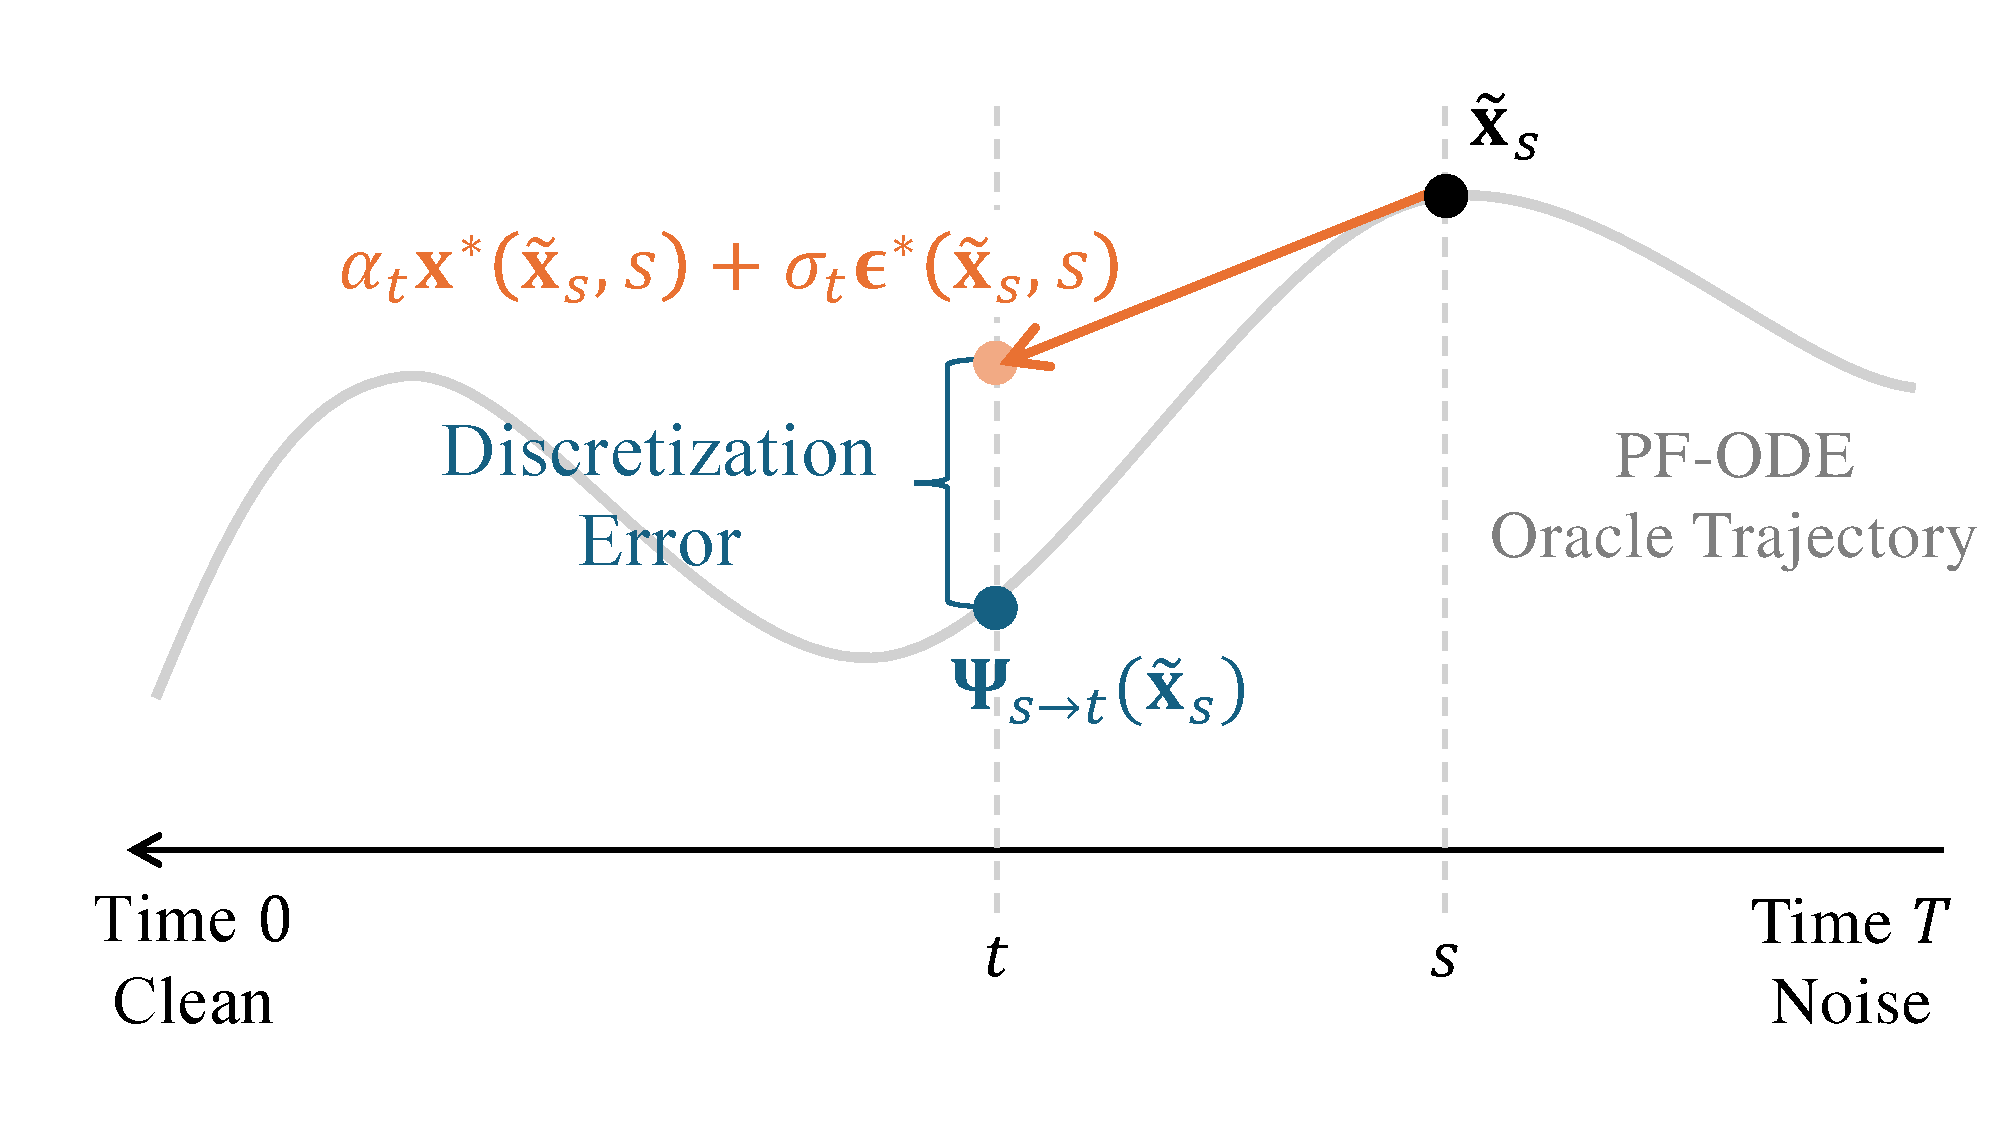
\includegraphics[width=\linewidth]{Images/PartB/Euler.pdf}
    \caption{\textbfs{将 DDIM 视为 PF-ODE 的 Euler 离散化的示意图。}  从时刻 $s$ 的状态 $\tilde\rvx_s$ 出发，真实 PF-ODE 轨迹（灰色曲线）确定性地演化到时刻 $t$ 的 $\bPsi_{s\to t}(\tilde\rvx_s)$。相比之下，DDIM 更新（橙色）直接将 $\tilde\rvx_s$ 映射到 $\alpha_t \rvx^*(\tilde\rvx_s,s) + \sigma_t \beps^*(\tilde\rvx_s,s)$。该 Euler 步与真实 PF-ODE 轨迹之间的差异引入了离散化误差，以蓝色显示。如果 $t$ 远离 $s$，差异可能变得很大，从而导致生成质量下降。
\figcredit{由作者绘制。}}
    \label{fig:euler}
\end{figure}


采用速度预测时，PF-ODE 中的线性项 $f(t)\rvx$ 被吸收到目标 $\rvv^*(\rvx(t), t)=\alpha_t'\rvx_0+\sigma_t'\beps$ 之中。由微积分基本定理，
积分 $\int_s^t \alpha_\tau'\diff\tau$ 与 $\int_s^t \sigma_\tau'\diff\tau$
简化为 $(\alpha_t-\alpha_s)$ 与 $(\sigma_t-\sigma_s)$，因此单个 Euler 步
就已经给出闭式的 DDIM 更新：
\[
\tilde\rvx_t = \alpha_t \tilde\rvx^*(\tilde\rvx_s,s) + \sigma_t \tilde\beps^*(\tilde\rvx_s,s).
\]

也就是说，采用 $\rvv$-预测时，PF-ODE 漂移中不存在需要单独分离的线性项，
因此朴素 Euler 更新自然地与 DDIM 表述一致。
相比之下，在 $\beps$-、$\rvx$-或 $\rvs$-预测参数化下，
PF-ODE 漂移可以分解为\emph{半线性}形式，由一个线性项和一个非线性修正构成，
这符合 \Cref{eq:general-semilinear-pfode} 给出的一般模板。于是，朴素的 Euler 步只能\emph{近似}线性项，而非精确计算它
（见 \Cref{eq:euler-step} 中的论证）。而 DDIM 对应于一种\emph{指数 Euler}（积分因子）步，
它解析地处理这一线性分量。
因此，$\rvv$-预测带来了最简单、最直接的 Euler 积分，
而其它参数化则需要指数 Euler 形式才能达到相同的 DDIM 行为。

上面的讨论也呼应了 \Cref{subsec:concept-why-v-affine} 中提出的论证，
并导出如下结论：
\msg{观察}{（指数）Euler 与 DDIM 更新}{
给定相同的调度器 $(\alpha_t,\sigma_t)$，
\begin{align*}
\text{$\rvv$-预测：} 
&\quad \text{Euler} = \text{DDIM}, \\[4pt]
\text{$\beps$-、$\rvx$-或 $\rvs$-预测：} 
&\quad \text{exp--Euler} = \text{DDIM} \neq \text{plain Euler},
\end{align*}
其中在 $\beps$-、$\rvx$-或 $\rvs$-预测情形下，朴素 Euler 步不等价于 DDIM，
因为线性项仅是被近似，可能导致稳定性降低。
}





\paragraph{不同参数化下 DDIM 的示例。}
我们用一个基于 \Cref{eq:ddim-update-all}、采用真实替换（$\beps^*$、$\rvx^*$、$\nabla_\rvx\log p_t$ 与 $\rvv^*$）的简单示例来说明。
假设前向核 $\alpha_t=1$ 且 $\sigma_t=t$~\citep{karras2022elucidating}。DDIM（exp--Euler）更新
\[
\tilde\rvx_{t} = \frac{\alpha_{t}}{\alpha_{s}}\tilde\rvx_{s}
- \alpha_{t} \left(\frac{\sigma_{s}}{\alpha_{s}} - \frac{\sigma_{t}}{\alpha_{t}}\right)
\beps^*(\tilde\rvx_{s}, s)
\]
简化为
\[
\tilde\rvx_t = \tilde\rvx_s - (s-t)\,\beps^*(\tilde\rvx_s,s).
\]
直观上，减去时间间隔 $(s-t)$ 与真实噪声估计
$\beps^*(\tilde\rvx_s,s)$ 的乘积，会将当前样本 $\tilde\rvx_s$ 推向更干净的估计。

使用 $\rvx$-预测的真实值 $\rvx^*$，它与噪声真实值的关系为
\[
\beps^*(\tilde\rvx_s,s) = \frac{\tilde\rvx_s - \rvx^*(\tilde\rvx_s, s)}{s},
\]
得到
\begin{align}\label{eq:ctm-formulation}
    \tilde\rvx_t
 = \tilde\rvx_s - \frac{s-t}{s}\,\bigl(\tilde\rvx_s - \rvx^*(\tilde\rvx_s, s)\bigr)
 = \frac{t}{s}\,\tilde\rvx_s + \Bigl(1-\frac{t}{s}\Bigr)\,\rvx^*(\tilde\rvx_s, s).
\end{align}
因此，$\tilde\rvx_t$ 是当前样本 $\tilde\rvx_s$ 与 $\rvx$-预测 $\rvx^*(\tilde\rvx_s, s)$（作为干净数据的真实估计）的凸组合。进一步地，我们可将其改写为
\[
\tilde\rvx_t-\rvx^* = \frac{t}{s}\,\bigl(\tilde\rvx_s-\rvx^*\bigr),\quad t<s,
\]
这表明去噪残差在每步按因子 $t/s\in(0,1)$ 收缩（因此当 $t<s$ 时不会出现超调）。

使用分数真实值，它与噪声真实值的关系为
\[
\beps^*(\tilde\rvx_s, s) = -\sigma_s \nabla_{\rvx}\log p_s(\tilde\rvx_s),
\]
DDIM（exp--Euler）更新变为
\[
\tilde\rvx_t = \tilde\rvx_s + (s-t)\,s\,\nabla_{\rvx}\log p_s(\tilde\rvx_s).
\]
这使 $\tilde\rvx_s$ 沿分数场上坡移动（朝更高似然区域），步长与时间间隔 $(s-t)$ 和噪声尺度 $s$ 成正比。

最后，使用速度真实值 $\rvv^*(\tilde\rvx_s,s) = \beps^*(\tilde\rvx_s,s)$，DDIM 更新可写为
\[
\tilde\rvx_t = \tilde\rvx_s + (t-s)\,\rvv^*(\tilde\rvx_s,s),
\]
于是割线斜率满足有限差分恒等式
\[
\frac{\tilde\rvx_t-\tilde\rvx_s}{t-s} = \rvv^*(\tilde\rvx_s,s).
\]
直观上，这意味着更新是沿局部 ODE 漂移方向的直线步。


\paragraph{DDIM 的挑战。}
作为一阶方法，DDIM 的全局离散化误差为
$\mathcal O(h)$，其中 $h:=\max_i |t_i-t_{i-1}|$。相应地，其
精度通常随步长增大而下降。这促使了高阶求解器的出现，
它们使用更丰富的局部近似把全局阶数提升到 $\mathcal O(h^k)$（$k\ge 2$）。
经过合适的时间步分配，这类方法可在更少的步数下达到目标质量。
然而，单凭更高阶并不能保证实际耗时更低，
因为每步可能需要多次模型求值。
在实践中，效率的相关度量是函数评估次数 $\mathrm{NFE}=mN$，
因此“更快”意味着以更小的 NFE 达到期望的质量，而不仅仅是更少的步数。

这个全局 $\mathcal O(h)$ 的论断虽然正确，但过于粗略，
无法解释为何某些 PF-ODE 轨迹即使在相对大的步长下也能保持良好的近似，
而另一些则不然。更具信息量的视角是询问：DDIM 在每一步冻结的是什么量，
以及该量沿精确轨迹变化有多大。

\paragraph{真正决定 DDIM 一阶误差的因素。}
一个重要的澄清是，参数化的选择\emph{并不}改变精确的真实 PF-ODE 轨迹。
在 \Cref{eq:predictions-equivalence} 的真实恒等式下，
$\rvv$-、$\beps$-、$\rvx$-与 $\rvs$-参数化只是同一 ODE 的不同表示。
所改变的只是漂移写出的形式，从而是一阶离散化把哪个量当作近似常数来处理。

\subparagraph{$\rvv$-预测情形（DDIM = Euler）。}
对 $\rvv$-预测，DDIM 恰好是对
\[
\frac{\diff \rvx(\tau)}{\diff \tau}=\rvv(\rvx(\tau),\tau).
\]
的朴素 Euler 步。
设 $h:=s-t>0$，其中 $s>t$。从时刻 $s$ 的精确状态 $\rvx_s$ 出发，
单步 DDIM/Euler 更新为
\[
\tilde{\rvx}_t^{\mathrm{Euler}}
=
\rvx_s-h\,\rvv(\rvx_s,s).
\]
带积分余项的 Taylor 定理给出
\[
\rvx(t)-\tilde{\rvx}_t^{\mathrm{Euler}}
=
\int_t^s (\tau-t)\,
\frac{\diff}{\diff \tau}\rvv(\rvx(\tau),\tau)\,\diff\tau,
\]
其中
\[
\frac{\diff}{\diff \tau}\rvv(\rvx(\tau),\tau)
=
\partial_\tau \rvv(\rvx(\tau),\tau)
+
\nabla_{\rvx}\rvv(\rvx(\tau),\tau)\,\rvv(\rvx(\tau),\tau).
\]
因此
\[
\|\rvx(t)-\tilde{\rvx}_t^{\mathrm{Euler}}\|
\le
\frac{h^2}{2}\,
\sup_{\tau\in[t,s]}
\Big\|
\partial_\tau \rvv(\rvx(\tau),\tau)
+
\nabla_{\rvx}\rvv(\rvx(\tau),\tau)\,\rvv(\rvx(\tau),\tau)
\Big\|.
\]
于是，对朴素 Euler 而言，相关的量是漂移沿精确轨迹求值的总时间导数
\[
\frac{\diff}{\diff \tau}\rvv(\rvx(\tau),\tau),
\]
等价地即轨迹的加速度，它度量了路径在该步内的弯曲程度。
特别地，若精确轨迹在 $[t,s]$ 上关于时间是仿射的，
则 Euler 在该步上是精确的。这是底层真实轨迹的特殊性质，
而非使用 $\rvv$-预测的一般结果。

\subparagraph{$\beps$-、$\rvx$-与 $\rvs$-预测情形（DDIM = Exp--Euler）。}
对 $\beps$-、$\rvx$-与 $\rvs$-预测，DDIM 是半线性 PF-ODE
\[
\frac{\diff \rvx(\tau)}{\diff \tau}
=
f(\tau)\rvx(\tau)+\rmN(\rvx(\tau),\tau).
\]
的指数 Euler 方法。
利用常数变易公式，
\[
\rvx(t)
=
\mathcal E(s\shortrightarrow t)\rvx_s
+
\int_s^t
\mathcal E(\tau\shortrightarrow t)\,
\rmN(\rvx(\tau),\tau)\,\diff\tau,
\qquad
\mathcal E(s\shortrightarrow t)
:=
\exp\!\Big(\int_s^t f(u)\,\diff u\Big),
\]
相应的指数 Euler 步为
\[
\tilde{\rvx}_t^{\mathrm{Exp}\text{-}\mathrm{Euler}}
=
\mathcal E(s\shortrightarrow t)\rvx_s
+
\left(\int_s^t \mathcal E(\tau\shortrightarrow t)\,\diff\tau\right)
\rmN(\rvx_s,s).
\]
将两个表达式相减得到精确恒等式
\[
\rvx(t)-\tilde{\rvx}_t^{\mathrm{Exp}\text{-}\mathrm{Euler}}
=
\int_s^t
\mathcal E(\tau\shortrightarrow t)\,
\Big(
\rmN(\rvx(\tau),\tau)-\rmN(\rvx_s,s)
\Big)\,\diff\tau.
\]
因此局部误差并非由 $\rvx(\tau)$ 字面意义上的笔直程度控制，
而是由非线性残差 $\rmN$ 沿精确轨迹的变化量控制。
若 $\mathcal E(\tau\shortrightarrow t)$ 在 $[t,s]$ 上有界，则
\[
\|\rvx(t)-\tilde{\rvx}_t^{\mathrm{Exp}\text{-}\mathrm{Euler}}\|
\le
\left(\sup_{\tau\in[t,s]}|\mathcal E(\tau\shortrightarrow t)|\right)
\frac{h^2}{2}\,
\sup_{\tau\in[t,s]}
\Big\|
\frac{\diff}{\diff \tau}\rmN(\rvx(\tau),\tau)
\Big\|,
\]
其中
\[
\frac{\diff}{\diff \tau}\rmN(\rvx(\tau),\tau)
=
\partial_\tau \rmN(\rvx(\tau),\tau)
+
\nabla_{\rvx}\rmN(\rvx(\tau),\tau)\,
\bigl(f(\tau)\rvx(\tau)+\rmN(\rvx(\tau),\tau)\bigr).
\]
特别地，每当 $\rmN(\rvx(\tau),\tau)$ 在该区间上保持常数时，
指数 Euler 在该步上是精确的。

要点并不在于某种参数化使真实 PF-ODE 轨迹变得“笔直”。
相反，少步精度由所选一阶格式所冻结的量沿精确轨迹变化的大小控制：
对朴素 Euler 是漂移 $\rvv$，对指数 Euler 是非线性残差 $\rmN$。
这也澄清了为何一般性的全局 $\mathcal O(h)$ 论断在实践中可能过于粗略。
两条轨迹可能具有截然不同的少步行为，
即使这种最坏情形的界看起来相似，
因为实际的单步误差由所实现的真实路径上的相应导数决定。

上文的讨论仅涉及数值求解器的离散化误差；在实践中，
总采样误差还包括模型失配以及所学网络中的近似误差。


\subsection{（可选）DDIM 的变分视角}\label{subsec:ddim}

事实上，DDIM 的动机来自通过变分视角重新审视 DDPM。
在 DDPM 中，反向过程与一个特定的马尔可夫前向转移核
$p(\rvx_t|\rvx_{t-\Delta t})$ 绑定，它强制要求小的步长
以便正确地近似多步后验。DDIM 摆脱了这一限制，
它观察到训练目标仅依赖于边缘扰动 $p_t(\rvx_t|\rvx_0)$，
而不依赖于具体的前向转移。这一洞察使我们能够直接从边缘构造反向动力学，
因此可以在保持边缘一致性的同时跳过中间步骤。
由于该转移被定义为对任意 $t<s$ 都将 $p_s(\rvx_s|\rvx_0)$ 映射到
$p_t(\rvx_t|\rvx_0)$，我们可以使用一个粗的时间网格，
其更新次数要少得多，从而减少模型求值次数，实现快速的少步采样。



\paragraph{重新审视 DDPM 的变分视角。}
在 DDPM 中，训练固定了一族边缘扰动核
$p_t(\rvx_t|\rvx_0)$ 并优化一个仅依赖于这些边缘的代理目标。
然而在采样时，反向条件分布是单步前向核下的贝叶斯后验：
\[
p(\rvx_{t-\Delta t}|\rvx_t,\rvx_0)
= \frac{p(\rvx_t|\rvx_{t-\Delta t})\,p_{t-\Delta t}(\rvx_{t-\Delta t}|\rvx_0)}
       {p_t(\rvx_t|\rvx_0)}.
\]
这把反向更新与\emph{特定}的前向转移 $p(\rvx_t|\rvx_{t-\Delta t})$ 绑定在一起。
如果人们试图通过增大 $\Delta t$ 同时复用相同的单步核来跳过步骤，
那么这就不再匹配真实的多步后验，通常会损害边缘分布。


\paragraph{DDIM 的原始动机。}
DDIM 观察到训练目标仅约束边缘 $p_t(\rvx_t|\rvx_0)$，而不约束
中间的反向转移。因此，人们可以\emph{指定}一族反向条件分布
${\color{orange}\pi(\rvx_t|\rvx_s,\rvx_0)}$（对任意 $t<s$），使其满足\emph{单步边缘一致性}\footnote{如果我们把 \Cref{eq:ddim-reverse-kernel-def} 中的“用户定义”反向转移核
$\pi$ 选为与“真实”条件分布完全相同：
${\color{orange}\pi(\rvx_t|\rvx_s,\rvx_0)} = p(\rvx_t|\rvx_s, \rvx_0)$，
则边缘一致性条件
   \[
\int {\color{orange}\pi(\rvx_t|\rvx_s,\rvx_0)}\,p_s(\rvx_s|\rvx_0)\diff \rvx_s
= p_t(\rvx_t|\rvx_0)
\] 
仅仅是条件联合分布的\emph{全概率法则}（也称\emph{塔性质}）的推论：
\[
p_t(\rvx_t|\rvx_0)
= \int p(\rvx_t,\rvx_s|\rvx_0)\diff \rvx_s
= \int p(\rvx_t|\rvx_s,\rvx_0)\,p_s(\rvx_s|\rvx_0)\diff \rvx_s.
\]
或者等价地，将贝叶斯后验显式地写成
\[
p(\rvx_t|\rvx_s,\rvx_0)
= \frac{p(\rvx_s|\rvx_t,\rvx_0)\,p_t(\rvx_t|\rvx_0)}
       {p_s(\rvx_s|\rvx_0)},
\]
然后两端乘以 $p_s(\rvx_s|\rvx_0)$ 并对 $\rvx_s$ 求边缘，我们恢复
\[
\int p(\rvx_t|\rvx_s,\rvx_0)\,p_s(\rvx_s|\rvx_0) \diff \rvx_s
= p_t(\rvx_t|\rvx_0),
\]
这恰好是相同的边缘一致性条件。

在马尔可夫前向情形下，进一步有
$p(\rvx_t|\rvx_s,\rvx_0)=p(\rvx_t|\rvx_s)$，
从而下式化简为：
\[
p_t(\rvx_t|\rvx_0)
= \int p(\rvx_t|\rvx_s)\,p_s(\rvx_s|\rvx_0)\diff \rvx_s.
\]
}：
\begin{mdframed}
    \begin{align}\label{eq:ddim-reverse-kernel-def}
\int {\color{orange}\pi(\rvx_t|\rvx_s,\rvx_0)}\,p_s(\rvx_s|\rvx_0) \diff \rvx_s
= p_t(\rvx_t|\rvx_0).
\end{align}
\end{mdframed}
这种构造消除了对前向单步核 $p(\rvx_t|\rvx_{t-\Delta t})$ 的任何依赖，
并为粗（跳过的）时间步提供了合法性。

\paragraph{离散时间 DDIM 的推导。}
考虑一般的前向扰动：
\begin{equation*}
    p_t(\rvx_t|\rvx_0) := \mathcal{N}\big(\rvx_t; \alpha_t \rvx_0, \sigma_t^2 \mathbf{I}\big),
\end{equation*}
其中 $\rvx_0 \sim p_{\mathrm{data}}$。


DDIM 不要求反向更新与绑定到
单步前向核的贝叶斯后验一致。只需\emph{选择}一个保持
边缘的反向条件分布即可。具体地，对任意 $t<s$ 我们假定高斯族
\begin{align}\label{eq:ddim-reverse-kernel-param}
{\color{orange}\pi(\rvx_t|\rvx_s,\rvx_0)}
= \mathcal{N} \big(\rvx_t;\, a_{t,s}\,\rvx_0 + b_{t,s}\,\rvx_s,\; c_{t,s}^2\,\mathbf{I}\big),
\end{align}
其系数 $(a_{t,s},b_{t,s},c_{t,s})$ 由边缘一致性
约束 \Cref{eq:ddim-reverse-kernel-def} 确定。由于所有涉及的核都是高斯的，
按 \Cref{eq:ddim-reverse-kernel-param} 从 $\rvx_s|\rvx_0=\alpha_s\rvx_0+\sigma_s\beps'$ 采样，然后再采样
$\rvx_t|\rvx_s,\rvx_0$，得到
\begin{align}\label{eq:ddim-derivation} 
\begin{aligned}
\rvx_t
&= a_{t,s}\,\rvx_0 + b_{t,s}\,\rvx_s + c_{t,s}\,\beps
\\&= a_{t,s}\,\rvx_0 + b_{t,s}\big(\alpha_s\rvx_0+\sigma_s\beps'\big) + c_{t,s}\,\beps \\
&= (a_{t,s} + b_{t,s}\alpha_s)\,\rvx_0
+ \sqrt{b_{t,s}^2\sigma_s^2 + c_{t,s}^2}\;\beps'',
\end{aligned}
\end{align}
其中 $\beps,\beps',\beps''\sim\mathcal{N}(\mathbf{0},\mathbf{I})$ 相互独立（高斯可加性）。
另一方面，
\[
\rvx_t\sim p_t(\rvx_t|\rvx_0)
= \mathcal{N} \big(\rvx_t; \alpha_t\rvx_0, \sigma_t^2\mathbf{I}\big).
\]
令此目标与 \Cref{eq:ddim-derivation} 的均值和方差相等，得到
\begin{align*}
\alpha_t = a_{t,s} + b_{t,s}\alpha_s,
\qquad
\sigma_t^2 = b_{t,s}^2\sigma_s^2 + c_{t,s}^2.
\end{align*}
这个方程组是欠定的，因此我们把 $c_{t,s}$ 视为带有自然约束
$0\le c_{t,s} \le \sigma_t$ 的自由参数，求解 $a_{t,s},b_{t,s}$：
\begin{align}\label{eq:ddim-coefficients}
b_{t,s} = \frac{\sqrt{\sigma_t^2 - c_{t,s}^2}}{\sigma_s},
\qquad
a_{t,s} = \alpha_t - \alpha_s\,b_{t,s}.
\end{align}
这里我们不失一般性地取 $b_{t,s}$ 的非负根。

将 \Cref{eq:ddim-coefficients} 代入 \Cref{eq:ddim-reverse-kernel-param} 得到
\begin{align}\label{eq:ddim-reverse-kernel-result}
{\color{orange}\pi(\rvx_t|\rvx_s,\rvx_0)}
= \mathcal{N} \Big(
\rvx_t;\;
\underbrace{\alpha_t\rvx_0
+ \frac{\sqrt{\sigma_t^2 - c_{t,s}^2}}{\sigma_s}\,(\rvx_s - \alpha_s\rvx_0)}_{\text{mean}},
\;\; c_{t,s}^2\mathbf{I}\Big).
\end{align}
等价地，\Cref{eq:ddim-reverse-kernel-result} 中的均值展开为
\[
\Big(\alpha_t - \alpha_s\frac{\sqrt{\sigma_t^2 - c_{t,s}^2}}{\sigma_s}\Big)\rvx_0
+ \Big(\frac{\sqrt{\sigma_t^2 - c_{t,s}^2}}{\sigma_s}\Big)\rvx_s.
\]

\lem{DDIM 系数}{ddim-coeff}{
设 ${\color{orange}\pi(\rvx_t|\rvx_s,\rvx_0)}$ 由 \Cref{eq:ddim-reverse-kernel-param} 给出。
若边缘一致性条件 \Cref{eq:ddim-reverse-kernel-def} 成立，则系数
恰好是 \Cref{eq:ddim-coefficients} 中的那些，其中 $0\le c_{t,s}\le \sigma_t$。
}

\rmkb{
\begin{enumerate}[leftmargin=*]
    \item 在 DDIM 中，我们\emph{选择}反向核 ${\color{orange}\pi(\rvx_t|\rvx_s,\rvx_0)}$ 满足
边缘一致性约束，而一般地
\[
{\color{orange}\pi(\rvx_t|\rvx_s,\rvx_0)}\neq p (\rvx_t|\rvx_s,\rvx_0),
\]
其中 $p (\rvx_t|\rvx_s,\rvx_0)$ 是与特定前向
单步核相关联的贝叶斯后验。由贝叶斯法则，
\[
p(\rvx_t|\rvx_s,\rvx_0)\;\propto\; p(\rvx_s|\rvx_t)\,p_t(\rvx_t|\rvx_0),
\]
此后验\emph{并不}是规定 $\pi$ 或训练所必需的。
    \item 仅在选择方差参数以匹配 DDPM 后验
方差的特殊情形下（即 \Cref{eq:eta-ddim} 中 $\eta=1$ 的设定），才有 ${\color{orange}\pi(\rvx_t|\rvx_s,\rvx_0)}=
p (\rvx_t|\rvx_s,\rvx_0)$；否则 ${\color{orange}\pi(\rvx_t|\rvx_s,\rvx_0)} \neq
p (\rvx_t|\rvx_s,\rvx_0)$。
    \item 不施加马尔可夫约束时，一般地 $p(\rvx_s|\rvx_t,\rvx_0)\neq p(\rvx_s|\rvx_t)$。
等式 $p(\rvx_s|\rvx_t,\rvx_0)=p(\rvx_s|\rvx_t)$ 绑定于一个特定的马尔可夫前向模型，
而 DDIM 在其反向构造中并不假设该模型。
\end{enumerate}
}


前向边缘 $\{p_t(\rvx_t|\rvx_0)\}_t$ 并不唯一地确定反向条件
转移。存在无穷多个满足
\Cref{eq:ddim-reverse-kernel-def} 的核
${\color{orange}\pi(\rvx_t|\rvx_s,\rvx_0)}$，其中任何一个都可以自由地规定。
参数 $c_{t,s}$ 为这一族建立索引，并控制
每次反向步 $s \to t$ 注入的噪声量。下面，我们介绍这一族 DDIM 求解器。





\paragraph{DDIM 采样器（步 $s\to t$）。}
DDIM 采样器由所选反向核 \Cref{eq:ddim-reverse-kernel-result} 中的 ${\color{orange}\pi(\rvx_t|\rvx_s,\rvx_0)}$，
通过用预训练模型的预测器替换 $\rvx_0$ 而得到。
使用 $\beps$-预测网络 $\beps_{\bm{\phi}^\times}$（即插即用，无需重训），令
\[
\rvx_{\bm{\phi}^\times}(\rvx_s,s)
:= \frac{\rvx_s - \sigma_s\,\beps_{\bm{\phi}^\times}(\rvx_s,s)}{\alpha_s},
\quad
p_{\bm{\phi}^\times}(\rvx_t|\rvx_s)
:= {\color{orange}\pi\big(\rvx_t\,\big|\,\rvx_s,\rvx_{\bm{\phi}^\times}(\rvx_s,s)\big)}.
\]
将 $\rvx_{\bm{\phi}^\times}$ 代入 \Cref{eq:ddim-reverse-kernel-result} 得到更新
\begin{mdframed}
\[
\rvx_t
= \frac{\alpha_t}{\alpha_s}\,\rvx_s
+\Big(\sqrt{\sigma_t^2 - c_{t,s}^2}-\frac{\alpha_t}{\alpha_s}\sigma_s\Big)\,
\beps_{\bm{\phi}^\times}(\rvx_s,s)
+ c_{t,s}\,\beps_t,
\quad \beps_t\sim\mathcal{N}(\mathbf{0},\mathbf{I}),
\]
\end{mdframed}
其中 $c_{t,s}\in[0,\sigma_t]$ 控制随机性。

为记号方便，定义前向因子
\[
\alpha_{t|s}:=\tfrac{\alpha_t}{\alpha_s},
\qquad
\sigma_{t|s}^2:=\sigma_t^2-\alpha_{t|s}^2\,\sigma_s^2,
\]
使得 $p(\rvx_t|\rvx_s)=\mathcal{N}(\alpha_{t|s}\rvx_s,\sigma_{t|s}^2\mathbf{I})$。于是采样器可写为
\[
\rvx_t
= \alpha_{t|s}\,\rvx_s
+\big(\sqrt{\sigma_t^2 - c_{t,s}^2}-\alpha_{t|s}\sigma_s\big)\,
\beps_{\bm{\phi}^\times}(\rvx_s,s)
+ c_{t,s}\,\beps_t.
\]

通过改变 $c_{t,s}$，可得到一族共享同一预训练扩散模型且无需重训的采样器：
\begin{itemize}
\item \textbfs{DDPM 步（后验方差）：}
$
c_{t,s}=\frac{\sigma_s}{\sigma_t}\,\sigma_{t|s}
$
使 ${\color{orange}\pi(\rvx_t|\rvx_s,\rvx_0)}$ 等于由单步前向核诱导的贝叶斯后验
$p(\rvx_t|\rvx_s,\rvx_0)$。
用其预测器替换 $\rvx_0$ 得到标准 DDPM 反向更新
$p_{\bm{\phi}^\times}(\rvx_t|\rvx_s)$，即在 $\alpha_t^2+\sigma_t^2=1$ 下的马尔可夫 DDPM 步（\Cref{eq:ddpm-sampling}）。

\item \textbfs{确定性 DDIM（$\eta=0$）：}
$
c_{t,s}=0
$
给出
\[
\rvx_t
= \alpha_{t|s}\rvx_s + \big(\sigma_t-\alpha_{t|s}\sigma_s\big)\beps_{\bm{\phi}^\times}(\rvx_s,s),
\]
与 ODE 视角下的 DDIM 跳跃一致。

\item \textbfs{插值：} 定义
\begin{align}\label{eq:eta-ddim}
    c_{t,s}=\eta\,\frac{\sigma_s}{\sigma_t}\,\sigma_{t|s}, \quad \eta\in[0,1],
\end{align}
使得 $\eta$ 在随机 DDPM 更新（$\eta=1$）与确定性 DDIM 更新（$\eta=0$）之间平滑插值。
\end{itemize}





\subsection{作为条件流匹配的 DDIM}\label{subsec:ddim-cfm}
本小节将看到，确定性 DDIM 可以被理解为寻找一个条件流映射，它把 $p_s(\cdot|\rvx_0)$ 前推到 $p_t(\cdot|\rvx_0)$。
此条件流的切线与条件流匹配（CFM）中使用的条件速度一致。
对该条件速度取边缘便得到 PF--ODE 漂移，其朴素 Euler 离散化恢复了 $\rvv$-预测下的边缘 DDIM 更新。

我们重新审视 DDIM 单步条件边缘一致性恒等式（\Cref{eq:ddim-reverse-kernel-def}）
\[
\int {\color{orange}\pi(\rvx_t|\rvx_s,\rvx_0)} p_s(\rvx_s|\rvx_0) \diff \rvx_s
= p_t(\rvx_t|\rvx_0), \quad t<s,
\]
即若 $\rvx_s\sim p_s(\cdot|\rvx_0)$，则用所选反向核前推 $\rvx_s$ 可复现 $p_t(\cdot|\rvx_0)$。
当反向核为确定性时，它等价于寻找一个条件映射
$\bPsi_{s\to t}(\cdot|\rvx_0)$，把 $p_s(\cdot|\rvx_0)$ 前推到 $p_t(\cdot|\rvx_0)$：
\[
{\color{orange}\pi(\rvx_t|\rvx_s,\rvx_0)}
=\delta \big(\rvx_t-\bPsi_{s\to t}(\rvx_s|\rvx_0)\big),
\qquad
\bigl(\bPsi_{s\to t}(\cdot|\rvx_0)\bigr)_{\#}p_s(\cdot|\rvx_0)=p_t(\cdot|\rvx_0).
\]


在线性--高斯路径 $\rvx_\tau=\alpha_\tau\rvx_0+\sigma_\tau\beps$ 下，
类似于 \Cref{eq:ddim-reverse-kernel-param,eq:ddim-derivation} 的论证
给出\textit{条件映射}
\[
\bPsi_{s\to t}(\rvx_s|\rvx_0)
=\frac{\sigma_t}{\sigma_s}\,\rvx_s
+\Bigl(\alpha_t-\alpha_s\frac{\sigma_t}{\sigma_s}\Bigr)\rvx_0,
\]
其瞬时的\textit{条件速度}为
\[
\rvv_t^{*}(\rvx|\rvx_0)
=\partial_h \big|_{h=0}\bPsi_{t\to t+h}(\rvx|\rvx_0)
=\frac{\sigma_t'}{\sigma_t}\,\rvx
+\Bigl(\alpha_t'-\alpha_t\frac{\sigma_t'}{\sigma_t}\Bigr)\rvx_0.
\]
我们将 $\bPsi_{s\to t}(\cdot|\rvx_0)$ 称为 DDIM 条件映射。

有了 $p_t(\rvx|\rvx_0)$，条件流匹配把时间依赖场拟合到此目标速度，
\[
\mathcal L_{\mathrm{CFM}}(\bphi)
=\E_{t,\rvx_0,\rvx_t\sim p_t(\cdot|\rvx_0)}
\big\|\rvv_\bphi(\rvx_t,t)-\rvv_t^{*}(\rvx_t|\rvx_0)\big\|^2,
\]
因此 CFM 的回归目标等于 DDIM 条件映射的条件速度。

\msg{观察}{条件层面}{
沿条件高斯路径，DDIM 条件映射与 CFM 目标生成相同的条件流 $\bPsi_{s\to t}(\cdot|\rvx_0)$。
}

在给定 $\rvx_t=\rvx$ 下对 $\rvx_0$ 的后验求条件速度的平均，得到边缘 PF--ODE 漂移，
\[
\rvv^*(\rvx,t)=\E \left[\rvv_t^*(\rvx| \rvx_0)|\rvx_t=\rvx\right],
\]
它在线性--高斯调度下取可分离的预测器形式
\[
\rvv^*(\rvx,t)=\alpha_t'\,\rvx^*(\rvx,t)+\sigma_t'\,\beps^*(\rvx,t),
\quad
\rvx=\alpha_t\,\rvx^*(\rvx,t)+\sigma_t\,\beps^*(\rvx,t).
\]
我们已经看到，对此取过边缘的 $\rvv$-预测的 PF-ODE，其朴素 Euler 步恰好是 DDIM 更新（\Cref{eq:ddim-update-all} 中最后的恒等式）。

简言之，DDIM 是（i）一个确定性条件传输，其切线等于 CFM 目标；（ii）对该切线取边缘后，是 PF--ODE 的一个 Euler 步，其步恰好与 DDIM 更新一致。


\newpage


% \paragraph{(Optional, move to appendix) Gauge freedom and rotations}
% More generally, one may replace the shared-noise coupling with any orthogonal transformation
% $\rmR_{s\to t}\in\mathrm{O}(D)$, yielding
% \[
% \rmT^{\rvx_0}_{s\to t}(\rvx_s)
% =\frac{\sigma_t}{\sigma_s}\,\rmR_{s\to t}\,\rvx_s
% +\Big(\alpha_t-\alpha_s\frac{\sigma_t}{\sigma_s}\,\rmR_{s\to t}\Big)\rvx_0,
% \qquad
% \beps_t=\rmR_{s\to t}\beps_s.
% \]
% Each such choice preserves the marginal consistency condition, introducing a \emph{gauge freedom} in the noise rotation.
% For the maps to compose consistently across time, the rotations must satisfy the cocycle (semigroup) rule
% \[
% \rmR_{s\to t}=\rmR_{u\to t}\,\rmR_{s\to u},\qquad
% \rmR_{t\to t}=\rmI.
% \]
% DDIM corresponds to the simplest gauge, $\rmR_{s\to t}=\rmI$, where all noise directions are aligned (shared across time).
% Since this specific gauge already yields the standard DDIM flow and serves as the target for CFM,
% the broader rotation family is optional and mainly of theoretical interest.

%%%%%%%%%%%%%%%%%%%%%%%%%%%%
% In this subsection, we further focus on the discussion on the (variational perspective) DDIM marginal-consistency identity (\Cref{eq:ddim-reverse-kernel-def})
% \begin{align*}
% \int {\color{orange}\pi(\rvx_t|\rvx_s,\rvx_0)}p_s(\rvx_s|\rvx_0)\diff \rvx_s
% = p_t(\rvx_t|\rvx_0), \quad t<s.
% \end{align*}
% It states that, if $\rvx_s\sim p_s(\cdot|\rvx_0)$, then pushing $\rvx_s$ forward by the
% user-specified kernel ${\color{orange}\pi(\cdot|\rvx_s,\rvx_0)}$ produces the correct later marginal
% $p_t(\cdot|\rvx_0)$.


% \paragraph{Deterministic Kernels $\Rightarrow$ Pushforward Maps.}
% When the reverse kernel ${\color{orange}\pi(\rvx_t|\rvx_s,\rvx_0)}$ is chosen to be \emph{deterministic}, it can be written as a Dirac measure
% concentrated at the output of a conditional map $\rmT^{\rvx_0}_{s\to t}$:
% \[
% {\color{orange}\pi(\rvx_t|\rvx_s,\rvx_0)}
% = \delta \big(\rvx_t-\rmT^{\rvx_0}_{s\to t}(\rvx_s)\big),
% \]
% Here, $\rmT^{\rvx_0}_{s\to t}(\cdot):\R^D \to \R^D$ is a function that evolves the state from time $s$ to time $t$ given a endpoint $\rvx_0$.

% In this case, one-step marginal consistency becomes searching a conditional (on $\rvx_0$) deterministic map $\rmT^{\rvx_0}_{s\to t}$ that satisfies the  pushforward relation
% \[
% (\rmT^{\rvx_0}_{s\to t})_{\#}\,p_s(\cdot|\rvx_0)=p_t(\cdot|\rvx_0).
% \]

% \paragraph{Gaussian Forward and the General Form of a Marginal-Correct Map.}
% Assume the standard linear–Gaussian forward conditionals
% \[
% p_\tau(\rvx_\tau|\rvx_0)=\mathcal N \big(\rvx_\tau;\alpha_\tau \rvx_0,\;\sigma_\tau^2 \rmI\big),\qquad \sigma_\tau>0.
% \]
% If a deterministic map pushes $p_s(\cdot|\rvx_0)$ to $p_t(\cdot|\rvx_0)$ for \emph{all} $\rvx_0$, then (classically) it must be
% \emph{affine}:
% \[
% \rmT^{\rvx_0}_{s\to t}(\rvx_s)=\rmA_{s\to t}\rvx_0 + \rmB_{s\to t}\rvx_s,
% \]
% and matching the Gaussian mean and covariance forces
% \[
% \rmA_{s\to t}=\alpha_t\rmI-\alpha_s\frac{\sigma_t}{\sigma_s}\rmR_{s\to t},\quad 
% \rmB_{s\to t}=\frac{\sigma_t}{\sigma_s}\rmR_{s\to t}
% \]
% where $\rmR_{s\to t}$ is any $D\times D$ orthogonal matrix.
% Hence the more general deterministic, marginal-correct update (oracle case) is
% \[
% \rmT^{\rvx_0}_{s\to t}(\rvx_s)
% =\frac{\sigma_t}{\sigma_s}\rmR_{s\to t}\,\rvx_s
% +\Big(\alpha_t-\alpha_s\frac{\sigma_t}{\sigma_s}\rmR_{s\to t}\Big)\rvx_0.
% \]
% The orthogonal factor $\rmR_{s\to t}$ is a genuine \emph{gauge freedom}: it does not change the one-step marginals.


% \paragraph{Route to Standard DDIM.}
% For any fixed $\rvx_0$, if the family $\{\rmT^{\rvx_0}_{s\to t}(\cdot)\}_{s,t}$ is continuous in $t$,
% locally Lipschitz in $\rvx$, and satisfies $\rmT^{\rvx_0}_{t\to t}=\mathrm{Id}$, then it constitutes the
% \emph{conditional flow map} (evolution family) of an ODE. We write this conditional flow map as $ \bPsi_{s\to t}(\cdot|\rvx_0)$ to replace $\rmT^{\rvx_0}_{s\to t}(\cdot)$. Its conditional velocity is derived (?) defined (?) in the following sense: by taking time differentiation:
% \[
% \rvv_t(\rvx|\rvx_0):= \lim_{h\to 0}\frac{\big(\bPsi_{t\to t+h}(\rvx|\rvx_0)-\rvx\big)}{h}, \quad\text{for any }\, t
% \]
% whenever the limit exists. Standard existence and uniqueness results for ODEs then ensure that this conditional
% vector field generates the given  conditional flow (i.e., the  continuity equation is fulfilled). 

% Since $ \bPsi_{s\to t}(\cdot|\rvx_0)$ is an ODE flow map, the following holds automatically by uniqueness, which is known as \emph{semigroup property} for flow maps:
% \[
% \bPsi_{s\to t}(\cdot|\rvx_0)=\bPsi_{u\to t}(\cdot|\rvx_0) \circ \bPsi_{s\to u}(\cdot|\rvx_0),
% \quad
% \bPsi_{t\to t}(\cdot|\rvx_0)=\mathrm{Id}.
% \]
% This implies the rotation matrix (gauge freedom) $\rmR_{s\to t}$ needs to satisfies: 
% \[
% \rmR_{s\to t} = \rmR_{u\to t} \circ \rmR_{s\to u},
% \]
% while there are infinitely many choices for this rotation matrix.

% In the standard DDIM, condition on $\rvx_0$ and pick the path $\rvx_t=\alpha_t \rvx_0+\sigma_t\beps$ with \emph{shared} $\beps$. It fixes the gauge freedom by the \emph{shared-noise}  $\beps\sim \mathcal{N}(\bm{0}, \rmI)$ choice:
% \[
% \beps_t=\beps_s=\beps,\quad \text{for any }\, s>t.
% \]
% This is equivalent to enforcing   $\rmR_{s\to t}=\rmI$ for all $s>t$. 

% With this shared noise, it leads to the standard DDIM deterministic update:
% \[
% \bPsi_{s\to t}(\rvx_s| \rvx_0)
% =\frac{\sigma_t}{\sigma_s}\,\rvx_s+\Big(\alpha_t-\alpha_s\frac{\sigma_t}{\sigma_s}\Big)\rvx_0.
% \]


% \paragraph{How this Connects to Flow Matching.}

% Its time derivative gives a \emph{conditional velocity}
% \[
% \rvv_t(\rvx| \rvx_0)=\alpha_t' \rvx_0+\frac{\sigma_t'}{\sigma_t}\big(\rvx-\alpha_t\rvx_0\big).
% \]
% \emph{Conditional Flow Matching} trains a model to match this drift; integrating it recovers the DDIM map above.
% Unconditioning (averaging over $\rvx_0$ given $\rvx_t$) yields the familiar probability-flow ODE drift used in score-based samplers.

% \paragraph{Practical note.}
% At sampling time, $\rvx_0$ is unknown and replaced by a denoiser  $\rvx_{\bphi^\times}(\rvx_s,s)$, so both one-step marginal matching and semigroup hold only \emph{approximately}. Enforcing composition (CK/semigroup) during design or training can improve robustness to step size, but the core DDIM update follows already from one-step marginals plus the shared-noise gauge.


%%%%%%%%%%%%%%%%%%%%%%%%%%%%%
% \paragraph{(Optional) Chapman--Kolmogorov Identity vs.\ Semigroup Property.}
% Important: the pushforward relationship does not force different time pairs to be compatible. You can satisfy all pairs $(s,t)$ and still have
% $\rmT^{\rvx_0}_{t\to u} \circ \rmT^{\rvx_0}_{s\to t}\neq \rmT^{\rvx_0}_{s\to u}$.


% The Chapman--Kolmogorov (CK) identity composes kernels across an intermediate time:
% \[
% \pi_{s\to u}(\rvx_u|\rvx_s,\rvx_0)
% =\int \pi_{t\to u}(\rvx_u|\rvx_t,\rvx_0)\,\pi_{s\to t}(\rvx_t|\rvx_s,\rvx_0)\diff\rvx_t\quad(s>t>u).
% \]
% In the deterministic case this reduces to the \emph{semigroup property} for maps
% \[
% \rmT^{\rvx_0}_{s\to u}=\rmT^{\rvx_0}_{t\to u}\circ \rmT^{\rvx_0}_{s\to t},
% \qquad
% \rmT^{\rvx_0}_{t\to t}=\mathrm{Id}.
% \]
% CK/semigroup is strictly \emph{stronger} than one-step marginal consistency.



%%%%%%%%%%%%%%%%%%%%%%%%%%

% ---------
% DDIM relaxes the Markovian assumption in the reverse (inference) process to enable fast sampling; defining the reverse transitions as Markovian is unnecessary. Instead, infinitely many choices exist for
% $p(\rvx_{t-\Delta t}|\rvx_t, \rvx_0)$ (i.e., there are infinitely many valid reverse transition distributions that map from $\mathbf{x}_t$ to $\mathbf{x}_{t-\Delta t}$ given $\mathbf{x}_0$), as long as the marginal consistency condition is satisfied:
% \begin{align}\label{eq:marginal_ddim}
%     \int p(\rvx_{t-\Delta t}|\rvx_t, \rvx_0)   p_t(\rvx_t|\rvx_0)   \diff\rvx_t = p_{t-\Delta t}(\rvx_{t-\Delta t}|\rvx_0).
% \end{align}

% We assume that $p(\rvx_{t-\Delta t}|\rvx_t, \rvx_0)$ is Gaussian, which is natural given the Gaussian forward kernels, and take it in the form:
% \begin{align}\label{eq:ddim-reverse-kernel-def}
%     p(\rvx_{t-\Delta t}|\rvx_t, \rvx_0) := \mathcal{N}\big(\rvx_{t-\Delta t}; a_t \rvx_0 + b_t \rvx_t, c_t^2 \mathbf{I}\big),
% \end{align}
% where coefficients $a_t, b_t, c_t$ are to be determined by \Cref{eq:marginal_ddim}. Since all involved kernels are Gaussian, the marginal consistency condition expands to
% \begin{align}\label{eq:ddim-derivation}
% \begin{aligned}
%     \rvx_{t-\Delta t} 
%     &= a_t \rvx_0 + b_t \rvx_t + c_t \bm{\epsilon} \\
%     &= a_t \rvx_0 + b_t (\alpha_t \rvx_0 + \sigma_t \bm{\epsilon}') + c_t \bm{\epsilon} \\
%     &= (a_t + b_t \alpha_t) \rvx_0 + \sqrt{(b_t \sigma_t)^2 + c_t^2} \bm{\epsilon}'',
% \end{aligned}
% \end{align}
% where $\bm{\epsilon}, \bm{\epsilon}', \bm{\epsilon}'' \sim \mathcal{N}(\bm{0}, \mathbf{I})$ are independent and we used the Gaussian sum property.

% On the other hand, from the forward process,
% \[
% \rvx_{t-\Delta t} \sim p_{t-\Delta t}(\rvx_{t-\Delta t}|\rvx_0) = \mathcal{N}\big(\rvx_{t-\Delta t}; \alpha_{t-\Delta t} \rvx_0, \sigma_{t-\Delta t}^2 \mathbf{I}\big),
% \]
% so equating means and variances in \Cref{eq:ddim-derivation} yields
% \begin{align}
% \begin{cases}
%     \alpha_{t-\Delta t} = a_t + b_t \alpha_t, \\
%     \sigma_{t-\Delta t} = \sqrt{(b_t \sigma_t)^2 + c_t^2}.
% \end{cases}
% \end{align}
% Since this system is underdetermined (i.e., has infinitely many solutions), we can treat $c_t$ as a free parameter and solve for $a_t$ and $b_t$, summarizing the result in the following lemma.
% \lem{DDIM Coefficients}{ddim-coeff}{
% Define the reverse conditional kernel as in \Cref{eq:ddim-reverse-kernel-def} with coefficients $a_t, b_t, c_t$. If it satisfies the marginal condition \Cref{eq:marginal_ddim}, then
% \begin{align*}
%     a_t &= \alpha_{t-\Delta t} - \alpha_t \frac{\sqrt{\sigma_{t-\Delta t}^2 - c_t^2}}{\sigma_t}, \quad
%     b_t = \frac{\sqrt{\sigma_{t-\Delta t}^2 - c_t^2}}{\sigma_t}.
% \end{align*}
% }
% Hence,
% \begin{align}\label{eq:ddim-reverse-kernel-result}
% \begin{aligned}
%     p(\rvx_{t-\Delta t}|\rvx_t, \rvx_0) = \mathcal{N}\Bigg(&
%         \rvx_{t-\Delta t}; 
%         \left(\alpha_{t-\Delta t} - \alpha_t \frac{\sqrt{\sigma_{t-\Delta t}^2 - c_t^2}}{\sigma_t}\right) \rvx_0 \\
%         &\quad+ \left(\frac{\sqrt{\sigma_{t-\Delta t}^2 - c_t^2}}{\sigma_t}\right) \rvx_t,
%         c_t^2 \mathbf{I}
%     \Bigg).
% \end{aligned}
% \end{align}
% \rmkb{
% Note that in the DDIM setup, in general,
% \[
% p(\rvx_t|\rvx_{t-\Delta t}, \rvx_0) \neq p(\rvx_t|\rvx_{t-\Delta t}),
% \]
% since the Markov assumption is not imposed. An analogous identity from Bayes' rule states that
% \[
% p(\rvx_{t-\Delta t}|\rvx_t, \rvx_0) = p(\rvx_t|\rvx_{t-\Delta t}, \rvx_0) \frac{p_{t-\Delta t}(\rvx_{t-\Delta t}|\rvx_0)}{p_t(\rvx_t|\rvx_0)}.
% \]
% Although we can compute $p(\rvx_t|\rvx_{t-\Delta t}, \rvx_0)$ using this identity, it is generally not used for training or sampling.\dk{Isn't it used to derive Eq. (2.2.3)? Other than thsi Bayes rule, how could we derive the loss function?}
% }
% Until now, we emphasize the key insight behind the DDIM approach from a variational perspective:
% \msg{Insight}{}{
% The forward marginal distributions $\{p_t(\rvx_t|\rvx_0)\}_t$ alone do not uniquely determine the reverse conditional transitions; in fact, there are infinitely many $p(\rvx_{t-\Delta t}|\rvx_t, \rvx_0)$ satisfying the marginal consistency (e.g., parameterized by $c_t$).
% }



% \paragraph{Discrete-Time DDIM Sampler.}  
% The key difference between DDIM and the formulation in DDPM (\Cref{sec:variational-perspective}) lies in modeling the conditional distribution $p(\rvx_{t-\Delta t}|\rvx_t, \rvx_0)$. Thus, DDIM enables a plug-and-play approach\footnote{See Theorem 1 in \citep{song2020denoising}.} to leverage any pre-trained diffusion model without retraining. 

% Here, we adapt the $\beps$-prediction model $\bm{\epsilon}_{\bm{\phi}^\times}$ as in the original DDPM, which can be easily converted to clean or other prediction forms via \Cref{eq:predictions-equivalence}. This defines the parameterized density
% \begin{align*}
%     p_{\bm{\phi}^\times}(\rvx_{t-\Delta t} |\rvx_t) := p\big(\rvx_{t-\Delta t} |\rvx_t, \rvx_{\bm{\phi}^\times}(\rvx_t, t)\big),
% \end{align*}
% where the ``clean data'' $\rvx_0$ in \Cref{eq:ddim-reverse-kernel-result} is replaced by the clean estimate $\rvx_{\bm{\phi}^\times}$, but expressed in terms of the $\beps$-prediction model as
% \[
% \rvx_{\bm{\phi}^\times}(\rvx_t, t) = \frac{\rvx_t - \sigma_t \bm{\epsilon}_{\bm{\phi}^\times}(\rvx_t, t)}{\alpha_t}.
% \]
% Sampling with $p_{\bm{\phi}^\times}(\rvx_{t-\Delta t}|\rvx_t)$ yields the DDIM sampler in the $\beps$-prediction form:
% \begin{mdframed}
% \begin{align*}
% \rvx_{t-\Delta t}
% = \frac{\alpha_{t-\Delta t}}{\alpha_t} \rvx_t
% + \sigma_t \left(\frac{\sqrt{\sigma_{t-\Delta t}^2 - c_t^2}}{\sigma_t}
% - \frac{\alpha_{t-\Delta t}}{\alpha_t}\right) 
% \bm{\epsilon}_{\bm{\phi}^\times}(\rvx_t,t)
% + c_t \bm{\epsilon}_t,
% \end{align*}
% \end{mdframed}
% where $c_t\in[0,\sigma_{t-\Delta t}]$ controls stochasticity and $\bm{\epsilon}_t\sim\mathcal N(\mathbf 0,\mathbf I)$.
% For notational simplicity, define the forward Markov factors
% \[
% \alpha_{t|s}:=\frac{\alpha_t}{\alpha_s},\quad
% \sigma_{t|s}^2:=\sigma_t^2-\alpha_{t|s}^2 \sigma_s^2,
% \]
% so that $p(\rvx_t|\rvx_s)=\mathcal N(\alpha_{t|s}\rvx_s,\sigma_{t|s}^2\mathbf I)$. Different choices of $c_t$ give a family of samplers using the same pre-trained diffusion model (no retraining):
% \begin{itemize}
%   \item \textbfs{DDPM (Variational Diffusion Model) Step:} If ($s=t-\Delta t$)
%   \[
%   c_t  =  \frac{\sigma_s}{\sigma_t}\sigma_{t|s},
%   \]
%   the update reduces to \Cref{eq:general-ddpm-sampling-discrete}\footnote{Here, the reverse process is Markovian.}. In particular, under $\alpha_t^2+\sigma_t^2=1$ it recovers \Cref{eq:ddpm-sampling}.
%   \item \textbfs{Deterministic DDIM:} If $c_t=0$,
%   \[
%   \rvx_{t-\Delta t}
%   = \frac{\alpha_{t-\Delta t}}{\alpha_t}\rvx_t
%   + \sigma_t \left(\frac{\sigma_{t-\Delta t}}{\sigma_t}
%   - \frac{\alpha_{t-\Delta t}}{\alpha_t}\right) 
%   \bm{\epsilon}_{\bm{\phi}^\times}(\rvx_t,t),
%   \]
%   which matches \Cref{eq:ddim-euler} from the ODE-solver view. We refer to \Cref{eq:ddim-update-all} for a summary of the deterministic DDIM update under
% different parameterizations of the diffusion model.
%   \item \textbfs{Interpolation:} For $\eta\in[0,1]$,
%   \[
%   c_t  =  \eta \frac{\sigma_s}{\sigma_t}\sigma_{t|s}
%   \]
%   interpolates between DDPM ($\eta=1$) and deterministic DDIM ($\eta=0$).
% \end{itemize}
% Thus the (stochastic) DDIM solver bridges \Cref{eq:general-ddpm-sampling-discrete} and deterministic DDIM by tuning $c_t$.

% By employing DDIM updates, one can use larger timesteps during sampling, which makes it possible to skip certain steps since the Markov assumption is no longer required. This reduces the number of sampling steps drastically, from the typical 1,000 in DDPM and Score SDE (with numerical solvers) to around 50 to 100, a significant practical advantage.

% \rmkb{Many works formulate the DDIM solver based on DDPM’s perturbation kernel with the constraint $\alpha_t^2 + \sigma_t^2 = 1$. However, as shown here, DDIM is more general and applies to any Gaussian perturbation kernel without this restriction.}


\clearpage
\newpage



\section{\texorpdfstring{DEIS}{DEIS}}\label{sec:exponential}
在指数积分器公式（\Cref{eq:variation_of_constants}）中，
\[
\int_{s}^{t}
\frac{g^2(\tau)}{2\,\sigma_\tau}\,
\mathcal{E}(\tau \to  t)\,
\beps_{\bm{\phi}^\times}(\rvx_\tau,\tau)\diff\tau,
\]
唯一的未知量是模型输出 $\beps_{\bm{\phi}^\times}(\rvx_\tau,\tau)$；
一旦 $(\alpha,\sigma,g)$ 固定下来，调度项和权重 $\mathcal{E}(\tau \to  t)$ 都是已知的。DDIM（Euler 方法）通过保持模型输出为常数来近似该积分：
\[
\beps_{\bm{\phi}^\times}(\rvx_\tau,\tau)\;\approx\;\beps_{\bm{\phi}^\times}(\rvx_s,s),\quad \tau\in[t,s].
\]
然而，这只有一阶精度，当模型输出随时间快速变化时可能失效。


于是一个自然的问题出现了：\emph{我们能否更好地利用已经计算过的模型求值？}
正如经典的\emph{多步求解器}那样，与其把
$\beps_{\bm{\phi}^\times}(\rvx_\tau,\tau)$ 视为常数（Euler），
我们可以复用先前的输出（锚点）来在时间上拟合一条简单曲线。
由于权重
$\tfrac{g^2(\tau)}{2\sigma_\tau}\mathcal{E}(\tau \to  t)$ 是已知的，
于是可以对该拟合曲线精确地求积分。
实际上，一个未知函数的困难积分被替换为
由过去模型调用所定义的近似曲线的精确积分。这
正是\emph{扩散指数积分采样器}（DEIS）~\citep{zhang2022fast} 背后的原理。

对于熟悉经典 ODE 求解器的读者而言，DEIS 可以被视为
一种 Adams--Bashforth 格式~\citep{iserles2009first}，
它在半线性 PF-ODE（\Cref{eq:variation_of_constants}）的指数积分器框架内应用：
线性漂移通过积分因子被精确处理，而
剩余的非线性项则用多步多项式外推推进。

我们在 \Cref{subsec:poly-extrapolation} 中首先介绍如何构造一条通过一组锚点的光滑曲线。在 \Cref{subsec:deis-lagrange} 中，我们应用这种插值技术来近似 PF-ODE 积分，导出 DEIS 算法。最后，在 \Cref{sec:ddim-deis} 中，我们证明 DDIM 是 DEIS 采用常数多项式时的特殊情形。


\subsection{多项式外推}
\label{subsec:poly-extrapolation}

\paragraph{简单曲线的锚点插值。}
假设我们知道某个随时间变化的量在最近若干时刻的值
\[
(\tau_0,\rmY_0),\;(\tau_1,\rmY_1),\;\ldots,\;(\tau_n,\rmY_n),
\quad \tau_0<\tau_1<\cdots<\tau_n,
\]
其中每个 $\rmY_j$ 可以是向量值的。得到一条恰好匹配这些锚点的简单曲线，最自然的方式是使用能穿过它们的最低次多项式。最简单的实现方法是把在其它节点处为零的因子相乘，然后归一化使得在 $\tau_j$ 处的值变为 $1$。小情形是直观的：

\exm{}{
\noindent\textbfs{$n=0$（常数）：}使用最后一个值，
\[
\rmY(\tau)\equiv \rmY_n.
\]

\noindent\textbfs{$n=1$（直线）：}绘制穿过最后两个锚点的直线，
\[
\rmY(\tau)= \tfrac{\tau-\tau_n}{\tau_{n-1}-\tau_n}\rmY_{n-1} + \tfrac{\tau-\tau_{n-1}}{\tau_n-\tau_{n-1}}\rmY_n .
\]
\noindent\textbfs{$n=2$（二次；抛物线）：}穿过最后三个锚点的二次曲线。
例如，若锚点为
\[
(\tau_{n-2},\rmY_{n-2}),\quad(\tau_{n-1},\rmY_{n-1}),\quad(\tau_{n},\rmY_{n}),
\]
则二次插值为
\[
\rmY(\tau)
= \rmY_{n-2}\,\ell_{n-2}(\tau)
+ \rmY_{n-1}\,\ell_{n-1}(\tau)
+ \rmY_{n}\,\ell_{n}(\tau),
\]
其中 Lagrange 基函数为
\begin{align*}
  \ell_{n-2}(\tau)
  &= \tfrac{(\tau-\tau_{n-1})(\tau-\tau_{n})}{(\tau_{n-2}-\tau_{n-1})(\tau_{n-2}-\tau_{n})},  
  \\ 
\ell_{n-1}(\tau)
  &= \tfrac{(\tau-\tau_{n-2})(\tau-\tau_{n})}{(\tau_{n-1}-\tau_{n-2})(\tau_{n-1}-\tau_{n})}, \\
\ell_{n}(\tau)
  &= \tfrac{(\tau-\tau_{n-2})(\tau-\tau_{n-1})}{(\tau_{n}-\tau_{n-2})(\tau_{n}-\tau_{n-1})}.
\end{align*}
它们满足插值条件
\[
\ell_j(\tau_k)=\delta_{jk},\quad\text{for}\,\, j,k\in\{n-2,n-1,n\}
\]
并且对所有 $\tau$ 有 $\ell_{n-2}(\tau)+\ell_{n-1}(\tau)+\ell_{n}(\tau)=1$。这条曲线不仅匹配所有三个锚点，还会弯曲以反映局部曲率。
}
这些情形都是同一种配方的组成部分，即\emph{Lagrange 多项式}。
其思想很简单：我们把曲线构造为锚点以时间依赖
权重的线性混合，
\[
\rmY(\tau)=\sum_{j=0}^{n}\ell_j(\tau)\,\rmY_j,
\quad
\ell_j(\tau_k)=\delta_{jk},
\quad
\sum_{j=0}^n \ell_j(\tau)=1.
\]
每个 $\ell_j(\tau)$ 就像一个“聚光灯”，在其自身锚点处取值 $1$
（$\ell_j(\tau_j)=1$），在其它锚点处取值 $0$（$\ell_j(\tau_k)=0$，$k\neq j$）。
从这个意义上讲，Lagrange 插值就是锚点
以基函数 $\ell_j(\tau)$ 作线性组合。






\subsection{DEIS：PF-ODE 积分的 Lagrange 多项式近似}
\label{subsec:deis-lagrange}

设 $n \ge 0$ 为所选的多项式次数。在第 $i$ 步，我们用由过去模型输出构造的 $n$ 次多项式插值来近似 $[t_{i-1},t_i]$ 上的未知映射
$\tau \mapsto \beps_{\bphi^\times}(\rvx_\tau,\tau)$，
并将此近似代入
指数积分器更新（\Cref{eq:variation_of_constants}）以得到 $\tilde{\rvx}_{t_i}$。通过拟合一条弯曲以捕捉轨迹短期趋势的多项式，
该更新直观上会更紧密地跟随真实 ODE 解的弯曲行为，
尤其对于较大的步长更是如此。

\begin{figure}[th!]
    \centering
    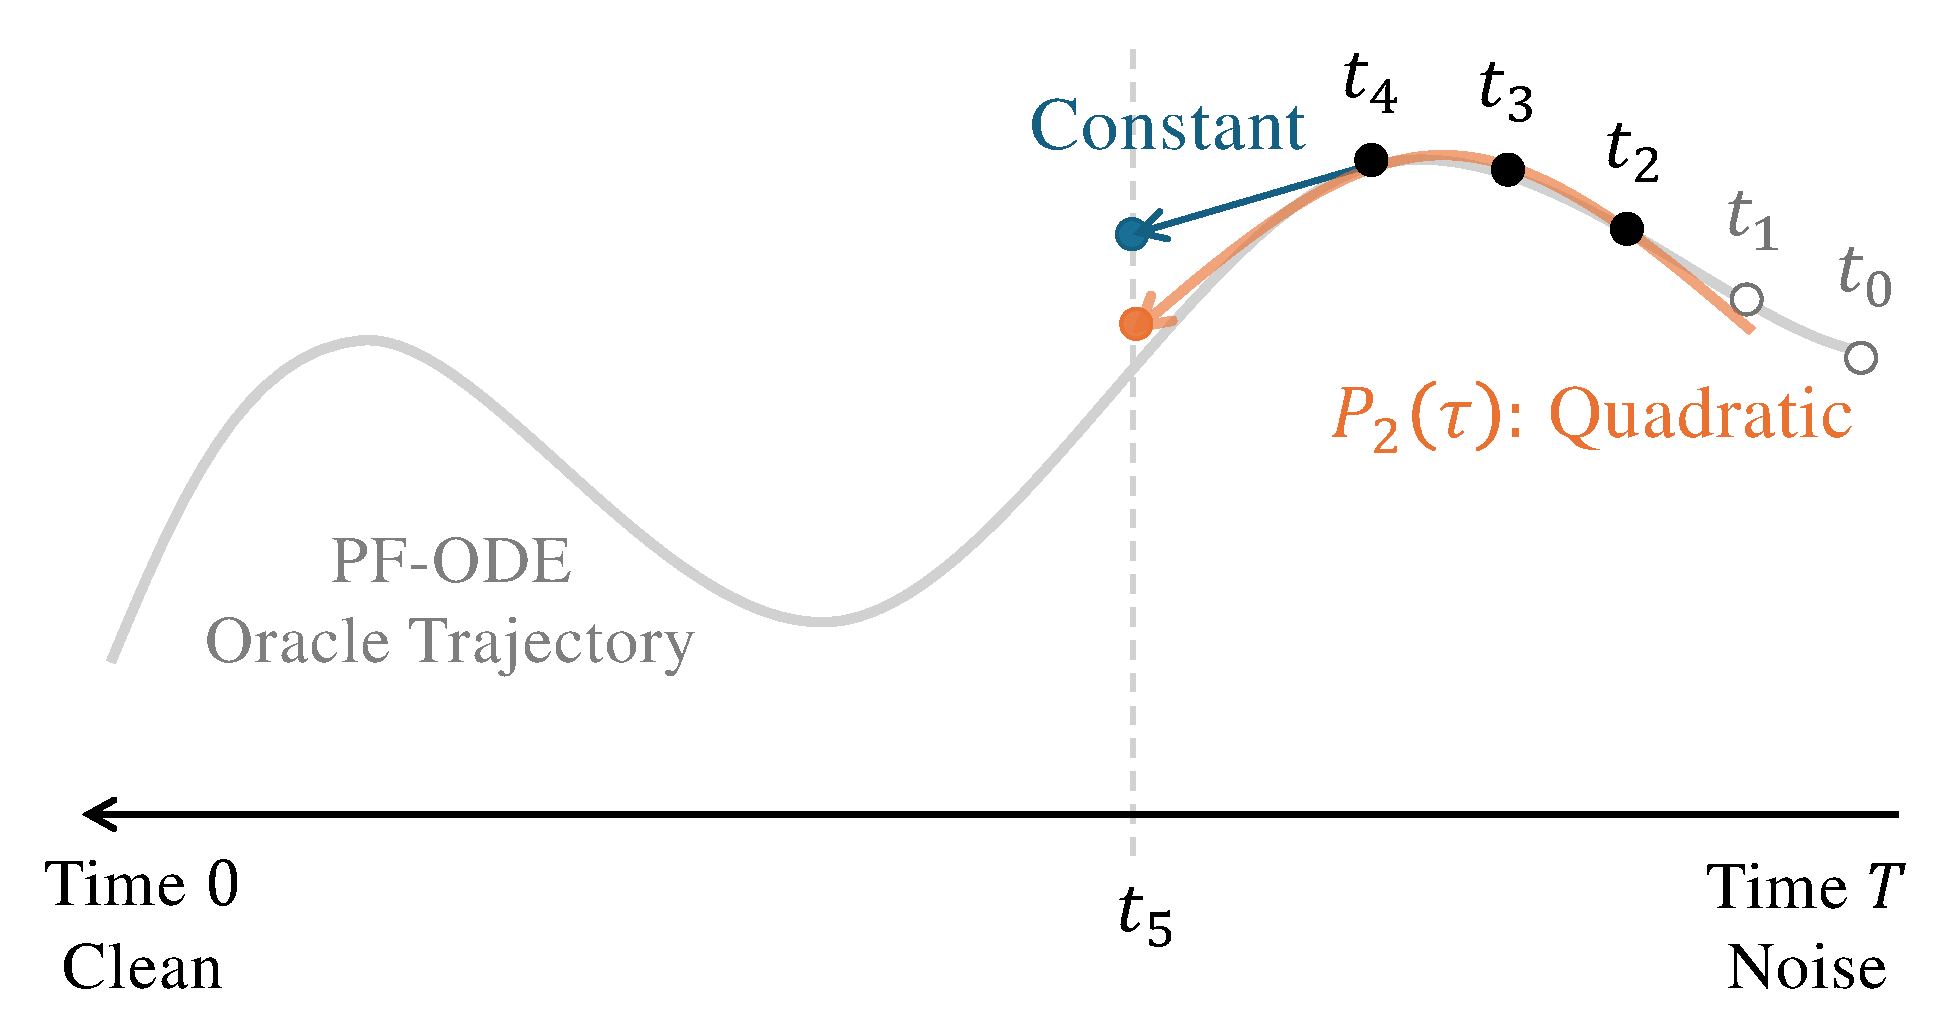
\includegraphics[width=\linewidth]{Images/PartC/DEIS.pdf}
    \caption{\textbfs{将 DEIS 视为多步方法的示意图。} 借助
$t_2,t_3,t_4$ 处的三个过去锚点，DEIS 通过模型输出构造一条二次曲线，
并对其解析积分以从
$t_4$ 步进到 $t_5$（外推）。这种高阶更新相比
DDIM 等一阶方法（仅使用 $t_4$ 处的值作积分的常数近似）减少了离散化误差。
\figcredit{由作者绘制。}}
    \label{fig:deis_lagrange}
\end{figure}

$n$ 次更新需要 $n{+}1$ 个锚点。当它们可用时（\emph{历史充分}，$i \ge n{+}1$），我们使用完整的 $n$ 次格式。在早期步骤中（\emph{历史不足}，$i \le n$），我们在可实现的最高次数 $i{-}1$ 上应用相同的构造，并随着更多锚点的累积而提高次数。下面我们依次处理这两种情形。



\paragraph{情形一：$i = n+1,\dots,M$（历史充分）。}
DEIS 不只依赖最近的估计
$\bm{\epsilon}_{\bm{\phi}^\times}(\tilde{\rvx}_{t_{i-1}},t_{i-1})$，
而是复用最后 $n{+}1$ 次模型求值作为锚点，
\[
(\tau_j,\rmY_j) := \bigl(t_{i-1-j}, \bm{\epsilon}_{\bm{\phi}^\times}(\tilde{\rvx}_{t_{i-1-j}},t_{i-1-j})\bigr),
\quad j=0,\dots,n.
\]
作为锚点。把 $\tau\mapsto\bm{\epsilon}_{\bm{\phi}^\times}(\rvx_\tau,\tau)$ 视为沿轨迹的光滑时间函数，我们构造 $n$ 次多项式（Lagrange 插值）
\[
P_n(\tau)
= 
\sum_{j=0}^{n}
\underbrace{\Bigl[\prod_{\substack{k=0\\k\neq j}}^{n}
\frac{\tau - t_{i-1-k}}{\,t_{i-1-j} - t_{i-1-k}\,}\Bigr]}_{=:~\ell_j^{(i)}(\tau)}
\bm{\epsilon}_{\bm{\phi}^\times}\bigl(\tilde{\mathbf x}_{t_{i-1-j}}, t_{i-1-j}\bigr)
\]
按构造它对每个锚点满足 $P_n(\tau_j)=\rmY_j$：
\[
P_n\bigl(\tau_j\bigr)
= \rmY_j =
\bm{\epsilon}_{\bm{\phi}^\times}\bigl(\tilde{\mathbf x}_{t_{i-1-j}}, t_{i-1-j}\bigr),
\quad
 j=0,\ldots,n.
\]
每个 $\ell_j^{(i)}$ 满足
\[
\ell_j^{(i)}\bigl(t_{i-1-m}\bigr)
=
\begin{cases}
1,&m=j,\\
0,&m\neq j.
\end{cases}
\]

Lagrange 多项式在新步上提供光滑外推：
\[
\bm{\epsilon}_{\bm{\phi}^\times}(\rvx_\tau,\tau) \approx
P_n(\tau)=\sum_{j=0}^{n}\ell_j^{(i)}(\tau) 
\bm{\epsilon}_{\bm{\phi}^\times}\bigl(\tilde{\rvx}_{t_{i-1-j}}, t_{i-1-j}\bigr), 
\quad \tau \in [t_{i-1},t_i].
\]
然后我们将 $P_r(\tau)$ 代入
指数积分器公式（\Cref{eq:variation_of_constants}）中 $\beps_{\bm{\phi}^\times}(\rvx_\tau,\tau)$ 的位置：
\begin{align*}
    \int_{t_{i-1}}^{t_i}
\frac{g^2(\tau)}{2 \sigma_\tau} 
\mathcal{E}&(\tau\to t_i) 
\beps_{\bm{\phi}^\times}(\rvx_\tau,\tau)\diff\tau
\\&\approx\sum_{j=0}^{r}
\underbrace{\int_{t_{i-1}}^{t_i}
\frac{g^2(\tau)}{2 \sigma_\tau} 
\mathcal{E}(\tau\to t_i) 
\ell_j^{(i)}(\tau)\diff\tau}_{=:~C_{i,j}} 
\beps_{\bm{\phi}^\times}(\tilde{\rvx}_{t_{i-1-j}},t_{i-1-j}).
\end{align*}
权重 $C_{i,j}$ 由
\begin{equation*}
C_{i,j} := \frac{1}{2} \int_{t_{i-1}}^{t_i} \frac{g^2(\tau)}{\sigma_\tau} \mathcal{E}(\tau \to t_i) \ell_j^{(i)}(\tau) \diff\tau,
\end{equation*}
给出，仅依赖于调度 $(\alpha_\tau,\sigma_\tau)$ 和网格
$\{t_i\}$。因此，一旦步长固定，它们就可以闭式地精确预计算。

用 $\mathcal{E}(t_{i-1}\to t_i)$ 精确积分线性部分，得到 \emph{AB-DEIS-$r$} 更新规则\footnote{“AB”指经典的
Adams–Bashforth 家族与指数时间差分多步方法~\citep{hochbruck2010exponential}。}，
\[
\tilde{\rvx}_{t_i}
=
\mathcal{E}(t_{i-1}\to t_i) \tilde{\rvx}_{t_{i-1}}
+
\sum_{j=0}^{r} C_{i,j} 
\beps_{\bm{\phi}^\times}(\tilde{\rvx}_{t_{i-1-j}},t_{i-1-j}).
\]
它在标准光滑性假设下给出 $r{+}1$ 阶的局部截断
误差.




\paragraph{情形二：$i=1,\dots,n$（历史不足）。}
对最初的若干步，只有 $i$ 个过去的点可用。因此我们把次数设为 $i{-}1$，并定义
\[
P_{i-1}(\tau)
=
\sum_{j=0}^{i-1}
\ell_j^{(i)}(\tau) 
\bm{\epsilon}_{\bm{\phi}^\times}\bigl(\tilde{\mathbf x}_{t_{i-1-j}},  t_{i-1-j}\bigr),
\]
其中 $\ell_j^{(i)}$ 是建立在时刻
$\{t_{i-1}, t_{i-2},\ldots,t_{0}\}$ 节点上的 $i{-}1$ 次 Lagrange 基。这匹配所有可用锚点，
并在 $i\ge n{+}1$ 时无缝过渡到完整历史公式。

这是多步求解器中标准的“热启动”。当历史较短时，我们拟合数据所允许的最丰富多项式：有一个锚点（$i{=}1$）时用 $0$ 次（常数）；有两个锚点（$i{=}2$）时用 $1$ 次（线性）；有三个锚点（$i{=}3$）时用 $2$ 次（二次）；以此类推，直到达到目标次数 $n$。实际上，随着更多历史可用，我们从单步预测逐步过渡到真正的 $(n{+}1)$ 步预测。


\exm{Lagrange 多项式的特例}{
\noindent \textbfs{当 $r=0$（一个锚点）：}
\[
P_0(\tau) = \bm{\epsilon}_{\bm{\phi}^\times}(\tilde\rvx_{t_{i-1}}, t_{i-1}).
\]
这只使用最近的值，因此近似在 $\tau$ 上是平坦的。
它对应于被积函数的左端点。

\medskip
\noindent \textbfs{当 $r=1$（两个锚点）：}Lagrange 多项式是穿过两个预先指定锚点的线性映射。
\[
P_1(\tau)
= 
\underbrace{\frac{\tau - t_{i-2}}{t_{i-1} - t_{i-2}}}_{\displaystyle \ell_{i-1}(\tau)}
\,\bm{\epsilon}_{\bm{\phi}^\times}(\tilde\rvx_{t_{i-1}}, t_{i-1})
 + 
\underbrace{\frac{\tau - t_{i-1}}{t_{i-2} - t_{i-1}}}_{\displaystyle \ell_{i-2}(\tau)}
\,\bm{\epsilon}_{\bm{\phi}^\times}(\tilde\rvx_{t_{i-2}}, t_{i-2}).
\]
这里 $\ell_{i-1}(\tau)$ 和 $\ell_{i-2}(\tau)$ 是 Lagrange 基权重。
它们满足插值（节点）条件
$P_1(t_{i-1})=\bm{\epsilon}_{\bm{\phi}^\times}(\tilde\rvx_{t_{i-1}}, t_{i-1})$ 与
$P_1(t_{i-2})=\bm{\epsilon}_{\bm{\phi}^\times}(\tilde\rvx_{t_{i-2}}, t_{i-2})$，
并且
$\ell_{i-1}(\tau)+\ell_{i-2}(\tau)=1$。
}

\paragraph{AB-DEIS-$n$ 更新总结。}
将历史充分与热启动（历史不足）两种情形合并，得到
\emph{AB-DEIS-$n$} 更新\footnote{“AB”指 Adams–Bashforth 家族的指数
时间差分多步方法~\citep{hochbruck2010exponential}。}，其中 $n$ 为多项式
次数（最多使用 $n{+}1$ 次过去的求值），如下：
\begin{mdframed}
\begin{align*}
\tilde\rvx_{t_i}
= \mathcal{E}(t_{i-1} \to t_i)\,\tilde\rvx_{t_{i-1}}
+ \sum_{j=0}^{\min\{n,\, i-1\}} C_{i,j}\,\beps_{\bm{\phi}^\times}(\tilde\rvx_{t_{i-1-j}},\,t_{i-1-j}),
\end{align*}
系数为
\begin{align*}
C_{i,j}
:= \frac{1}{2} \int_{t_{i-1}}^{t_i}
\frac{g^2(\tau)}{\sigma_\tau}\,\mathcal{E}(\tau \to t_i)\,
\Bigg[\prod_{\substack{k=0\\k\neq j}}^{\min\{n,\, i-1\}}
\frac{\tau - t_{i-1-k}}{\,t_{i-1-j} - t_{i-1-k}\,}\Bigg]\,d\tau.
\end{align*}
\end{mdframed}

当 $i\ge n{+}1$（历史充分）时，$\min\{n,\, i-1\}=n$
，在标准光滑性假设下该步达到局部截断误差 $\mathcal O(h^{\,n+1})$。
在热启动期间（$i\le n$），$\min\{n,\, i-1\}=i-1$，每步阶数为 $\mathcal O(h^{\,\min\{n,\, i-1\}+1})$，逐步爬升
直到达到完整阶数。

然而，非常大的 $n$ 往往由于插值病态、噪声放大以及更严格的稳定性约束而损害性能；小次数（例如 $n \in \{1,2,3\}$）通常提供最佳的精度—稳定性折中。

正如下一小节将看到的，$n{=}0$ 的特殊情形退化为指数 Euler/DDIM。



\subsection{DDIM = AB-DEIS-0}\label{sec:ddim-deis} 我们观察到，当 $ n = 0 $（即常数多项式）时，系数简化为：
\[
C_{i0} = \frac{1}{2} \int_{t_{i-1}}^{t_{i}} \frac{g^2(\tau)}{\sigma_\tau} \mathcal{E}(\tau \shortrightarrow t_i)   \mathrm{d}\tau.
\]
代入更新公式得到零阶 AB-DEIS 格式：
\begin{align}\label{eq:deis-0}
  \tilde\rvx_{t_{i}} &=  \mathcal{E}(t_{i-1} \shortrightarrow t_{i})\tilde\rvx_{t_{i-1}} + C_{i0} \bm{\epsilon}_{\bm{\phi}^\times}(\tilde\rvx_{t_{i-1}}, t_{i-1})\nonumber\\
  &=e^{\int_{t_{i-1}}^{t_{i}}f(u)\diff u} \tilde\rvx_{t_{i-1}} + \Big( \int_{t_{i-1}}^{t_{i}} \frac{g^2(\tau)}{2\sigma_\tau} e^{\int_{\tau}^{t_{i}}f(u)\diff u}   \mathrm{d}\tau
\Big) \bm{\epsilon}_{\bm{\phi}^\times}(\tilde\rvx_{t_{i-1}}, t_{i-1}).  
\end{align}
这正是指数 Euler 步（$[t_{i-1},t_i]$ 上 $\beps_{\bphi^\times}$ 为时间常数），与
确定性 DDIM 更新一致。我们在下面正式陈述这一对应关系。
\proppnp{DDIM = AB-DEIS-0}{ddim-deis}{\Cref{eq:deis-0} 与 \Cref{eq:ddim-euler} 中的 DDIM 更新完全相同。}


    
\clearpage
\newpage



\section{\texorpdfstring{DPM-Solver}{DPM-Solver}}\label{sec:dpm}

DPM-Solver 家族，包括 DPM-Solver~\citep{lu2022dpm}、DPM-Solver\texttt{++}~\citep{lu2022dpm2} 和 DPM-Solver-v3~\citep{zheng2023dpm}，代表了 PF-ODE 求解器的一项重大进展。其目标很简单：以远更少的步数达到相当的样本质量。在实践中，这些方法把 DDIM 所需的步数从 $50$ 多步减少到约 $10$--$15$ 步，使生成更高效。此外，DPM-Solver\texttt{++} 和 DPM-Solver-v3 设计用于处理条件生成中的无分类器引导（CFG）（见 \Cref{sec:cfg}）。本节首先讲解核心的 DPM-Solver~\citep{lu2022dpm}；其扩展见 \Cref{sec:dpm++}。

\paragraph{DPM-Solver 的高层思想。}
与 DEIS 一样，DPM-Solver 从 PF-ODE 的半线性形式出发，在 $\beps$-预测参数化下工作，使用 \Cref{eq:exp-int-factor} 中的指数积分器（常数变易）表示：
\begin{align}\label{eq:noise-alpha-sigma}
    \frac{\diff \rvx_t}{\diff t}
= \frac{\alpha_t'}{\alpha_t}\rvx_t
- \sigma_t \left(\frac{\alpha_t'}{\alpha_t}-\frac{\sigma_t'}{\sigma_t}\right)
\beps_{\bphi^\times}(\rvx_t,t).
\end{align}
关键思想是用半对数信噪比重新参数化时间，使指数积分器公式中的非线性项变为一个指数加权的积分。这种表示允许在 $\lambda$ 中进行低成本的 Taylor 展开，自然地给出高阶更新规则。我们随后将直观解释为何这种重参数化有效。



\subsection{DPM-Solver 的洞见：通过 log-SNR 进行时间重参数化}\label{subsec:dpm-method}   
在半线性结构之上，DPM-Solver 的一个关键洞见是：标准的时间参数化 $t$ 对扩散模型的数值积分而言是次优的。他们转而提出用\emph{半对数信噪比}（half-log SNR）
\begin{align}\label{eq:lambda}
    \lambda_t \coloneqq \frac{1}{2}\log \frac{\alpha_t^2}{\sigma_t^2}  =  \log \frac{\alpha_t}{\sigma_t},
\end{align}
来重参数化时间，
沿用 VDM~\citep{kingma2021variational} 的 log-SNR 参数化。
这种换元简化了非线性被积函数，从而能够进行更易处理、更精确的高阶模型估计。






\paragraph{将 PF-ODE 换元到 log-SNR。} 现在我们用半对数 log-SNR $\lambda_t := \log(\alpha_t/\sigma_t)$ 重新参数化时间。
对常见的噪声调度，$\lambda_t$ 关于 $t$ 严格递减。在此假设下，它有反函数 $t_\lambda(\cdot)$ 把 $\lambda$ 映射到 $t$，满足
\[
t = t_\lambda(\lambda(t)).
\]
然后我们将 $\rvx$ 和 $\bm{\epsilon}_{\bm{\phi}^\times}$ 的下标由 $t$ 改为 $\lambda$。带帽子（  $\hat{\cdot}$  ）表示该量以 $\lambda$ 表示。更精确地，定义：
\begin{align}
\begin{aligned}
    \label{eq:change-of-var-x-epsilon}
 \hat{\rvx}_{\lambda} & := \rvx_{t_\lambda(\lambda)}, \\
 \hat{\bm{\epsilon}}_{\bm{\phi}^\times}(\hat{\rvx}_{\lambda}, \lambda) & \coloneqq \bm{\epsilon}_{\bm{\phi}^\times}(\rvx_{t_\lambda(\lambda)}, t_\lambda(\lambda)).
\end{aligned}
\end{align}

通过从 $t$ 到 $\lambda_t$ 的换元，\Cref{eq:noise-alpha-sigma} 中 PF-ODE 的精确解 $\widetilde\bPsi_{s\to t}$ 变为：
\proppp{指数加权的精确解}{exp-wgt-exact-sol}{给定时刻 $s>0$ 的初值 $\rvx_s$，PF-ODE 在时刻 $t\in[0,s]$ 的精确解 $\widetilde\bPsi_{s\to t}(\rvx_s)$ 可以重新表示为：
\begin{equation}
\label{eq:analytic_solution}
    \widetilde\bPsi_{s\to t}(\rvx_s) = \frac{\alpha_t}{\alpha_s}\rvx_s - \alpha_t \int_{\lambda_s}^{\lambda_t} e^{-\lambda} \hat{\bm{\epsilon}}_{\bm{\phi}^\times}(\hat\rvx_\lambda,\lambda)\diff \lambda.
\end{equation}}{虽然可以直接对 \Cref{eq:noise-alpha-sigma} 施加换元得到结果，但为了清晰与完整，下面给出另一种推导。
利用关系 $ g^2(t) = -2\sigma_t^2\frac{\diff \lambda_t}{\diff t} $，\Cref{eq:noise-alpha-sigma} 可改写为：
\[
\frac{\diff \rvx_t}{\diff t} = \frac{\diff \log \alpha_t}{\diff t} \rvx_t - \sigma_t \frac{\diff \lambda_t}{\diff t} \bm{\epsilon}_{\bm{\phi}^\times}(\rvx_t, t).
\]
应用链式法则：
\[
\frac{\diff \rvx_t}{\diff t} = \frac{\diff \hat\rvx_\lambda}{\diff \lambda} \frac{\diff \lambda_t}{\diff t} \quad \text{and} \quad \frac{\diff \log\alpha_t}{\diff t} = \frac{\diff \log\alpha_\lambda}{\diff \lambda} \frac{\diff \lambda_t}{\diff t},
\]
$t $ 中的 ODE 变换为 $ \lambda $ 中的 ODE：
\begin{align*}
    \frac{\diff \hat\rvx_\lambda}{\diff \lambda} &= \Big(\frac{\diff \lambda_t}{\diff t}\Big)^{-1} \frac{\diff \rvx_t}{\diff t} \\
    &= \Big(\frac{\diff \lambda_t}{\diff t}\Big)^{-1} \Big[ \frac{\diff \log \alpha_t}{\diff t} \rvx_t - \sigma_t \frac{\diff \lambda_t}{\diff t} \bm{\epsilon}_{\bm{\phi}^\times}(\rvx_t, t) \Big] \\
    &= \Big(\frac{\diff \lambda_t}{\diff t}\Big)^{-1} \Big[ \frac{\diff \log\alpha_\lambda}{\diff \lambda} \frac{\diff \lambda_t}{\diff t} \hat\rvx_\lambda - \sigma_\lambda \frac{\diff \lambda_t}{\diff t} \hat{\bm{\epsilon}}_{\bm{\phi}^\times}(\hat\rvx_\lambda, \lambda) \Big] \\
    &= \frac{\diff \log\alpha_\lambda}{\diff \lambda} \hat\rvx_\lambda - \sigma_\lambda \hat{\bm{\epsilon}}_{\bm{\phi}^\times}(\hat\rvx_\lambda, \lambda).
\end{align*}
于是，变换后的 ODE 变为 \Cref{eq:diffusion_ode_lambda_eps}。然后我们可对 \Cref{eq:diffusion_ode_lambda_eps} 施加同样的“指数积分器（EI）”技术来推导 \Cref{eq:analytic_solution}。
}

在 $\lambda$--时间下，模型出现在一个指数加权的积分中，
\[
\int_{\lambda_s}^{\lambda_t} e^{-\lambda} \hat{\bm{\epsilon}}_{\bm{\phi}^\times}(\hat\rvx_\lambda,\lambda) \diff \lambda,
\]
其中 $e^{-\lambda}$ 因子产生闭式系数并使被积函数变平滑，这正是高阶局部近似所需要的。

等价地，从 $t$ 到 $\lambda$ 的换元把 PF-ODE 变换为如下的微分形式（见上一命题中的推导）：
\begin{mdframed}
\begin{align}\label{eq:diffusion_ode_lambda_eps}
\frac{\diff \hat{\rvx}_\lambda}{\diff \lambda}
= \frac{\alpha_\lambda'}{\alpha_\lambda} \hat{\rvx}_\lambda
- \sigma_\lambda \hat{\bm{\epsilon}}_{\bm{\phi}^\times}(\hat{\rvx}_\lambda, \lambda).
\end{align}
\end{mdframed}


\paragraph{为何要重参数化时间的直观理解？}
对严格单调的 $\lambda(t)$，一阶换元给出
\[
\Delta t  \approx  \frac{\Delta\lambda}{ |\lambda'(t)| }.
\]
因此，对固定的 $\Delta\lambda$，所诱导的 $\Delta t$ 在 $|\lambda'(t)|$ 较大处（即 $\lambda$ 随 $t$ 快速变化处）更小，在 $|\lambda'(t)|$ 较小处更大。
这种重参数化并不改变 PF--ODE 的解路径，只改变速度：
\[
\frac{\diff \hat\rvx_\lambda}{\diff \lambda}
= \frac{1}{\lambda'(t)} \frac{\diff \rvx_t}{\diff t}.
\]
于是，在 $|\lambda'(t)|$ 大的区域，$\lambda$--域导数被 $1/|\lambda'(t)|$ 缩放，往往使被积函数在均匀 $\lambda$ 网格上更平滑。
（大 $|\lambda'(t)|$ 的精确位置取决于所选调度。）

从概念上讲，我们可能希望在过程接近复杂（数据）分布时分配更多的时间步。下面两个简单的调度示例说明了这种效应：
\begin{itemize}
\item $(\alpha_t,\sigma_t)=(1-t, t)$：这对应 FM 调度器。则
\[
\lambda(t)=\log\frac{1-t}{t},\quad 
\lambda'(t)=-\frac{1}{t(1-t)},\quad
\Delta t \approx \Delta\lambda   t(1-t).
\]
因此步长在两端（$t\to 0,1$）附近很小，在中间时刻附近最大。

\item $(\alpha_t,\sigma_t)=(1, t)$：这是 EDM 调度器~\citep{karras2022elucidating}，在 \Cref{sec:edm} 中介绍。若直接取自变量为噪声水平 $t=\sigma_t$，则
\[
\lambda(t)=\log\frac{1}{t},\quad 
\lambda'(t)=-\frac{1}{t},\quad
\Delta t \approx \Delta\lambda   t.
\]
$\lambda$ 中的均匀间距对应 $t$ 中的几何间距，或等价地对应方差中的几何间距（在小 $t$/高 SNR 处有大量小步，在大 $t$ 处更粗糙）。
\end{itemize}




\subsection{用 Taylor 展开估计积分}\label{subsec:dpm-method-2} 
DEIS 通过对跨先前求值的被积函数作多项式
插值来近似该指数加权积分（一种多步
方法）。DPM-Solver 从相同的精确积分表述出发，
但用 log-SNR 变量~$\lambda$ 重参数化时间，并通过在~$\lambda$ 中的局部 Taylor 展开（在每步内使用中间分阶段的求值）来导出
高阶更新（一种单步
方法）。后续的 DPM-Solver 多步变体与 DEIS 基于插值的视角联系更紧密，我们将在 \Cref{sec:summary-solver} 中回到这一比较。现在我们给出 DPM-Solver 的单步推导。



由 \Cref{eq:analytic_solution}，从时刻 $s$ 的前一个点 $\tilde\rvx_{s}$ 出发，时刻 $t$ 的解 $\tilde\rvx_{t} $ 为
\begin{equation}
\label{eqn:analytic_solution_each_step}
    \tilde\rvx_{t}  = \frac{\alpha_{t}}{\alpha_{s}} \tilde\rvx_{s} - \alpha_{t} \int_{\lambda_{s}}^{\lambda_{t}} e^{-\lambda} \hat{\bm{\epsilon}}_{\bm{\phi}^\times}(\hat\rvx_{\lambda}, \lambda)\diff\lambda.
\end{equation}
因此，我们需要近似如下形式的积分：
\begin{align*}
    \int_{\lambda_{s}}^{\lambda_{t}} e^{-\lambda} \hat{\bm{\epsilon}}_{\bm{\phi}^\times}(\hat\rvx_{\lambda}, \lambda)\diff\lambda.
\end{align*}

在区间 $\lambda \in [\lambda_{s}, \lambda_{t_i}]$ 上，我们对 \Cref{eqn:analytic_solution_each_step} 中的被积函数 $\hat{\bm{\epsilon}}_{\bm{\phi}^\times}(\hat\rvx_\lambda, \lambda)$ 用关于 $\lambda$ 的 Taylor 展开来近似。对 $n \geq 1$，关于 $\lambda_{s}$ 的 $(n{-}1)$ 阶 Taylor 展开为
\begin{equation*}
    \hat{\bm{\epsilon}}_{\bm{\phi}^\times}(\hat\rvx_\lambda, \lambda)
    = \sum_{k=0}^{n-1} \frac{(\lambda - \lambda_{s})^k}{k!} 
    \hat{\bm{\epsilon}}_{\bm{\phi}^\times}^{(k)}(\hat\rvx_{\lambda_{s}}, \lambda_{s})
    + \mathcal{O}((\lambda - \lambda_{s})^n),
\end{equation*}
其中关于 $\lambda$ 的 $k$ 阶全导数记为
\[
\hat{\bm{\epsilon}}_{\bm{\phi}^\times}^{(k)}(\hat\rvx_\lambda, \lambda) 
\coloneqq \frac{\diff^k}{\diff\lambda^k} \hat{\bm{\epsilon}}_{\bm{\phi}^\times}(\hat\rvx_\lambda, \lambda).
\]

将此展开代入 \Cref{eqn:analytic_solution_each_step} 中的积分，得到一个闭式近似，它定义了 $n$ 阶求解器，称为 \emph{DPM-Solver-$n$}。

\begin{mdframed}
从前一步的估计 $\tilde\rvx_{s}$ 出发，
\begin{equation}
    \label{eq:k-th-expansion}
    \tilde\rvx_{t}  =  \frac{\alpha_{t}}{\alpha_{s}} \tilde\rvx_{s} - \alpha_{t} \sum_{k=0}^{n-1} {\color{cyan}\hat{\bm{\epsilon}}_{\bm{\phi}^\times}^{(k)}(\hat\rvx_{\lambda_{s}},\lambda_{s})} ~{\color{orange}C_k}  + \mathcal{O}(h^{n+1}),
\end{equation}
这里记 $h\coloneqq \lambda_{t} - \lambda_{s}$，并定义：
\begin{align*}
    {\color{orange}C_k}\coloneqq\int_{\lambda_{s}}^{\lambda_{t}}   e^{-\lambda}  \frac{(\lambda - \lambda_{s})^k}{k!}\diff\lambda.
\end{align*}
${\color{orange}C_k}$ 可通过应用 $k$ 次分部积分解析地预计算。
\end{mdframed}
我们注意到，换元 $t \mapsto \lambda$ 用于
平滑被积函数并推导系数，而求解器
返回的是 $t$-网格上的估计 $\tilde{\rvx}_{t}$。

下面，我们以 DPM-Solver-1 为例说明。


\exm{DPM-Solver-1}{
为演示取 $n=1$（一阶）。从前一个估计点 $\tilde\rvx_{s}$ 出发，\Cref{eq:k-th-expansion} 简化为：
\begin{align}\label{eq:dpm-1}
    \tilde\rvx_{t} &= \frac{\alpha_{t}}{\alpha_{s}} \tilde\rvx_{s} - \alpha_{t} \bm{\epsilon}_{\bm{\phi}^\times}(\tilde\rvx_{s},s) \int_{\lambda_{s}}^{\lambda_{t}} e^{-\lambda}\diff\lambda + \mathcal{O}(h^2) \nonumber \\
    &= \frac{\alpha_{t}}{\alpha_{s}} \tilde\rvx_{s} - \sigma_{t} (e^{h} - 1)\bm{\epsilon}_{\bm{\phi}^\times}(\tilde\rvx_{s},s) + \mathcal{O}(h^2).   
    \end{align}
上式正是 DDIM 更新；我们在 Proposition~\ref{ddim-dpm} 中证明其等价性。
}

$n \ge 2$ 的 DPM-Solver-$n$ 需要对 $k \le n-1$ 求值 $k^{\text{th}}$ 阶导数 {\color{cyan}$\hat{\bm{\epsilon}}_{\bm{\phi}^\times}^{(k)}(\hat\rvx_\lambda, \lambda)$}。然而，在实践中直接计算高阶导数代价高昂。\citet{lu2022dpm} 也提出了这些导数的高效近似方法，将在下一小节详述。

 
\subsection{DPM-Solver-$n$ 的实现}\label{subsec:dpm-n-method} 

\paragraph{$n \ge 2$ 的 DPM-Solver-$n$。}
在实践中，实现高阶的 DPM-Solver-$n$ 包含以下内容：
\begin{itemize}
    \item 预计算系数 ${\color{orange}C_k}$；
    \item 近似 $k \le n-1$ 的 $k^{\text{th}}$ 阶导数 {\color{cyan}$\hat{\bm{\epsilon}}_{\bm{\phi}^\times}^{(k)}(\hat\rvx_\lambda,\lambda)$} 以规避昂贵的精确高阶导数计算——这是 ODE 文献中研究充分的一个挑战~\citep{hochbruck2005explicit,luan2021efficient}。一种常见策略是有限差分近似。
\end{itemize}

下面我们详细说明前两点。


\subparagraph{预计算 ${\color{orange}C_k}$。} 
设 $s$ 和 $t$ 分别表示起始和终止时刻，并定义 $h := \lambda_t - \lambda_s$。从 $\rvx_s$ 出发，\Cref{eq:variation_of_constants} 的精确解的解析展开为：
\begin{equation}
\label{eq:analytic_expansion}
    \rvx_{t} = \frac{\alpha_{t}}{\alpha_{s}}\rvx_{s} - \sigma_{t} \sum_{k=0}^{n-1} h^{k+1} \varphi_{k+1}(h) \hat{\bm{\epsilon}}_{\bm{\phi}^\times}^{(k)}(\hat\rvx_{\lambda_{s}}, \lambda_{s}) + \mathcal{O}(h^{n+1}),
\end{equation}
其中每个 $\varphi_{k+1}(\cdot)$ 有闭式表达。对 $k = 0, 1, 2$，它们为：
\begin{align*}
\varphi_1(h) &= \frac{e^h - 1}{h}, &
\varphi_2(h) &= \frac{e^h - h - 1}{h^2}, &
\varphi_3(h) &= \frac{e^h - \frac{h^2}{2} - h - 1}{h^3}.
\end{align*}

\exm{使用精确导数的 DPM-Solver-2/3}{对 $n = 3$ 及离散时间步 $h := \lambda_{t} - \lambda_{s}$，展开变为：
\begin{equation}\label{eq:example-dpm-solver-3-exact}
\begin{aligned}
    \rvx_{t} = \frac{\alpha_{t}}{\alpha_{s}} \rvx_{s}
    &- \sigma_{t} \left(e^{h} - 1\right) \hat{\bm{\epsilon}}_{\bm{\phi}^\times}(\hat\rvx_{\lambda_{s}}, \lambda_{s}) \\
    &- \sigma_{t} \left(e^{h} - h - 1\right) \hat{\bm{\epsilon}}_{\bm{\phi}^\times}^{(1)}(\hat\rvx_{\lambda_{s}}, \lambda_{s}) \\
    &- \sigma_{t} \left(e^{h} - \frac{h^2}{2} - h - 1\right) \hat{\bm{\epsilon}}_{\bm{\phi}^\times}^{(2)}(\hat\rvx_{\lambda_{s}}, \lambda_{s}) \\
    &+ \mathcal{O}(h^4).
\end{aligned}
\end{equation}}





\subparagraph{近似 $k \le n-1$ 的 {\color{cyan}$\hat{\bm{\epsilon}}_{\bm{\phi}^\times}^{(k)}(\hat\rvx_\lambda,\lambda)$}。}
对 $n \ge 2$，遵循单步 ODE 求解器的标准方法~\citep{atkinson2009numerical}，\citet{lu2022dpm} 在 $s$ 和 $t$ 之间引入中间时间步 $s^{\mathrm{mid}}$，用 $s$ 和 $s^{\mathrm{mid}}$ 处的函数求值来近似高阶导数。我们以 $n = 2$ 的情形为例说明。

设 $\gamma \in (0,1]$ 为指定 log-SNR 区间 $[\lambda_s, \lambda_t]$ 内一个插值点的超参数。
给定 $s$ 处的估计 $\tilde\rvx_s$，定义
\[
    s^{\mathrm{mid}} = t_\lambda\left(\lambda_s + \gamma h\right), \quad \text{where } h := \lambda_t - \lambda_s,
\]
中间估计由下式给出：
\[
    \rvx^{\mathrm{mid}} = \frac{\alpha_{s^{\mathrm{mid}}}}{\alpha_s} \tilde\rvx_s - \sigma_{s^{\mathrm{mid}}} \left(e^{\gamma h} - 1\right) \bm{\epsilon}_{\bm{\phi}^\times}(\tilde\rvx_s, s).
\]
这给出如下二阶近似：
\begin{align}
\label{eq:dpm-solver-2-app}
\begin{aligned}
    \tilde{\rvx}_{t} = \frac{\alpha_{t}}{\alpha_s} \tilde\rvx_s 
    &- \sigma_{t} \left(e^{h} - 1\right) \bm{\epsilon}_{\bm{\phi}^\times}(\tilde\rvx_s, s) \\
    &- \frac{\sigma_t}{\gamma h} \left(e^{h} - h - 1\right) \left( \bm{\epsilon}_{\bm{\phi}^\times}(\rvx^{\mathrm{mid}}, s^{\mathrm{mid}}) - \bm{\epsilon}_{\bm{\phi}^\times}(\tilde\rvx_s, s) \right)
     +  \mathcal{O}(h^3).
\end{aligned}
\end{align}


取 $\gamma=\tfrac12$ 时，\Cref{alg:dpm-solver-2} 中的两阶段更新在相差 $\mathcal O(h^3)$（局部截断误差）的意义下等价于
\Cref{eq:dpm-solver-2-app}。
\begin{algorithm}[H]
    \centering
    \caption{DPM-Solver-2（取 $\gamma=\tfrac12$）。}\label{alg:dpm-solver-2}
    \begin{algorithmic}[1]
    \Require 初值 $\rvx_T$，时间步 $\{t_i\}_{i=0}^M$，模型 ${\bm{\epsilon}}_{\bm{\phi}^\times}$
        \State $\tilde\rvx_{t_0}\gets\rvx_T$
        \For{$i\gets 1$ to $M$}
        \State $h_i \gets \lambda_{t_i} - \lambda_{t_{i-1}}$
        \State $s_{i}^{\text{mid}} \gets t_{\lambda}\left(\tfrac{\lambda_{t_{i-1}} + \lambda_{t_i}}{2}\right)$
        \State 
    $\rvx_{i}^{\text{mid}} \gets \tfrac{\alpha_{s_i^{\text{mid}}}}{\alpha_{t_{i-1}}} \tilde\rvx_{t_{i-1}} - \sigma_{s_i^{\text{mid}}}\left(e^{\tfrac{h_i}{2}} - 1\right){\bm{\epsilon}}_{\bm{\phi}^\times}(\tilde \rvx_{t_{i-1}},t_{i-1})$ 
    \State  $\tilde\rvx_{t_{i}} \gets \tfrac{\alpha_{t_{i}}}{\alpha_{t_{i-1}}} \tilde\rvx_{t_{i-1}} - \sigma_{t_{i}}\left(e^{h_i} - 1\right){\bm{\epsilon}}_{\bm{\phi}^\times}(\rvx_{i}^{\text{mid}},s_i^{\text{mid}})$
        \EndFor
        \State \Return $\tilde\rvx_{t_M}$
    \end{algorithmic}
\end{algorithm}

\rmkb{
在 \Cref{eq:dpm-solver-2-app} 中，差商
\[
\hat{\bm{\epsilon}}_{\bm{\phi}^\times}^{(1)}(\hat\rvx_{\lambda_s},\lambda_s)
\approx
\frac{\bm{\epsilon}_{\bm{\phi}^\times}(\rvx^{\mathrm{mid}}, s^{\mathrm{mid}})
      - \bm{\epsilon}_{\bm{\phi}^\times}(\tilde\rvx_s, s)}{\gamma h}
\]
近似了模型沿轨迹的 $\lambda$ 全导数。
此近似精确到 $\mathcal O(h)$，而在 \Cref{eq:dpm-solver-2-app} 中它乘以了精确的 $\varphi_2$ 系数 $e^h-h-1=\mathcal O(h^2)$。
因此，所得贡献仅为 $\mathcal O(h^3)$，所以对任意 $\gamma \in (0,1]$ 整个格式都达到二阶精度。

每步恰好需要两次模型求值：一次在 $(\tilde\rvx_s,s)$，另一次在预测的中点 $(\rvx^{\mathrm{mid}},s^{\mathrm{mid}})$。
插值参数 $\gamma$ 不影响精度阶，但它改变误差常数：取 $\gamma=\tfrac12$ 会使模板对称化，通常能最小化常数，这也是实践中偏好中点版本的原因。

}


对 $n \ge 3$ 的高阶 DPM-Solver-$n$，采用类似的方法，利用中间时间步以有限差分方式近似高阶导数。详细方法见原始 DPM 论文。


对熟悉数值 ODE 求解器的读者，\textsc{DPM-Solver} 可以被视为半线性 PF-ODE 的单步\emph{指数积分器}，并结合了到（半）log--SNR 的时间变量替换。其二阶与三阶变体是指数 Runge--Kutta 型格式，在每步内使用少量分阶段的模型求值。


\paragraph{实现细节：采样时间步的选择。} 为进行采样，求解器必须首先预定义一时间步序列 $\{t_i\}_{i=0}^M$。
\citet{lu2022dpm} 提出基于在 log--SNR 时间 $\lambda_t$ 中\emph{均匀间距}来选择这些步，即
\[
\lambda_{t_i} = \lambda_T + \frac{i}{M}(\lambda_0 - \lambda_T), \quad i = 0, \dots, M.
\]
这不同于早前方法~\citep{ho2020denoising,song2020score} 直接在物理时间变量~$t$ 中使用均匀间距的做法。
经验上，DPM-Solver 在使用均匀 $\lambda$ 间距时，即使步数很少也能得到高质量样本\footnote{或者，自适应步长策略通过组合不同阶数的求解器来动态调整时间步；见 \citet{lu2022dpm} 的附录 C。}。

从概念上讲，这可以从几何角度理解：局部 Taylor 近似的精度取决于动力学在 $\lambda$ 中演化的光滑程度。
因此 $\lambda$ 中的均匀间距在轨迹上产生近似均匀的局部误差，使得在信号主导（高 SNR）处有更细（更密）的 $t$ 步，在噪声主导的情形下有更粗（更稀）的步。



虽然推导在 $\lambda$--空间中进行，且 PF--ODE 在该域中表述为方便的半线性形式，但预训练模型和噪声调度 $(\alpha_t, \sigma_t)$ 通常相对于原始时间变量 $t$ 定义。
在采样过程中，求解器为数值稳定性选取在 $\lambda$ 中均匀间距的节点，但所有更新方程都以 $t$ 表达。
每当需要求值模型或检索调度值时，所选的 $\lambda$ 节点被映射回相应的时间变量，如物理时间 $t = t_\lambda(\lambda)$ 或方差参数 $\sigma_t$，具体取决于模型的参数化方式（例如见 \Cref{alg:dpm-solver-2}）。








\subsection{DDIM $=$ DPM-Solver-1}\label{subsec:ddim=dpm-solver-1}
对固定的调度 $(\alpha_t,\sigma_t)$，DPM-Solver-1 步
与确定性 DDIM（$\eta=0$）更新一致，
与时间参数化（物理时间 $t$ 或 log--SNR 时间 $\lambda$）无关；
正式陈述见下。
\proppp{DDIM 即 DPM-Solver-1}{ddim-dpm}{
\Cref{eq:ddim-euler} 给出的 DDIM 更新规则，与 \Cref{eq:dpm-1} 给出的 DPM-Solver-1 更新规则相同。
}{
由 $\lambda$ 的定义，有
\begin{align}
    \frac{\sigma_s}{\alpha_s} = e^{-\lambda_s} \quad \text{and} \quad \frac{\sigma_t}{\alpha_t} = e^{-\lambda_t}.
\end{align}
将这些表达式连同 $h = \lambda_t - \lambda_s$ 代入 \Cref{eq:ddim-euler}，即恢复 \Cref{eq:dpm-1} 中的更新规则，完成等价性证明。
}
上述命题或许能解释为何 DDIM 优于 $t$-参数化下的传统 Euler 方法：它在更合适的 $\lambda$-重参数化下有效地利用了扩散 ODE 的半线性。


\rmkb{当 Score SDE 论文出现时，常用 Runge--Kutta（RK45）来求解 \Cref{eq:prob_ode_sub} 中的朴素 PF-ODE，但其漂移的半线性并未被利用。尽管 DPM-Solver-$k$（$k \geq 2$）与 Runge--Kutta 方法有关，但它通过时间重参数化明确地利用了这种半线性。这解释了为何 DPM-Solver 能以远更少的函数求值达到高阶精度，在保持高样本质量的同时把 DDIM 通常数百步的调度减少到约 $10$--$15$ 步。
}






\subsection{关于 DPM-Solver-2 与经典 Heun 更新的讨论}\label{subsec:dpm-heun}

在 \Cref{subsec:ddim-different-para} 中我们看到，PF--ODE 的不同参数化给出经典 Euler 型更新的不同解读：
\begin{align*}
\text{$\rvv$-prediction:} 
&\quad \text{Euler} = \text{DDIM}, \\[4pt]
\text{$\beps$-, $\rvx$-, or $\rvs$-prediction:} 
&\quad \text{exp--Euler} = \text{DDIM} \neq \text{plain Euler}.
\end{align*}

本小节我们进一步通过考察经典 \emph{Heun 方法}与二阶 DPM--Solver 在四种参数化下的类似关系来说明这一联系。


作为铺垫，我们简要回顾 Heun 方法（另见 \Cref{app:de-solver}）。
Heun 方法是一种二阶求解器，它通过预测器-校正器格式改进 Euler 方法：
它先做一次 Euler 预测到步的终点，在那里求值斜率，然后用
起点与预测斜率的平均进行更新。
直观上，它沿区间内的平均斜率前进
（梯形的面积），达到比朴素 Euler 高得多的精度。

我们在 log--SNR 时间 $\lambda$ 中工作，其中 PF--ODE 可表示为简单的“线性 + 非线性”形式：
\[
\frac{\diff \hat{\rvx}(\lambda)}{\diff \lambda}
= \underbrace{L(\lambda)\hat{\rvx}(\lambda)}_{\text{linear part}} + \underbrace{\rmN\big(\hat{\rvx}(\lambda),\lambda\big)}_{\text{nonlinear part}},
\]
其中标量 $L(\lambda)$ 由噪声调度决定，$\rmN(\cdot,\lambda)$ 收集非线性部分。
这种结构自然来自 \Cref{eq:clean_pf_ode}：$\beps$-、$\rvx$-和 $\rvs$-预测参数化给出非零 $L(\lambda)$，从而呈现半线性形式。
相比之下，$\rvv$-预测对应于 $L(\lambda)\equiv 0$（因此 $\rmN=\rvv$），不留下显式的线性项。


在下文的讨论中，我们先回顾不考虑任何半线性结构的朴素 Heun 更新，
然后引入指数 Heun 更新——它专为半线性 ODE 设计并精确处理线性部分，类似于 \Cref{eq:exp-euler-step,eq:euler-step} 中的指数 Euler 步。
最后，我们将两种 Heun 更新与四种参数化下的 DPM-Solver-2 联系起来，并得出结论：
\begin{align*}
\text{$\rvv$-prediction:} 
&\quad \text{Heun} = \text{DPM-Solver-2}, \\[4pt]
\text{$\beps$-, $\rvx$-, or $\rvs$-prediction:} 
&\quad \text{exp-Heun} = \text{DPM-Solver-2} \neq \text{plain Heun}.
\end{align*}

\begin{figure}[th!]
    \centering
    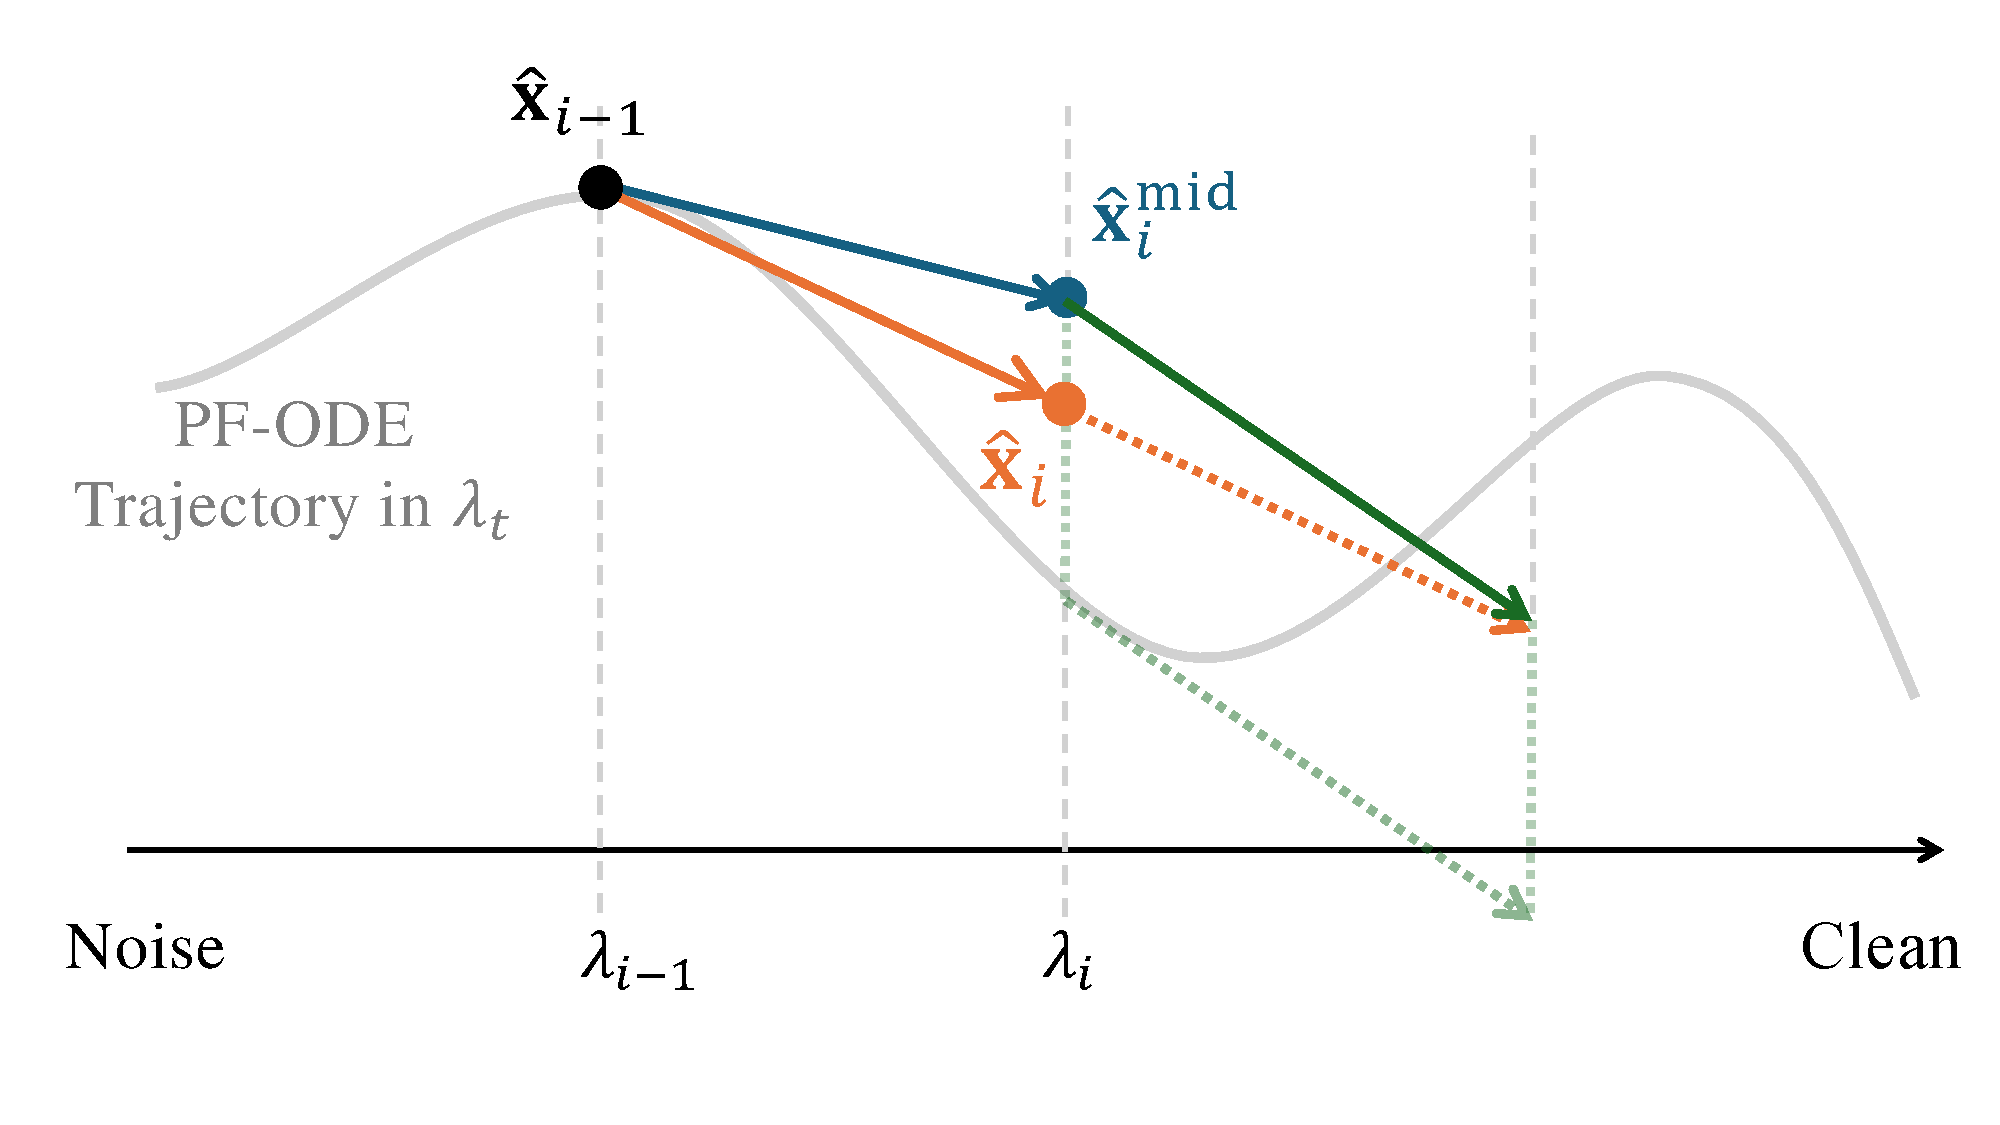
\includegraphics[width=\linewidth]{Images/PartC/Heun.pdf}
\caption{
\textbfs{log-SNR 时间中的朴素 Heun 更新。}
从前一状态 $\hat{\mathbf{x}}_{i-1}$（在 $\lambda_{i-1}$）出发，
\emph{预测器}步（蓝色箭头）执行一次显式 Euler 移动
$h \rmF(\hat{\mathbf{x}}_{i-1}, \lambda_{i-1})$ 以得到中间估计
$\hat{\mathbf{x}}^{\mathrm{mid}}_i$。
在该预测点，\emph{校正器}步求值新斜率
$h \rmF(\hat{\mathbf{x}}^{\mathrm{mid}}_i, \lambda_i)$（绿色箭头），并通过平行四边形构造组合两个斜率：
虚线橙色对角线表示从 $\hat\rvx_{i-1}$ 出发的向量求和
$h\big(\rmF(\hat{\rvx}_{i-1},\lambda_{i-1}) + \rmF(\hat{\rvx}^{\mathrm{mid}}_{i},\lambda_{i})\big)$，
实线橙色箭头是其半对角线，方向相同但长度减半。
这一过程实现了 log-SNR 时间下 PF-ODE 轨迹的朴素 Heun 积分。
\figcredit{由作者绘制。}
}
    \label{fig:plain-heun}
\end{figure}

\paragraph{朴素 Heun 更新。}
记 $\lambda_i:=\lambda_{t_i}$，则 $\{\lambda_i\}_{i=0}^M$ 是 log-SNR 域中的递增网格，并设 $h := \lambda_i - \lambda_{i-1} > 0$。
设 $\hat{\rvx}_{i-1}$ 为 log-SNR 时间中的前一个迭代点。
直接应用于完整漂移
\[
\rmF(\hat{\rvx}, \lambda) := L(\lambda) \hat{\rvx} + \rmN(\hat{\rvx}, \lambda),
\]
log-SNR 时间中的朴素 Heun 更新为
\begin{align}\label{eq:heun-logsnr}
\begin{aligned}
    \text{预测：}\quad 
&\hat{\rvx}^{\mathrm{mid}}_i 
= \hat{\rvx}_{i-1} + h \rmF(\hat{\rvx}_{i-1},\lambda_{i-1}),\\
\text{校正：}\quad 
&\hat{\rvx}_{i} 
= \hat{\rvx}_{i-1} + \tfrac{h}{2}\Big(\rmF(\hat{\rvx}_{i-1},\lambda_{i-1}) + \rmF(\hat{\rvx}^{\mathrm{mid}}_{i},\lambda_{i})\Big).
\end{aligned}
\end{align}

\paragraph{指数 Heun 更新（针对半线性 PF-ODE）。} 使用\emph{指数积分器}技术，其思想是对 ODE 的线性与非线性部分区别对待。
线性项 $L(\lambda)\hat{\rvx}$ 在该步上被精确积分，
而非线性项 $\rmN(\hat{\rvx},\lambda)$ 仅通过在该步上取平均来近似。

为简洁表达，我们引入量
\[
\mathcal{E} := \int_{\lambda_{i-1}}^{\lambda_{i}} L(\tau) \diff\tau,
\]
它表示线性系数 $L(\lambda)$ 在区间 $[\lambda_{i-1}, \lambda_i]$ 上的总贡献。
利用 $\mathcal{E}$，我们定义两个辅助系数 $c_1(\mathcal{E})$ 和 $c_2(\mathcal{E})$ 以同时处理两种
情形：$\mathcal{E}$ 非零以及 $\mathcal{E}$ 为零：
\[
c_1(\mathcal{E}) =
\begin{cases}
\tfrac{e^{\mathcal{E}} - 1}{\mathcal{E}}, & \text{if } \mathcal{E}\neq 0,\\[6pt]
1, & \text{if } \mathcal{E}=0,
\end{cases}
\qquad
c_2(\mathcal{E}) =
\begin{cases}
\tfrac{e^{\mathcal{E}} - 1 - \mathcal{E}}{\mathcal{E}^2}, & \text{if } \mathcal{E}\neq 0,\\[6pt]
\tfrac{1}{2}, & \text{if } \mathcal{E}=0.
\end{cases}
\]
第二种情形只是确保当线性项消失（$L(\lambda)=0$）时的连续性，使得公式仍然有效并光滑地退化为 \Cref{eq:heun-logsnr} 中的标准 Heun 更新。

有了这些系数，指数 Heun 格式的一个更新步可写为：
\begin{align}\label{eq:exp-heun-logsnr}
\begin{aligned}
    \text{预测：}\quad 
&\hat{\rvx}^{\mathrm{mid}}_{i} 
= e^{\mathcal{E}}\hat{\rvx}_{i-1} + h c_1(\mathcal{E}) \rmN(\hat{\rvx}_{i-1},\lambda_{i-1}),\\
\text{校正：}\quad 
&\hat{\rvx}_{i} 
= e^{\mathcal{E}}\hat{\rvx}_{i-1}
\begin{aligned}[t]
    &+ h c_1(\mathcal{E}) \rmN(\hat{\rvx}_{i-1},\lambda_{i-1})
\\&+ h c_2(\mathcal{E})\Big(\rmN(\hat{\rvx}^{\mathrm{mid}}_{i},\lambda_{i})-\rmN(\hat{\rvx}_{i-1},\lambda_{i-1})\Big).
\end{aligned}
\end{aligned}
\end{align}

当 $L(\lambda)\equiv 0$ 时，系数简化为 $c_1=1$ 和 $c_2=\tfrac{1}{2}$，方法退化为 \Cref{eq:heun-logsnr} 中的朴素 Heun 求解器。

当 $L(\lambda)\neq 0$ 时，更新的指数积分器形式精确积分线性项，
而朴素 Heun 方法仅提供近似。
为看清这一点，对小步长
$h = \lambda_i - \lambda_{i-1} > 0$ 展开指数项。
由于
\[
\mathcal{E} = \int_{\lambda_{i-1}}^{\lambda_i} L(\tau)\diff\tau 
= h L(\lambda_{i-1}) + \mathcal O(h^2),
\]
我们可把 $\mathcal{E}$ 视为 $\mathcal O(h)$ 阶的小量。Taylor 展开给出：
\[
e^{\mathcal{E}} = 1 + \mathcal{E} + \tfrac{\mathcal{E}^2}{2} + \mathcal O(\mathcal{E}^3),\,\,
c_1(\mathcal{E}) = 1 + \tfrac{\mathcal{E}}{2} + \tfrac{\mathcal{E}^2}{6} + \mathcal O(\mathcal{E}^3),\,\,
c_2(\mathcal{E}) = \tfrac{1}{2} + \tfrac{\mathcal{E}}{6} + \tfrac{\mathcal{E}^2}{24} + \mathcal O(\mathcal{E}^3).
\]

将这些近似代入 \Cref{eq:exp-heun-logsnr} 并保留到 $\mathcal{E}^2$ 项（即由于 $\mathcal{E}=\mathcal{O}(h)$ 而保留到 $h^2$ 阶），
更新恰好简化为朴素 Heun 形式（\Cref{eq:heun-logsnr}）。
两种格式之间的剩余差异仅出现在 $\mathcal{O}(\mathcal{E}^3)=\mathcal{O}(h^3)$ 阶的更高阶项中。
直观上，当步长 $h$ 很小时，$\mathcal{E}$ 也很小，所以指数因子
退化为
\[
e^{\mathcal{E}} \approx 1+\mathcal{E},\quad 
c_1(\mathcal{E}) \approx 1,\quad c_2(\mathcal{E}) \approx \tfrac{1}{2}.
\]
因此，“线性已处理”的指数 Heun 更新退化为朴素 Heun 步。

\paragraph{四种预测下 Heun 更新与 DPM--Solver-2 的联系。}
我们强调，在 PF-ODE 的 $\beps$-预测形式中（见 \Cref{eq:diffusion_ode_lambda_eps}），
log--SNR 时间 $\lambda$ 中的动力学自然呈现所需的半线性形式：
\[
\frac{\diff \hat{\rvx}_\lambda}{\diff \lambda}
= \underbrace{\frac{\alpha_\lambda'}{\alpha_\lambda}}_{=:L(\lambda)} \hat{\rvx}_\lambda
+
\underbrace{\big(- \sigma_\lambda \hat{\bm{\epsilon}}_{\bm{\phi}^\times}(\hat{\rvx}_\lambda,\lambda)\big)}_{=:\rmN(\hat{\rvx}_\lambda,\lambda)}.
\]
因此，对 log--SNR 时间 $\lambda$ 中的 $\beps$-预测，\Cref{eq:exp-heun-logsnr} 中的指数 Heun 更新
\emph{恰好等价于} DPM-Solver-2
（中点参数 $\gamma=\tfrac{1}{2}$；见 \Cref{alg:dpm-solver-2}）。

类似地，在 log--SNR 时间下的 $\rvx$-和 $\rvs$-预测参数化下，
它们的 PF-ODE 也呈现相同的半线性结构。
因此，$\beps$-、$\rvx$-或 $\rvs$-预测下的 DPM-Solver-2
与 \Cref{eq:exp-heun-logsnr} 中的指数 Heun 更新\emph{相同}。相比之下，$\rvv$-预测形式自然消去了线性项，
因此其 PF-ODE 不需要指数积分器；
log--SNR 时间中的朴素 Heun 方法已经提供了正确的二阶更新。

类似于 DDIM 中 Euler 与指数 Euler 的情形，我们因此得出如下结论： \msg{观察}{Heun 与 DPM-Solver-2 更新}{
给定 log-SNR 时间 $\lambda$ 中的 PF-ODE，
\begin{align*}
\text{$\rvv$-prediction:} 
&\quad \text{Heun} = \text{DPM-Solver-2}, \\[4pt]
\text{$\beps$-, $\rvx$-, or $\rvs$-prediction:} 
&\quad \text{exp-Heun} = \text{DPM-Solver-2} \neq \text{plain Heun},
\end{align*}
其中，在 $\beps$-、$\rvx$-或 $\rvs$-预测情形下，朴素 Heun 步
不等价于 DPM-Solver-2，因为线性项仅是被近似
而非精确积分。
}





\clearpage
\newpage

\section{\texorpdfstring{DPM-Solver\texttt{++}}{DPM-Solver\texttt{++}}}\label{sec:dpm++}


\subsection{从 DPM-Solver 到面向引导的 DPM-Solver\texttt{++}}
高阶求解器在无引导的情形下实现了更快的采样。然而，扩散模型之所以备受推崇，是因为其可控且灵活的生成能力，这通常通过引导来实现（详见 \Cref{ch:guidance}）。

DPM-Solver\texttt{++}~\citep{lu2022dpm2} 指出了先前高阶求解器的一个关键局限：在大引导尺度（更强条件）下它们会出现稳定性问题，甚至可能比 DDIM 还慢。作者将这种不稳定性归因于大引导尺度对输出及其导数的放大。由于高阶求解器依赖高阶导数，它们对这种效应尤其敏感，导致效率和稳定性下降。


\subsection{DPM-Solver\texttt{++} 的方法}
为解决上述问题，DPM-Solver\texttt{++} 提出：
\begin{enumerate}
    \item 采用 $\rvx$-预测参数化而非 $\beps$-预测；
    \item 应用阈值方法（如动态阈值~\citep{saharia2022photorealistic}）以保持预测数据落在训练数据范围内（缓解大引导尺度下的训练-测试失配）。
\end{enumerate}

我们详细说明第一点。回忆 \Cref{eq:predictions-equivalence} 中数据与噪声参数化是线性相关的：
\[
\bm{\epsilon}_{\bm{\phi}^\times}(\rvx_t, t) = \frac{\rvx_t - \alpha_t \rvx_{\bm{\phi}^\times}(\rvx_t, t)}{\sigma_t}.
\]
利用此关系，DPM-Solver\texttt{++} 把经验 PF-ODE 的精确解 $\widetilde\bPsi_{s\to t}(\rvx_s)$（原本在 \Cref{eq:analytic_solution} 中以噪声参数化表达），从任意 $\rvx_s$ 出发重写为：
\[
    \widetilde\bPsi_{s\to t}(\rvx_s)
    = \frac{\alpha_t}{\alpha_s}\rvx_s
      - \alpha_t \int_{\lambda_s}^{\lambda_t}
        e^{-\lambda}  \hat{\bm{\epsilon}}_{\bm{\phi}^\times}(\hat\rvx_\lambda, \lambda)  \mathrm{d}\lambda,
\]
改写为数据参数化形式
\[
    \widetilde\bPsi_{s\to t}(\rvx_s)
    = \frac{\sigma_t}{\sigma_s}\rvx_s
      + \sigma_t \int_{\lambda_s}^{\lambda_t}
        e^{\lambda}  \hat{\rvx}_{\bm{\phi}^\times}(\hat\rvx_\lambda, \lambda)  \mathrm{d}\lambda,
\]
其中我们沿用 \Cref{eq:change-of-var-x-epsilon} 的记号，并进一步记：
\begin{align*}
\begin{aligned}
 \hat{\rvx}_{\lambda} & := \rvx_{t_\lambda(\lambda)}, \\
 \hat{\rvx}_{\bm{\phi}^\times}(\hat{\rvx}_{\lambda}, \lambda) & \coloneqq \rvx_{\bm{\phi}^\times}(\rvx_{t_\lambda(\lambda)}, t_\lambda(\lambda)).
\end{aligned}
\end{align*}

基于 $\rvx$-预测，DPM-Solver\texttt{++} 提供两种求解器变体：
\begin{itemize}
    \item \textbfs{高阶单步求解器：} 在 \Cref{subsec:dpm-solver++-single} 中介绍。该方法类似于 DPM-Solver 中的做法，利用高阶 Taylor 展开来近似积分，但这里以 $\rvx$-预测表述。更新仅用一个前一个点来估计下一步。
    \item \textbfs{多步（两步）求解器：} 在 \Cref{subsec:dpm-solver++-multi} 中介绍。设计理念与 DEIS（同为多步）类似；然而 DPM-Solver\texttt{++} 专门复用两个前一个点（而 DEIS 允许一般的阶数）来估计下一步。每次更新仅需一次新的扩散模型求值。
\end{itemize}


\subsection{用 Taylor 展开的 DPM-Solver\texttt{++} 单步法}\label{subsec:dpm-solver++-single}
遵循与 \Cref{subsec:dpm-n-method} 类似的方法，DPM-Solver\texttt{++} 在 $\rvx$-参数化下导出高阶求解器。对 $n \ge 0$，把 $\hat{\rvx}_{\bphi^\times}$ 关于 $\lambda$ 在 $\lambda_{i-1}$ 处求值的 $n$ 阶全导数记为
\[
\hat{\rvx}_{\bphi^\times}^{(n)}(\hat{\rvx}_{\lambda_{i-1}}, \lambda_{i-1})
:= \left.\frac{\diff^{n}}{\diff \lambda^{n}}\,
\hat{\rvx}_{\bphi^\times}(\hat{\rvx}_\lambda, \lambda)\right|_{\lambda=\lambda_{i-1}}.
\]
给定时刻 $t_{i-1}$ 的前一个估计 $\tilde\rvx_{t_{i-1}}$，在 $\lambda_{t_{i-1}}$ 处用 $(n-1)$ 阶 Taylor 展开来近似 $\lambda \in [\lambda_{t_{i-1}},\lambda_{t_i}]$（其中 $s=t_{i-1}$、$t=t_i$）上的 $\hat{\rvx}_{\bm{\phi}^\times}(\hat\rvx_\lambda, \lambda)$，得到 $\widetilde\bPsi_{s\to t}(\rvx_s)$ 的如下近似：
\begin{align*} 
\tilde\rvx_{t_i} = \frac{\sigma_{t_i}}{\sigma_{t_{i-1}}}\,\tilde\rvx_{t_{i-1}} + \sigma_{t_i} \sum_{k=0}^{n-1} \underbrace{\hat{\rvx}_{\bphi^\times}^{(k)}(\hat{\rvx}_{\lambda_{i-1}}, \lambda_{i-1})}_{\substack{\text{estimated via} \\ \text{finite difference}}} &\underbrace{\int_{\lambda_{t_{i-1}}}^{\lambda_{t_{i}}}e^\lambda \frac{(\lambda - \lambda_{t_{i-1}})^k}{k!} \diff \lambda}_{\mathrm{analytically\,\,computable}} 
\\ &\quad\quad+ \mathcal O(h_i^{n+1}). 
\end{align*}
其中 $h_i:=\lambda_{t_i}-\lambda_{t_{i-1}}>0$。如同 \Cref{eq:analytic_expansion}，该积分有闭式
\[
\int_{\lambda_{t_{i-1}}}^{\lambda_{t_i}}
e^\lambda \frac{(\lambda-\lambda_{t_{i-1}})^k}{k!} \diff\lambda
=
e^{\lambda_{t_{i-1}}} h_i^{\,k+1} \varphi_{k+1}(h_i),
\quad
\varphi_{m}(h):=\frac{e^{h}-\sum_{j=0}^{m-1} \frac{h^{j}}{j!}}{h^{m}}.
\]

这给出 DPM-Solver\texttt{++} 的单步更新（用一个前一个点估计下一步）。当 $n=1$ 时退化为 DDIM 更新。当 $n=2$ 且 $\hat{\rvx}_{\bphi^\times}^{(1)}(\hat{\rvx}_{\lambda_{i-1}}, \lambda_{i-1})$ 通过有限差分近似时，给出 \emph{DPM-Solver\texttt{++}(2S)}，一种与 \Cref{alg:dpm-solver-2} 中 DPM-Solver-2 类似但采用 $\rvx$-预测的更新。DPM-Solver\texttt{++}(2S) 的算法见 \Cref{alg:dpmpp-2s-mid}。
\begin{algorithm}[H]
    \centering
    \caption{DPM-Solver\texttt{++}(2S)：一种中点特殊情形。}
    \label{alg:dpmpp-2s-mid}
    \begin{algorithmic}[1]
    \Require 初值 $\rvx_T$，时间步 $\{t_i\}_{i=0}^M$，数据预测模型 $\hat{\rvx}_{\bphi^\times}$
    \State $\tilde\rvx_{t_0}\gets\rvx_T$;\quad $\lambda_{t_i}\gets \log(\alpha_{t_i}/\sigma_{t_i})$ \Comment{网格处的 log-SNR}
    \State $\hat\rvx_0 \gets \hat{\rvx}_{\bphi^\times}(\tilde\rvx_{t_0},t_0)$ \Comment{在起点缓存}
    \For{$i\gets 1$ \textbf{to} $M$}
        \State $h_i \gets \lambda_{t_i}-\lambda_{t_{i-1}}$;\quad $s_i^{\text{mid}} \gets t_{\lambda} \Big(\tfrac{\lambda_{t_{i-1}}+\lambda_{t_i}}{2}\Big)$
        \State $\rvu_i \gets \tfrac{\sigma_{s_i^{\text{mid}}}}{\sigma_{t_{i-1}}}\,\tilde\rvx_{t_{i-1}}
                 + \alpha_{s_i^{\text{mid}}}\big(1-e^{-h_i/2}\big)\,\hat\rvx_{i-1}$ \Comment{预测到中点}
        \State $\rmD_i^{\mathrm{mid}} \gets \hat{\rvx}_{\bphi^\times}(\rvu_i,s_i^{\text{mid}})$ \Comment{在中点处的一次新模型调用}
        \State $\tilde\rvx_{t_i} \gets \tfrac{\sigma_{t_i}}{\sigma_{t_{i-1}}}\,\tilde\rvx_{t_{i-1}}
               - \alpha_{t_i}\big(e^{-h_i}-1\big)\rmD_i^{\mathrm{mid}}$ 
        \State $\hat\rvx_i \gets \hat{\rvx}_{\bphi^\times}(\tilde\rvx_{t_i},t_i)$ \Comment{为下一步缓存}
    \EndFor
    \State \Return $\tilde\rvx_{t_M}$
    \end{algorithmic}
\end{algorithm}






\subsection{通过复用历史的 DPM-Solver\texttt{++} 多步法}\label{subsec:dpm-solver++-multi}
高阶单步求解器（显式或隐式地）依赖模型输出的高阶导数；在强 CFG 下这些导数可能被强烈放大并使更新失稳。
DPM-Solver\texttt{++} 通过 log-SNR 时间~$\lambda$ 中的\emph{多步}（Adams 型）策略来缓解这一点：它复用沿轨迹的一段历史数据预测求值，通过有限差分来近似所需导数。
这种复用每步只需一次新的模型调用。
与 DEIS 一样，我们把讲解分为：情形 1. 无历史的热启动（第一步）；情形 2. 具有两个历史锚点的后续步骤。


\paragraph{情形一。具有一个历史锚点的 DPM-Solver\texttt{++}（$i= 1$）。}
对第一步（$i=1$；无历史），使用一阶 DPM 风格更新（它在数据预测下匹配确定性 DDIM 步）。设 $h_1=\lambda_1-\lambda_0$。
\[
\tilde{\rvx}_{t_1}
=
\frac{\sigma_{t_1}}{\sigma_{t_0}} \tilde{\rvx}_{t_0}
 + 
\sigma_{t_1}\,e^{\lambda_{0}}\,(e^{h_1}-1) 
\hat{\rvx}_{\bm{\phi}^\times}(\tilde{\rvx}_{t_0},t_0)
\]

\paragraph{情形二。具有两个历史锚点的 DPM-Solver\texttt{++}（$i\geq 2$）。} 



热启动之后，两步多步更新复用时刻 $t_{i-2}$（$\tilde\rvx_{t_{i-2}}$）与时刻 $t_{i-1}$（$\tilde\rvx_{t_{i-1}}$）处的估计。
在每步 $i\ge 2$，它们提供两个最近的锚点，等价地在 $\lambda$--时间中：
\[
(\lambda_{i-1},\,\hat\rvx_{\bm{\phi}^\times}(\tilde\rvx_{t_{i-1}},t_{i-1}))
\quad\text{and}\quad
(\lambda_{i-2},\,\hat\rvx_{\bm{\phi}^\times}(\tilde\rvx_{t_{i-2}},t_{i-2})),
\]
仅用这些缓存的锚点（无需新的模型调用即可构成更新）来计算更新 $\tilde{\rvx}_{t_i}$。
得到 $\tilde{\rvx}_{t_i}$ 后，我们在 $(\tilde{\rvx}_{t_i},t_i)$ 处求值模型一次并缓存
$\hat\rvx_{\bphi^\times}(\tilde\rvx_{t_i},t_i)$。
此求值在第 $i$ 步执行，并在随后的第 $i{+}1$ 步用作锚点。即，我们的目标是每步一次调用的更新，通过对精确 $\rvx$--预测形式离散化而在大引导下保持稳定
\begin{align*}
    \widetilde\bPsi_{s\to t}(\rvx_s)
= \frac{\sigma_t}{\sigma_s} \rvx_s
 + 
\sigma_t \int_{\lambda_s}^{\lambda_t}  e^{\lambda} 
\hat\rvx_{\bm{\phi}^\times}(\hat\rvx_\lambda,\lambda) \diff\lambda.
\end{align*}
 
在单步 $[\lambda_{i-1},\lambda_i]$ 上，我们精确处理线性 ODE 部分，并通过把被积函数近似为关于 $\lambda$ 的线性函数（因为有两个锚点）来近似残差积分。
具体地，我们把
\[
\lambda  \mapsto  \hat\rvx_{\bm{\phi}^\times}(\hat\rvx_{\lambda},\lambda)
\]
在 $[\lambda_{i-1},\lambda_i]$ 上用仿射模型近似
\[
\hat\rvx_{\bm{\phi}^\times}(\hat\rvx_{\lambda},\lambda) 
 \approx  \rmL(\lambda):=\rva_0+\rva_1(\lambda-\lambda_{i-1}), 
\quad \lambda \in [\lambda_{i-1},\lambda_i],
\]
其中 $\lambda_i=\lambda_{t_i}$，$h_i=\lambda_i-\lambda_{i-1}>0$，系数 $\rva_0$ 和 $\rva_1$ 由穿过两个最近锚点的直线唯一地确定：
\[
\rva_0=\hat\rvx_{\bm{\phi}^\times}(\tilde\rvx_{t_{i-1}},t_{i-1}), 
\quad
\rva_1=\frac{\hat\rvx_{\bm{\phi}^\times}(\tilde\rvx_{t_{i-1}},t_{i-1})-\hat\rvx_{\bm{\phi}^\times}(\tilde\rvx_{t_{i-2}},t_{i-2})}{h_{i-1}}.
\]


将 $\rmL(\lambda)$ 代入积分，于是得到\footnote{第二个等式由直接的代数运算得到。所需的两个指数矩为
\[
\int_{\lambda_{i-1}}^{\lambda_i}  e^\lambda \diff\lambda=e^{\lambda_{i-1}}(e^{h_i}-1),
\quad
\int_{\lambda_{i-1}}^{\lambda_i}  e^\lambda(\lambda-\lambda_{i-1}) \diff\lambda
=e^{\lambda_{i-1}} \big(h_i e^{h_i}-e^{h_i}+1\big).
\]
乘以精确形式中的前置因子 $\sigma_{t_i}$ 并利用 $\alpha_t=\sigma_t e^{\lambda_t}$（故 $\sigma_{t_i}e^{\lambda_{i-1}}=\alpha_{t_i}e^{-h_i}$）得到方便的系数
\[
\sigma_{t_i} \int_{\lambda_{i-1}}^{\lambda_i} e^\lambda \diff\lambda=\alpha_{t_i}(1-e^{-h_i}),
\quad
\sigma_{t_i} \int_{\lambda_{i-1}}^{\lambda_i} e^\lambda(\lambda-\lambda_{i-1}) \diff\lambda=\alpha_{t_i}(h_i-1+e^{-h_i}).
\]}
\begin{align*}
\sigma_{t_i}\int_{\lambda_{i-1}}^{\lambda_i} e^\lambda \hat\rvx_{\bm{\phi}^\times}(\tilde\rvx_{\lambda},\lambda) \diff\lambda
&\approx \sigma_{t_i}\int_{\lambda_{i-1}}^{\lambda_i} e^\lambda \rmL(\lambda) \diff\lambda \\
&=\left(\sigma_{t_i}\int_{\lambda_{i-1}}^{\lambda_i} e^\lambda \diff\lambda \right)\rva_0+\left(\sigma_{t_i}\int_{\lambda_{i-1}}^{\lambda_i} e^\lambda(\lambda-\lambda_{i-1}) \diff\lambda \right) \rva_1
\\&=\left(\alpha_{t_i}(1-e^{-h_i})\right)\rva_0+\left(\alpha_{t_i}(h_i-1+e^{-h_i}) \right) \rva_1
\\&=\alpha_{t_i}(1-e^{-h_i})\Big(\rva_0+\beta(h_i)  \rva_1\Big),
\end{align*}
其中 $\beta(h):=\frac{h-1+e^{-h}}{ 1-e^{-h} }$。至此，我们已经得到了 $\tilde\rvx_{t_i}$ 的一个有效估计：
\begin{equation*}
\tilde\rvx_{t_i}
=
\frac{\sigma_{t_i}}{\sigma_{t_{i-1}}} \tilde\rvx_{t_{i-1}}
 + 
\alpha_{t_i} \big(1-e^{-h_i}\big) \rmD_i,\quad\text{with } \rmD_i=\rva_0+\beta(h_i)  \rva_1.
\end{equation*}


在实践中，我们可以得到一个与上式具有相同局部截断误差（在步长比有界的条件下）的简化更新规则：

\begin{mdframed}
\begin{align*}
\begin{aligned}
    \tilde\rvx_{t_i}=
\frac{\sigma_{t_i}}{\sigma_{t_{i-1}}} \tilde\rvx_{t_{i-1}}
+ 
\alpha_{t_i} \big(1-e^{-h_i}\big) \rmD_i^{\mathrm{sim}}(\tilde\rvx_{t_{i-1}}, \tilde\rvx_{t_{i-2}}).
\end{aligned}
\end{align*}
这里我们定义步长比 $r_i=h_i/h_{i-1}$，以及
\begin{align*}
    \rmD_i^{\mathrm{sim}}(\tilde\rvx_{t_{i-1}}, \tilde\rvx_{t_{i-2}})
    :=\Big(1+\tfrac12 r_i\Big) \hat\rvx_{\bm{\phi}^\times}(\tilde\rvx_{t_{i-1}},t_{i-1})
-\tfrac12 r_i \hat\rvx_{\bm{\phi}^\times}(\tilde\rvx_{t_{i-2}},t_{i-2}).
\end{align*}
\end{mdframed}
局部误差在标准光滑性假设下为 $\mathcal{O}(h_i^3)$。

为看清原因，为记号简便，我们记
\[
\rva_0=\hat\rvx_{\bm{\phi}^\times}(\tilde\rvx_{t_{i-1}},t_{i-1})=:\hat\rvx_{i-1},\quad
\rva_1=\frac{\hat\rvx_{i-1}-\hat\rvx_{i-2}}{h_{i-1}}.
\]
则
\begin{align*}
\rmD_i
&:= \rva_0+\beta(h_i)\,\rva_1 
\\
&= \hat\rvx_{i-1} + \frac{\beta(h_i)}{h_{i-1}}\big(\hat\rvx_{i-1}-\hat\rvx_{i-2}\big)
\\
&= \Big(1+\tfrac{r_i}{2}\Big)\hat\rvx_{i-1} - \tfrac{r_i}{2}\hat\rvx_{i-2}
   + \Big(\tfrac{\beta(h_i)}{h_{i-1}}-\tfrac{r_i}{2}\Big)\big(\hat\rvx_{i-1}-\hat\rvx_{i-2}\big)
\\
&= \left[\Big(1+\tfrac12 r_i\Big)\hat\rvx_{i-1}-\tfrac12 r_i\,\hat\rvx_{i-2}\right]
   + \mathcal O(h_i^2)
   \\&=\rmD_i^{\mathrm{sim}}
   + \mathcal O(h_i^2)
\end{align*}
这里我们用到对小步长，$\beta(h)$ 在 $h=0$ 处的 Taylor 展开给出
\[
\beta(h)=\frac{h}{2}+\mathcal{O}(h^{2})
\,\implies\,
\frac{\beta(h_i)}{h_{i-1}}
=\frac{h_i}{2h_{i-1}}+\mathcal{O}(h_i^{2}/h_{i-1})
=\frac{r_i}{2}+\mathcal{O}(h_i^{2}/h_{i-1}),
\]
以及在某种光滑性假设下 $\hat\rvx_{i-1}- \hat\rvx_{i-2} = \mathcal{O}(h_{i-1})$。

\rmkb{
若 log-SNR 步长是均匀的（每步具有相同大小 $h$，即 $h_i\equiv h$ 且 $r_i=h_i/h_{i-1}=1$），则两锚点混合
\[
\rmD_i^{\mathrm{sim}}=\Bigl(1+\tfrac12 r_i\Bigr)\hat\rvx_{i-1}-\tfrac12 r_i\,\hat\rvx_{i-2}
\]
退化为经典常数
\[
\rmD_i^{\mathrm{sim}}=\Bigl(1+\tfrac12\cdot 1\Bigr)\hat\rvx_{i-1}-\tfrac12\cdot 1\,\hat\rvx_{i-2}
=\tfrac{3}{2}\,\hat\rvx_{i-1}-\tfrac{1}{2}\,\hat\rvx_{i-2}.
\]
这些 $(\tfrac{3}{2},-\tfrac{1}{2})$ 恰好是均匀步长下的 Adams-Bashforth~2 权重，即标准的两步线性多步系数。
}


\begin{algorithm}[H]
    \centering
    \caption{DPM-Solver\texttt{++}(2M)。}
    \label{alg:dpmpp-2m}
    \begin{algorithmic}[1]
    \Require 初值 $\rvx_T$，时间步 $\{t_i\}_{i=0}^M$，模型 $\hat{\rvx}_{\bphi^\times}$
    \State $\tilde\rvx_{t_0}\gets\rvx_T$;\quad $\lambda_{t_i}\gets \log(\alpha_{t_i}/\sigma_{t_i})$;\quad $h_i\gets \lambda_{t_i}-\lambda_{t_{i-1}}$
    \State $\hat\rvx_0 \gets \hat{\rvx}_{\bphi^\times}(\tilde\rvx_{t_0},t_0)$ \Comment{在起点缓存}
    \Statex \noindent \textbfs{情形一。用一个锚点热启动（$i=1$，即 $\rvx$-预测下的 DDIM）}
    \State $\tilde\rvx_{t_1} \gets \tfrac{\sigma_{t_1}}{\sigma_{t_0}}\,\tilde\rvx_{t_0}
             - \alpha_{t_1}\big(e^{-h_1}-1\big)\,\hat\rvx_0$
    \State $\hat\rvx_1 \gets \hat{\rvx}_{\bphi^\times}(\tilde\rvx_{t_1},t_1)$ \Comment{一次模型调用并缓存}
    \Statex \textbfs{情形二。使用两个历史缓存锚点（多步）}
    \For{$i\gets 2$ \textbf{to} $M$} 
        \State $r_i \gets h_i/h_{i-1}$ \Comment 步长比
        \State $\rmD_i^{\mathrm{sim}} \gets \Big(1+\tfrac12 r_i\Big)\hat\rvx_{i-1} - \tfrac12 r_i\,\hat\rvx_{i-2}$
        \State $\tilde\rvx_{t_i} \gets \tfrac{\sigma_{t_i}}{\sigma_{t_{i-1}}}\,\tilde\rvx_{t_{i-1}}
               + \alpha_{t_i}\big(1-e^{-h_i}\big)\,\rmD_i^{\mathrm{sim}}$
        \State $\hat\rvx_i \gets \hat{\rvx}_{\bphi^\times}(\tilde\rvx_{t_i},t_i)$ \Comment{一次模型调用并缓存}
    \EndFor
    \State \Return $\tilde\rvx_{t_M}$
    \end{algorithmic}
\end{algorithm}

\subsection{结语}
尽管我们的主要讨论集中于 DPM-Solver 和 DPM-Solver\texttt{++}，但把它们放在更广阔的背景下简要审视是有益的。回忆 DPM-Solver 最初是考虑 $\beps$-预测而开发的，而 DPM-Solver\texttt{++} 的动机是观察到在 CFG 下 $\rvx_0$-预测通常表现更好。沿这一思路，DPM-Solver-v3~\citep{zheng2023dpm} 采取了更系统的视角：它不通过手工固定参数化，而是把模型表示的选择表述为一个优化问题，并选择能最大程度降低局部截断误差的表示。在这个意义上，它旨在自动化求解器设计的一部分。

另一个有影响的方向是预测器-校正器框架，它也早在基于分数的生成式建模中通过 Score SDE 引入（见 \Cref{ch:score-sde}）。其基本思想很简单：\emph{预测器}先用反向动力学当前估计推进样本，然后\emph{校正器}对这个临时更新进行细化，使其更好地对齐期望分布。在 Score SDE 框架中，预测器通常是反向时间 SDE 的一个数值步，而校正器是在相同噪声水平下应用的 Langevin 型更新（见 \Cref{sec:SMLD}）。更广泛地说，这一视角与数值分析中经典的预测器-校正器思想密切相关。例如，Heun 方法先取一个 Euler 步，然后用平均斜率细化。UniPC~\citep{zhao2023unipc} 等方法以更系统、模型感知的方式把这种预测器-校正器哲学适配到扩散采样。我们在此不深入这些后续进展，但它们反映了现代求解器设计中的一个重要主题：把数值分析原理与扩散模型的特定结构相结合，以同时提升效率和鲁棒性。

\newpage


\section{PF-ODE 求解器家族及其数值类比}\label{sec:summary-solver}

本节首先把迄今介绍的 PF-ODE 求解器（DDIM、DEIS、DPM-Solver、DPM-Solver\texttt{++}）放入
经典数值积分方法的背景中。然后我们更仔细地审视两个代表性的高阶求解器 DEIS 与 DPM-Solver\texttt{++}，并
比较它们各自的设计。

\subsection{PF-ODE 求解器家族与经典对应物}

多种多样的 PF-ODE 采样器家族可以通过
经典数值分析的视角来理解。一旦线性漂移通过积分因子处理，每个采样器自然对应一种已建立的时间步进格式：
Euler 型方法、Adams--Bashforth（AB）多步格式、或 Runge--Kutta（RK）单步积分器。我们在
Table~\ref{tb:pfode-vs-numerics} 中总结这些对应关系。


\begin{table}[th]
  \caption{PF-ODE 采样器及其数值分析类比。
“exp.”表示对线性项采用积分因子（半线性）处理（见 \Cref{eq:variation_of_constants}）。
AB = Adams-Bashforth，RK = Runge-Kutta。\emph{DPM-Solver-2} 见 \Cref{alg:dpm-solver-2}。}
  \small
  \centering
  \resizebox{0.95\textwidth}{!}{
  \begin{tabular}{lcl}
    \toprule
    \textbfs{PF-ODE 求解器} & \textbfs{类型} & \textbfs{经典数值类比} \\
    \midrule
    DDIM & 单步 & 
      \begin{tabular}[c]{@{}l@{}}
        $\rvv$-prediction: plain Euler; \\
        $\beps$/$\rvx$/$\rvs$-prediction: exp. Euler
      \end{tabular} \\
      \graymidrule
    DEIS & 多步 & exp. AB（$n^{\mathrm{th}}$ 阶） \\
      \graymidrule
    DPM-Solver-n & 单步 & log-SNR 中的 exp. RK（$n^{\mathrm{th}}$ 阶） \\
      \graymidrule
    DPM-Solver-2 & 单步 & 
      \begin{tabular}[c]{@{}l@{}}
        $\rvv$-prediction: log-SNR 中的 plain Heun（$2^{\mathrm{nd}}$ 阶）；\\
        $\beps$/$\rvx$/$\rvs$-prediction: log-SNR 中的 exp. Heun（$2^{\mathrm{nd}}$ 阶）
      \end{tabular} \\
      \graymidrule
    DPM-Solver\texttt{++} 2S & 单步 & exp. RK（$2^{\mathrm{nd}}$ 阶） \\
      \graymidrule
    DPM-Solver\texttt{++} 2M & 多步 & exp. AB（$2^{\mathrm{nd}}$ 阶） \\
    \bottomrule
  \end{tabular}
  }
  \label{tb:pfode-vs-numerics}
\end{table}

我们在 \Cref{tb:pfode-vs-numerics} 中突出两个代表性示例：DDIM 和 DPM--Solver--2 的情形。
对固定的调度器 $(\alpha_t,\sigma_t)$，我们强调 \Cref{subsec:ddim-different-para,sec:ddim-deis,subsec:ddim=dpm-solver-1} 中给出的说明性结果：
无论我们使用 log--SNR 时间还是原始物理时间，
\[
\begin{aligned}
\text{$\rvv$-prediction:}\quad 
&\text{DDIM} = \text{DPM-Solver-1} = \text{DEIS-1} = \text{Euler}, \\[4pt]
\text{$\beps$-, $\rvx$-, or $\rvs$-prediction:}\quad 
&\text{DDIM} = \text{DPM-Solver-1} = \text{DEIS-1} = \text{exp Euler}.
\end{aligned}
\]
在 \Cref{subsec:dpm-heun} 中，我们通过考察 DPM-Solver-2 在四种参数化下与经典 Heun 求解器的关系，扩展了这一类比：
\begin{align*}
\text{$\rvv$-prediction:} 
&\quad \text{DPM-Solver-2} = \text{Heun}, \\[4pt]
\text{$\beps$-, $\rvx$-, or $\rvs$-prediction:} 
&\quad \text{DPM-Solver-2} = \text{exp-Heun} \neq \text{plain Heun}.
\end{align*}
DPM-Solver-$n$ 与经典 RK 方法之间更一般的对应关系可以以同样的方式理解。




\subsection{关于 DEIS 与 DPM-Solver\texttt{++} 的讨论}

\begin{table}[!th]
\begin{center}
\begingroup
\scriptsize
\setlength{\tabcolsep}{4pt}
\renewcommand{\arraystretch}{1.05}
\resizebox{\linewidth}{!}{
\begin{tabular}{p{0.15\linewidth} p{0.41\linewidth} p{0.41\linewidth}}
\toprule
\textbfs{方面} & \textbfs{DEIS} & \textbfs{DPM\texttt{++}} \\
\midrule
\textbfs{核心视角} &
指数积分器；精确积分线性项，并用跨过去节点的多项式近似非线性残差。 &
2S：log--SNR 时间 $\lambda$ 中、数据预测下的单步 Taylor/指数积分器更新。\newline
2M：$\lambda$ 中的多步指数积分器更新，通过后向差商复用过去锚点。 \\
\graymidrule
\textbfs{步类型} &
仅多步。&
单步（2S）与多步（2M）。\\
\graymidrule
\textbfs{原生时间变量} &
通常以原始时间变量 $t$ 写出。&
自然地在 log--SNR 时间 $\lambda$ 中导出。\\
\graymidrule
\textbfs{多项式基} &
跨过去锚点的 Lagrange 插值。&
2S：不是多步插值。\newline
2M：$\lambda$ 中的后向差商（Newton / Adams 型）；
对相同的锚点和残差值，这表示与 Lagrange 形式相同的插值多项式，只是以不同的基写出。\\
\graymidrule
\textbfs{阶数} &
高阶多步（一般 $r$）。&
存在高阶单步方法，而论文强调一个
二阶单步求解器（2S）和一个二阶多步求解器
（2M）。\\
\graymidrule
\textbfs{历史使用} &
使用过去求值来构造高阶更新。&
2S：当前步内的一次中间求值。\newline
2M：复用两个锚点；热启动之后，每步一次模型调用。\\
\bottomrule
\end{tabular}
}
\endgroup
\end{center}
\caption{DEIS 与 DPM-Solver\texttt{++} 的比较。}
\label{tb:deis-dpm++}
\end{table}

\paragraph{DEIS 与 DPM-Solver\texttt{++}。}
DEIS 与 DPM\texttt{++} 都是指数积分器采样器：它们
精确积分线性部分并近似剩余的
残差积分。主要结构差异在于 DEIS 是一种
多步方法，而 DPM-Solver\texttt{++} 既提供
单步求解器（2S）也提供多步求解器（2M）。相应地，
最直接的代数比较是在 DEIS 与
DPM-Solver\texttt{++}(2M) 之间，而 DPM-Solver\texttt{++}(2S) 应单独视为一种真正的单步构造。在
无条件生成中，两个家族都能以少至 10--20 个 ODE 步达到高保真度。然而在 CFG 下，DPM\texttt{++} 由于在大引导尺度下的稳定性而通常更受
青睐。我们在 \Cref{tb:deis-dpm++} 中总结比较并详述如下。

\begin{itemize}[leftmargin=2em]
    \item \textbfs{DEIS。}
DEIS 是一种多步方法，通过在
Lagrange 基下跨过去节点对非线性残差拟合多项式得到。

    \item \textbfs{DPM-Solver\texttt{++}。}
DPM-Solver\texttt{++} 在 log--SNR 时间中导出并使用数据
预测。其单步变体（2S）使用带有一次中间求值的 Taylor/指数积分器
更新。其多步变体（2M）
转而通过后向差商复用过去历史，是
与 DEIS 最直接可比的变体。
\end{itemize}

关键联系出现在多步层面。对相同的锚点
和残差值，Lagrange 形式与 Newton 形式是同一插值多项式的两种
不同坐标系：Lagrange 形式把多项式表示为函数值乘以
基数基多项式之和，而 Newton 形式把它表示为以
差商为系数的乘积展开。

\paragraph{一个精确的代数联系：DEIS 与
DPM-Solver\texttt{++}(2M)。}
这种多步联系可以更明确地陈述。在用各自偏好的时间变量重写
每种方法后，二者都退化为相同的
指数积分器模式。设 \(\tau\) 表示一个一般的时间
变量，它可以是 \(t\)、\(\lambda\) 或另一种等价
重参数化，并设 \(\rvy_\tau\) 表示相应的
状态。在积分因子变换精确吸收线性
项后，两种方法都退化为近似如下形式的残差积分
\[
\rvy_{i+1}
= \mathcal{E}(\tau_i \shortrightarrow \tau_{i+1})\,\rvy_i
+ \int_{\tau_i}^{\tau_{i+1}}
  \mathcal{E}(\tau \shortrightarrow \tau_{i+1})\,
  \rmN(\tau)\,\diff\tau,
\]
其中 \(\rmN(\tau)\) 表示所选
参数化下的非线性残差。然后通过用穿过最近 \(r\) 次求值
\(\rmN_i,\rmN_{i-1},\ldots,\rmN_{i-r+1}\) 的唯一插值多项式 \(P_r\) 替换
\(\rmN\) 得到多步更新
：
\[
\rvy_{i+1}
\approx \mathcal{E}(\tau_i \shortrightarrow \tau_{i+1})\,\rvy_i
+ \int_{\tau_i}^{\tau_{i+1}}
  \mathcal{E}(\tau \shortrightarrow \tau_{i+1})\,
  P_r(\tau)\,\diff\tau.
\]
由多项式插值的唯一性，\(P_r\) 可以等价地用 Lagrange 基或后向 Newton 基写出：
\[
P_r(\tau)
= \sum_{j=0}^{r-1} \rmN_{i-j}\,\ell_j(\tau)
= \sum_{k=0}^{r-1} \nabla^k \rmN_i\,\nu_k(\tau),
\]
其中 \(\ell_j\) 是 Lagrange 基数多项式，\(\nu_k\) 是
后向 Newton 基多项式。由于两个表达式表示
相同的插值多项式，对任一形式积分都得到
相同的多步插值原理，差异仅在于时间
变量、残差定义和归一化约定的选择。在这个
意义上，DEIS 对应 \(P_r\) 的 Lagrange 形式，而
DPM-Solver\texttt{++}(2M) 对应于特化为 \(r=2\) 的后向差商/
Newton 形式。

相比之下，DPM-Solver\texttt{++}(2S) 确实不同：它是一种真正的
单步指数 Runge--Kutta 构造，使用步内一个中间
阶段求值，而非通过多步插值复用过去历史。

\clearpage
\newpage


% \section{\texorpdfstring{(Optional) DPM-Solver-v3}{DPM-Solver-v3}}\label{sec:dpm-v3}

% Both DPM-Solver and DPM-Solver\texttt{++} design their solvers based on specific parameterizations of the diffusion model ($\beps$-/$\rvx$-prediction), which lacks a principled approach for selecting the parametrization and may not represent the optimal choice.

% In this section, we introduce DPM-Solver-v3~\citep{zheng2023dpm}, which addresses this issue and enhances sample quality with fewer timesteps or at large guidance scales. DPM-Solver-v3 can be regarded as the culmination of insights of the entire DPM-Solver family~\citep{lu2022dpm,lu2022dpm2}.




% \paragraph{High-Level Overview of DPM-Solver-v3.}
% We continue to focus on the key principle of DPM-Solver~\citep{lu2022dpm}, namely the time reparametrization in SRN as expressed in \Cref{eq:diffusion_ode_lambda_eps}:
% \begin{align*}
%     \frac{\diff \rvx_\lambda}{\diff \lambda} = \frac{\alpha_\lambda'}{\alpha_\lambda} \rvx_\lambda - \sigma_\lambda \hat{\bm{\epsilon}}_{\bm{\phi}^\times}(\rvx_\lambda, \lambda).
% \end{align*}

% The core idea of DPM-Solver-v3~\citep{zheng2023dpm} is to introduce three additional underdetermined/free variables into \Cref{eq:diffusion_ode_lambda_eps}, enabling the original ODE solution to be reformulated equivalently with a new model parameterization. An efficient search method is then proposed to identify an optimal set of these variables, computed on the pre-trained model, with the objective of minimizing discretization errors.


% \subsection{Insight 1: Adjusting the Linear Term in \Cref{eq:diffusion_ode_lambda_eps}} 

% The PF-ODE is a stiff ODE with distinct timescales in each direction of temporal evolution, complicating its solution with fewer timesteps. Drawing from classic stiff ODE theory~\citep{hochbruck2010exponential}, \citet{zheng2023dpm} propose modifying the linear part of the ODE to better handle these stiff dynamics. We begin by motivating this approach from classic numerical ODE theory.


% \paragraph{Motivation: From Classic Stiff ODE Solvers.} We begin by considering an abstract form of \Cref{eq:diffusion_ode_lambda_eps}:
% \[
% \frac{\diff \rvx_\lambda}{\diff \lambda} = \rvv(\rvx_\lambda, \lambda),
% \]
% where $\rvv(\rvx, \lambda)$ represents the vector field.  

% ``Rosenbrock-type exponential integrators'' are a class of methods developed to efficiently solve stiff ODEs. The key feature of these methods is the flexibility in selecting the linear operator $\rmL$, which decomposes the vector field as:
% \[
% \rvv(\rvx, \lambda) = \rmL \rvx + \rmN(\rvx, \lambda),
% \]
% where $\rmN(\rvx, \lambda)$ denotes the nonlinear remainder. This leads to the following update, starting from $\rvx_{\lambda_s}$, by applying the exponential integrator technique (as usual):
% \[
%  \widetilde\bPsi_{\lambda_s\to\lambda_t}(\rvx_{\lambda_s}) = e^{h \rmL} \rvx_{\lambda_s} + \int_{\lambda_s}^{\lambda_t} e^{(\lambda_t - \tau) \rmL} \rmN(\rvx_\tau, \tau)   \diff \tau, \quad \text{with } \Delta h := \lambda_t - \lambda_s.
% \]

% We observe that the linear part is in exponential form. The choice of $\rmL$ is typically made by utilizing preconditioning information to handle stiffness more efficiently, with the goal of (1) ensuring the stability of the method, (2) improving the convergence rate of the numerical solution, and (3) ensuring that $e^{\Delta \lambda \rmL}$ remains computationally efficient.




% \paragraph{Applying the Above Idea to PF-ODE in \Cref{eq:diffusion_ode_lambda_eps}.} We apply the introduced concept to \Cref{eq:diffusion_ode_lambda_eps}:
% \begin{align*}
%     \frac{\diff \rvx_\lambda}{\diff \lambda} = \underset{\rvv(\rvx_\lambda, \lambda)}{\underbrace{\frac{\alpha_\lambda'}{\alpha_\lambda} \rvx_\lambda - \sigma_\lambda \hat{\bm{\epsilon}}_{\bm{\phi}^\times}(\rvx_\lambda, \lambda)}},
% \end{align*}
% which we rewrite as:
% \begin{align}\label{eq:shifted-pfode}
%     \frac{\diff \rvx_\lambda}{\diff \lambda} = \underset{\text{linear part}}{\underbrace{\Big(\frac{\alpha_\lambda'}{\alpha_\lambda} - {\color{brown}\bm{\ell}_\lambda} \Big)\rvx_\lambda}} - \underset{\text{nonlinear part}}{\underbrace{\big(  \sigma_\lambda \hat{\bm{\epsilon}}_{\bm{\phi}^\times}(\rvx_\lambda, \lambda) - {\color{brown}\bm{\ell}_\lambda}\rvx_\lambda \big)}}.
% \end{align}
% Here, ${\color{brown}\bm{\ell}_\lambda}$ is a $D$-dimensional free/undetermined variable that depends solely on $\lambda$. For notational convenience, we denote the linear and nonlinear parts as
% \begin{align}\label{eq:linear-nonlinear-pfode}
% \begin{aligned}
%         \rm\rmL(\lambda) &:= \frac{\alpha_\lambda'}{\alpha_\lambda} - {\color{brown}\bm{\ell}_\lambda}, \\
%     \rmN_{\bm{\phi}^\times}(\rvx_\lambda, \lambda) &:= \sigma_\lambda \hat{\bm{\epsilon}}_{\bm{\phi}^\times}(\rvx_\lambda, \lambda) - {\color{brown}\bm{\ell}_\lambda}\rvx_\lambda.    
% \end{aligned}
% \end{align}
% \citet{zheng2023dpm} propose selecting ${\color{brown}\bm{\ell}_\lambda}$ by solving the following simple least-squares problem:
% \begin{align}\label{eq:least-square-opt-ell}
%      {\color{brown}\bm{\ell}_\lambda^*} = \argmin_{{\color{brown}\bm{\ell}_\lambda}} \mathbb{E}_{\rvx_\lambda \sim p_{\lambda}^{\bm{\phi}^\times}(\rvx_\lambda)}\|\nabla_{\rvx}\rmN_{\bm{\phi}^\times}(\rvx_\lambda, \lambda)\|_F^2,
% \end{align}
% where $\|\cdot\|_F$ denotes the Frobenius norm, and $p_{\lambda}^{\bm{\phi}^\times}$ represents the marginal distribution of samples along the ODE trajectory in \Cref{eq:abstract-pf-ode} at $\lambda$.

% We note that ${\color{brown}\bm{\ell}_\lambda}={\color{brown}\bm{\ell}_\lambda^*}$ can be solved analytically. This selection leverages preconditioning information from pre-trained models, conceptually making $\rmN_{\bm{\phi}^\times}$ less sensitive to errors in $\rvx$ (as the Lipschitzness of $\rmN_{\bm{\phi}^\times}$, which is approximately the $\rvx$-gradient, is reduced), and cancels the ``linearity'' of $\rmN_{\bm{\phi}^\times}$.


% \subsection{Insight 2: Introducing Free Variables in Model Parameterization to Further Minimize Discretization Error}
% The PF-ODE exhibits a semilinear structure (see \Cref{eq:shifted-pfode} and \Cref{eq:linear-nonlinear-pfode}). For the sake of notational clarity, we consider the following (abstract) formulation of the empirical PF-ODE:
% \begin{align}\label{eq:abstract-pf-ode}
%     \frac{\diff \rvx_\lambda}{\diff \lambda} = \rm\rmL(\lambda) \rvx_\lambda + \rmN_{\bm{\phi}^\times}(\rvx_\lambda, \lambda).
% \end{align}


% \paragraph{Motivation: Understanding Discretization Errors and Strategies for Their Minimization.}
% As usual, the exact solution to this empirical ODE over the interval $[\lambda_s, \lambda_t]$ can be expressed using the variation-of-parameters formula:
% \begin{align}\label{eq:high-level-ode-vop}
%     \widetilde\bPsi_{\lambda_s\to\lambda_t}(\rvx_{\lambda_s}) = \mathcal{E}(\lambda_s\shortrightarrow \lambda_t) \rvx_{\lambda_s} + \int_{\lambda_s}^{\lambda_t} \mathcal{E}(\lambda\shortrightarrow \lambda_s) \rmN_{\bm{\phi}^\times}(\rvx_\lambda, \lambda) \diff \lambda,
% \end{align}
% where $\mathcal{E}(s \shortrightarrow t) := e^{-\int_{s}^{t} \rmL(u) \diff u}$. By using the estimation 
% \[
% \rmN_{\bm{\phi}^\times}(\rvx_{\lambda_s}, \lambda_s)\approx \rmN_{\bm{\phi}^\times}(\rvx_{\lambda}, \lambda) \quad \text{for } \lambda \in [\lambda_s, \lambda_t],
% \] 
% we can obtain an approximate solution which is given by:
% \begin{align}\label{eq:high-level-ode-approx}
%     \tilde\rvx_{\lambda_t} = \mathcal{E}(\lambda_s\shortrightarrow \lambda_t) \rvx_{\lambda_s} + \int_{\lambda_s}^{\lambda_t} \mathcal{E}(\lambda\shortrightarrow \lambda_s) \rmN_{\bm{\phi}^\times}(\rvx_{\lambda_s}, \lambda_s) \diff \lambda.
% \end{align}
% Subtracting \Cref{eq:high-level-ode-vop} and \Cref{eq:high-level-ode-approx}, and expanding $\rmN_{\bm{\phi}^\times}(\rvx_{\lambda_s}, \lambda_s)$ in a Taylor series as:
% \[
% \rmN_{\bm{\phi}^\times}(\rvx_{\lambda_s}, \lambda_s) = \rmN_{\bm{\phi}^\times}(\rvx_\lambda, \lambda) + (\lambda_s - \lambda) \rmN_{\bm{\phi}^\times}^{(1)}(\rvx_\lambda, \lambda) + \mathcal{O}((\lambda_s - \lambda)^2),
% \]
% we can quantify the first-order discretization error:
% \begin{align*}
%     \tilde\rvx_{\lambda_t} - \widetilde\bPsi_{\lambda_s\to\lambda_t}(\rvx_{\lambda_s}) = \int_{\lambda_s}^{\lambda_t} \mathcal{E}(\lambda\shortrightarrow \lambda_s) (\lambda_s - \lambda) \rmN_{\bm{\phi}^\times}^{(1)}(\rvx_\lambda, \lambda) \diff \lambda + \mathcal{O}(h^3),
% \end{align*}
% where $h:=\lambda_t - \lambda_s$. This observation reveals that the discretization error depends on $\rmN_{\bm{\phi}^\times}^{(1)}(\rvx_\lambda, \lambda)$. 

% To reduce this error, \citet{zheng2023dpm} propose rewriting \Cref{eq:high-level-ode-vop} into an equivalent form using a new parameterization, $\rmN_{\bm{\phi}^\times}^{\text{new}}(\rvx_\lambda, \lambda)$, such that the error term retains the similar structure:
% \[
% \tilde\rvx_{\lambda_t} - \widetilde\bPsi_{\lambda_s\to\lambda_t}(\rvx_{\lambda_s}) = \int_{\lambda_s}^{\lambda_t} \mathcal{E}(\lambda \shortrightarrow \lambda_s) (\lambda_s - \lambda) \rmN_{\bm{\phi}^\times}^{\text{new},(1)}(\rvx_\lambda, \lambda) \diff \lambda + \mathcal{O}(h^3).
% \]
% Furthermore, the $\lambda$-derivative of $\rmN_{\bm{\phi}^\times}^{\text{new}}(\rvx_\lambda, \lambda)$ satisfies:
% \begin{align}\label{eq:b-desired-new-diff}
%     \rmN_{\bm{\phi}^\times}^{\text{new},(1)}(\rvx_\lambda, \lambda) \propto \rmN_{\bm{\phi}^\times}^{(1)}(\rvx_\lambda, \lambda) - \left({\color{cyan}\rva_\lambda} \rmN_{\bm{\phi}^\times}(\rvx_\lambda, \lambda) + {\color{green}\rvb_\lambda}\right).
% \end{align}
% Here, ${\color{cyan}\rva_\lambda}$ and ${\color{green}\rvb_\lambda}$ are free/undetermined variables.

% The goal is then to determine the optimal values of ${\color{cyan}\rva_\lambda}$ and ${\color{green}\rvb_\lambda}$ that minimize the discretization error by reducing $\rmN_{\bm{\phi}^\times}^{\text{new},(1)}(\rvx_\lambda, \lambda)$. This can be accomplished by solving the following least squares optimization problem:
% \begin{align}\label{eq:least-square-opt-ab}
%     ({\color{cyan}\rva_\lambda^*}, {\color{green}\rvb_\lambda^*}) = \argmin_{{\color{cyan}\rva_\lambda}, {\color{green}\rvb_\lambda}} \mathbb{E}_{\rvx_\lambda \sim p_{\lambda}^{\bm{\phi}^\times}(\rvx_\lambda)}\left[\Vert \rmN_{\bm{\phi}^\times}^{(1)}(\rvx_\lambda, \lambda) - \left({\color{cyan}\rva_\lambda} \rmN_{\bm{\phi}^\times}(\rvx_\lambda, \lambda) + {\color{green}\rvb_\lambda}\right)\Vert_2^2\right].
% \end{align}
% Notably, \Cref{eq:least-square-opt-ab} admits an analytical solution, depending on the pre-trained diffusion model, which can be precomputed.


% \paragraph{Realizing the Strategy for Minimizing Discretization Error.}

% We begin by considering a linearly transformed version of $\rmN_{\bm{\phi}^\times}(\rvx_{\lambda}, \lambda)$, defined as:
% \begin{align}\label{eq:b-new}
% \rmN_{\bm{\phi}^\times}^{\text{new}}(\rvx_{\lambda}, \lambda) := e^{-\int_{\lambda_s}^{\lambda} {\color{cyan}\rva_u}   \diff u } \rmN_{\bm{\phi}^\times}(\rvx_{\lambda}, \lambda) - \int_{\lambda_s}^{\lambda} e^{-\int_{\lambda_s}^{r} {\color{cyan}\rva_u}   \diff u } {\color{green}\rvb_r}   \diff r.
% \end{align}
% We can then easily compute its $\lambda$-derivative  given by:
% \begin{align}\label{eq:b-new-diff}
%     \rmN_{\bm{\phi}^\times}^{\text{new}, (1)}(\rvx_{\lambda}, \lambda) = e^{-\int_{\lambda_s}^{\lambda} {\color{cyan}\rva_u}   \diff u } \Big[ \rmN_{\bm{\phi}^\times}^{(1)}(\rvx_{\lambda}, \lambda) - \big({\color{cyan}\rva_\lambda} \rmN_{\bm{\phi}^\times}(\rvx_{\lambda}, \lambda) + {\color{green}\rvb_\lambda} \big) \Big],
% \end{align}
% which takes the desired form as in \Cref{eq:b-desired-new-diff}.

% Using this, $\rmN_{\bm{\phi}^\times}(\rvx_\lambda, \lambda)$ can be rewritten as:
% \begin{align*}
%        \rmN_{\bm{\phi}^\times}(\rvx_\lambda, \lambda) 
%    & =  \begin{aligned}[t]
%          e^{\int_{\lambda_s}^{\lambda}{\color{cyan}\rva_u} \diff u} \Big[ \underset{\rmN_{\bm{\phi}^\times}^{\text{new}}(\rvx_{\lambda}, \lambda) }{\underbrace{e^{-\int_{\lambda_s}^{\lambda} {\color{cyan}\rva_u}\diff u } \rmN_{\bm{\phi}^\times}(\rvx_{\lambda}, \lambda) - \int_{\lambda_s}^{\lambda}  e^{-\int_{\lambda_s}^{r} {\color{cyan}\rva_u}\diff u } {\color{green}\rvb_r} \diff r}}&
%      \\ + \int_{\lambda_s}^{\lambda}  e^{-\int_{\lambda_s}^{r} {\color{cyan}\rva_u}\diff u } {\color{green}\rvb_r} \diff r&
%      \Big]
%  \end{aligned}\\
%    & =  e^{\int_{\lambda_s}^{\lambda}{\color{cyan}\rva_u} \diff u} \Big[ \rmN_{\bm{\phi}^\times}^{\text{new}}(\rvx_{\lambda}, \lambda)+ \int_{\lambda_s}^{\lambda}  e^{-\int_{\lambda_s}^{r} {\color{cyan}\rva_u}\diff u } {\color{green}\rvb_r} \diff r
%      \Big]
% \end{align*}

% With this reformulation, we can rewrite \Cref{eq:high-level-ode-vop} and \Cref{eq:high-level-ode-approx} as:
% \begin{align}
%     \widetilde\bPsi_{\lambda_s\to\lambda_t}(\rvx_{\lambda_s}) &= \mathcal{E}(\lambda_s\shortrightarrow \lambda_t)  \rvx_{\lambda_s} \begin{aligned}[t]
%     &+ \int_{\lambda_s}^{\lambda_t}
%     \mathcal{E}(\lambda\shortrightarrow \lambda_s) e^{\int_{\lambda_s}^{\lambda}{\color{cyan}\rva_u} \diff u} \\&\Big[ \rmN_{\bm{\phi}^\times}^{\text{new}}(\rvx_{\lambda}, \lambda)+ \int_{\lambda_s}^{\lambda}  e^{-\int_{\lambda_s}^{r} {\color{cyan}\rva_u}\diff u } {\color{green}\rvb_r} \diff r
%      \Big] \diff \lambda \label{eq:new-x-tilde-1}
%      \end{aligned} \noindent \\
%     \tilde\rvx_{\lambda_t} &= \mathcal{E}(\lambda_s\shortrightarrow \lambda_t) \rvx_{\lambda_s} \begin{aligned}[t]
%     &+ \int_{\lambda_s}^{\lambda_t}  \mathcal{E}(\lambda\shortrightarrow \lambda_s) e^{\int_{\lambda_s}^{\lambda}{\color{cyan}\rva_u} \diff u} \\&\Big[ \rmN_{\bm{\phi}^\times}^{\text{new}}(\rvx_{\lambda_s}, \lambda_s)+ \int_{\lambda_s}^{\lambda}  e^{-\int_{\lambda_s}^{r} {\color{cyan}\rva_u}\diff u } {\color{green}\rvb_r} \diff r
%      \Big] \diff \lambda \label{eq:new-x-tilde-2}
%      \end{aligned}
% \end{align}

% Subtracting these two equations and employing the Taylor expansion:
% \[
% \rmN_{\bm{\phi}^\times}^{\text{new}}(\rvx_{\lambda_s}, \lambda_s) = \rmN_{\bm{\phi}^\times}^{\text{new}}(\rvx_{\lambda}, \lambda) + (\lambda_s - \lambda) \rmN_{\bm{\phi}^\times}^{\text{new},(1)}(\rvx_{\lambda}, \lambda) + \mathcal{O}\big((\lambda_s - \lambda)^2\big),
% \]
% we arrive at:
% \begin{align*}
%     &\tilde\rvx_{\lambda_t} - \widetilde\bPsi_{\lambda_s\to\lambda_t}(\rvx_{\lambda_s}) \\
%     =   &\int_{\lambda_s}^{\lambda_t} \mathcal{E}(\lambda\shortrightarrow \lambda_s) (\lambda_s - \lambda)
%     e^{\int_{\lambda_s}^{\lambda}{\color{cyan}\rva_u} \diff u} \rmN_{\bm{\phi}^\times}^{\text{new},(1)}(\rvx_{\lambda}, \lambda)  \diff \lambda   + \mathcal O\big(h^3\big)
% \\ =   &
% \int_{\lambda_s}^{\lambda_t} \mathcal{E}(\lambda\shortrightarrow \lambda_s) (\lambda_s - \lambda) \Big[ \rmN_{\bm{\phi}^\times}^{(1)}(\rvx_{\lambda}, \lambda) - \big({\color{cyan}\rva_\lambda} \rmN_{\bm{\phi}^\times}(\rvx_{\lambda}, \lambda) + {\color{green}\rvb_\lambda} \big)\Big] \diff \lambda+ \mathcal O\big(h^3\big)
% \end{align*}
% Here, the last equality follows from \Cref{eq:b-new-diff}, which is central to our design, and it cancels out the factor $e^{\int_{\lambda_s}^{\lambda}{\color{cyan}\rva_u}   \diff u}$.


% Thus, by solving \Cref{eq:least-square-opt-ab}, we can determine the optimal coefficients $({\color{cyan}\rva_\lambda^*}, {\color{green}\rvb_\lambda^*})$, effectively minimizing the discretization error. 


% \subsection{Combining Both Insights.} We now summarize the discussion so far.

% \paragraph{Procedure in Theory.}
% For any $\lambda$, we first compute ${\color{brown}\bm{\ell}_\lambda^*}$ analytically by solving the least squares problem in \Cref{eq:least-square-opt-ell}:
% \[
%      {\color{brown}\bm{\ell}_\lambda^*} = \argmin_{{\color{brown}\bm{\ell}_\lambda}} \mathbb{E}_{\rvx_\lambda \sim p_{\lambda}^{\bm{\phi}^\times}(\rvx_\lambda)}\|\nabla_{\rvx}\rmN_{\bm{\phi}^\times}(\rvx_\lambda, \lambda)\|_F^2,
% \]
% where $\rmN_{\bm{\phi}^\times}(\rvx_\lambda, \lambda)$ is defined in \Cref{eq:linear-nonlinear-pfode}. Next, we compute $({\color{cyan}\rva_\lambda^*}, {\color{green}\rvb_\lambda^*})$ analytically by solving the least squares problem in \Cref{eq:least-square-opt-ab}, with ${\color{brown}\bm{\ell}_\lambda} = {\color{brown}\bm{\ell}_\lambda^*}$ fixed:
% \[
%     ({\color{cyan}\rva_\lambda^*}, {\color{green}\rvb_\lambda^*}) = \argmin_{{\color{cyan}\rva_\lambda}, {\color{green}\rvb_\lambda}} \mathbb{E}_{\rvx_\lambda \sim p_{\lambda}^{\bm{\phi}^\times}(\rvx_\lambda)}\left[\Vert \rmN_{\bm{\phi}^\times}^{(1)}(\rvx_\lambda, \lambda) - \left({\color{cyan}\rva_\lambda} \rmN_{\bm{\phi}^\times}(\rvx_\lambda, \lambda) + {\color{green}\rvb_\lambda}\right)\Vert_2^2\right].
% \]
% Consequently, the resulting $\tilde\rvx_{\lambda_t}$, as defined in \Cref{eq:new-x-tilde-2} (with ${\color{brown}\bm{\ell}_\lambda}$, ${\color{cyan}\rva_\lambda}$, and ${\color{green}\rvb_\lambda}$ replaced by ${\color{brown}\bm{\ell}_\lambda^*}$, ${\color{cyan}\rva_\lambda^*}$, and ${\color{green}\rvb_\lambda^*}$ in \Cref{eq:b-new}), serves as the desired estimation of $ \widetilde\bPsi_{\lambda_s\to\lambda_t}(\rvx_{\lambda_s})$.

% \paragraph{Implementation Considerations.}
% Although ${\color{brown}\bm{\ell}_\lambda^*}$, ${\color{cyan}\rva_\lambda^*}$, and ${\color{green}\rvb_\lambda^*}$ have analytical solutions involving the Jacobian-vector product of the pre-trained diffusion model $\bm{\epsilon}_{\bm{\phi}^\times}$ (as detailed in Appendix C.1.1 of \citet{zheng2023dpm}), their computation requires evaluating expectations over $p_{\lambda}^{\bm{\phi}^\times}$.

% In practice, these quantities are estimated via a Monte Carlo (MCMC) approach. Specifically, a batch of datapoints $\rvx_\lambda \sim p_{\lambda}^{\bm{\phi}^\times}$ (roughly 1K-4K samples) is drawn by applying an alternative solver (e.g., the 200-step DPM-Solver\texttt{++}~\citep{lu2022dpm2}) to \Cref{eq:diffusion_ode_lambda_eps}, after which the relevant terms related to $\bm{\epsilon}_{\bm{\phi}^\times}$ are computed analytically. Importantly, these statistics can all be precomputed, ensuring that when DPM-Solver-v3 is applied, the computational overhead associated with these calculations is avoided.



% \subsection{Higher-Order DPM-Solver-v3} 
% The precomputed statistics ${\color{brown}\bm{\ell}_\lambda^*}$, ${\color{cyan}\rva_\lambda^*}$, and ${\color{green}\rvb_\lambda^*}$, which are derived by analyzing the first-order discretization error, can also be employed to construct higher-order solvers (see also \Cref{subsec:dpm-v3-interpretation} for further interpretation).

% To obtain the $(n+1)$-th order approximation of \Cref{eq:new-x-tilde-1}, we utilize the $n$-th order Taylor expansion of $\rmN_{\bm{\phi}^\times}^{\text{new}}(\rvx_{\lambda}, \lambda)$ with respect to $\lambda$ at $\lambda_s$, neglecting terms of order $\mathcal{O}\big((\lambda_s - \lambda)^{(n+1)}\big)$. This allows us to approximate $\rmN_{\bm{\phi}^\times}^{\text{new}}(\rvx_{\lambda}, \lambda)$ for $\lambda \in [\lambda_s, \lambda_t]$:
% \[
% \rmN_{\bm{\phi}^\times}^{\text{new}}(\rvx_{\lambda}, \lambda) \approx \rmN_{\bm{\phi}^\times}^{\text{new}}(\rvx_{\lambda_s}, \lambda_s) + \sum_{k=1}^{n}\frac{(\lambda - \lambda_s)^k}{k!} \rmN_{\bm{\phi}^\times}^{\text{new},(k)}(\rvx_{\lambda_s}, \lambda_s),
% \]
% where this approximation leads to the estimated solution to \Cref{eq:new-x-tilde-1}:
% \begin{align}\label{eq:dpm-v3-higher-estimation}
%     \tilde\rvx_{\lambda_t} &= 
%     \begin{aligned}[t]\mathcal{E}(\lambda_s &\shortrightarrow \lambda_t) \rvx_{\lambda_s}  
%     + \int_{\lambda_s}^{\lambda_t} \underset{=:\rmE(\lambda_s \shortrightarrow \lambda)}{\underbrace{\mathcal{E}(\lambda \shortrightarrow \lambda_s) e^{\int_{\lambda_s}^{\lambda}{\color{cyan}\rva_u^*}   du}}} \\ 
%     &\cdot\Bigg[ \sum_{k=0}^{n}\frac{(\lambda - \lambda_s)^k}{k!} \rmN_{\bm{\phi}^\times}^{\text{new},(k)}(\rvx_{\lambda_s}, \lambda_s) + \underset{=:\rmB(\lambda_s \shortrightarrow \lambda)}{\underbrace{\int_{\lambda_s}^{\lambda} e^{-\int_{\lambda_s}^{r} {\color{cyan}\rva_u^*}   du} {\color{green}\rvb_r^*}   dr}} \Bigg] \diff\lambda. 
%     \end{aligned} \nonumber\\ 
%     &= \begin{aligned}[t]
%     \mathcal{E}(\lambda_s &\shortrightarrow \lambda_t) \rvx_{\lambda_s}  
%     + \int_{\lambda_s}^{\lambda_t} \rmE(\lambda_s \shortrightarrow \lambda) \rmB(\lambda_s \shortrightarrow \lambda) \diff\lambda \\
%     &+ \sum_{k=0}^{n} \rmN_{\bm{\phi}^\times}^{\text{new},(k)}(\rvx_{\lambda_s}, \lambda_s) \int_{\lambda_s}^{\lambda_t} \rmE(\lambda_s \shortrightarrow \lambda) \frac{(\lambda - \lambda_s)^k}{k!} \diff\lambda.
%     \end{aligned}
% \end{align}
% In a manner similar to the derivation of higher-order DPM in \Cref{subsec:dpm-n-method}, for the $(n+1)$-th order approximation, we utilize the finite difference of $\rmN_{\bm{\phi}^\times}^{\text{new},(k)}(\rvx_{\lambda}, \lambda)$ at the previous $n+1$ steps, $\lambda_{i_n}, \dots, \lambda_{i_1}, \lambda_{i_0}:=\lambda_s$, to estimate each $\rmN_{\bm{\phi}^\times}^{\text{new},(k)}(\rvx_{\lambda_s}, \lambda_s)$. This approach is designed to match the coefficients in the Taylor expansions. 

% Below, we demonstrate this method with an example for $n=2$:

% \exm{Estimating Higher-Order Derivatives ($n=2$ Case).}{When $n=2$, we aim to estimate the derivatives $\rmN_{\bm{\phi}^\times}^{\text{new},(k)}(\rvx_{\lambda}, \lambda)$ with $k=1, 2$ with previous $3$ timesteps $\lambda_{i_2}, \lambda_{i_1}, \lambda_s$.



% \proofparagraph{Linear System for Approximated Derivatives.}
% Let $\delta_k = \lambda_{i_k} - \lambda_s$ ($k=1, 2$). We expand $\rmN_{\bm{\phi}^\times}^{\text{new}}(\rvx_{\lambda}, \lambda)$ around $\lambda_s$ using a Taylor series. Evaluating at $\lambda = \lambda_{i_1}$ and $\lambda = \lambda_{i_2}$, and rearranging to isolate the derivative terms, we obtain:
% \begin{align*}
% &\rmN_{\bm{\phi}^\times}^{\text{new}}(\rvx_{\lambda_{i_1}}, \lambda_{i_1})
%     \begin{aligned}[t]
%     &- \rmN_{\bm{\phi}^\times}^{\text{new}}(\rvx_{\lambda_s}, \lambda_s) \\ &\approx \delta_{1}  \rmN_{\bm{\phi}^\times}^{\text{new},(1)}(\rvx_{\lambda_s}, \lambda_s) + \frac{\delta_{1}^2}{2!}  \rmN_{\bm{\phi}^\times}^{\text{new},(2)}(\rvx_{\lambda_s}, \lambda_s),
%     \end{aligned} 
%     \\
% &\rmN_{\bm{\phi}^\times}^{\text{new}}(\rvx_{\lambda_{i_2}}, \lambda_{i_2})  
% \begin{aligned}[t]
%   & - \rmN_{\bm{\phi}^\times}^{\text{new}}(\rvx_{\lambda_s}, \lambda_s)  
%   \\ &\approx \delta_{2}  \rmN_{\bm{\phi}^\times}^{\text{new},(1)}(\rvx_{\lambda_s}, \lambda_s) + \frac{\delta_{2}^2}{2!} \rmN_{\bm{\phi}^\times}^{\text{new},(2)}(\rvx_{\lambda_s}, \lambda_s).
%     \end{aligned} 
% \end{align*}
% Here, higher-order terms $\mathcal{O}(\delta_{1}^3)$ and $\mathcal{O}(\delta_{2}^3)$ are neglected, respectively. This forms the linear system:
% \[
% \begin{bmatrix}
% \delta_{1} & \delta_{1}^2 \\
% \delta_{2} & \delta_{2}^2
% \end{bmatrix}
% \begin{bmatrix}
% \frac{\widetilde\rmN_{\bm{\phi}^\times}^{\text{new},(1)}(\rvx_{\lambda_s}, \lambda_s)}{1!} \\
% \frac{\widetilde\rmN_{\bm{\phi}^\times}^{\text{new},(2)}(\rvx_{\lambda_s}, \lambda_s)}{2!}
% \end{bmatrix}
% =
% \begin{bmatrix}
% \rmN_{\bm{\phi}^\times}^{\text{new}}(\rvx_{\lambda_{i_1}}, \lambda_{i_1}) - \rmN_{\bm{\phi}^\times}^{\text{new}}(\rvx_{\lambda_s}, \lambda_s) \\
% \rmN_{\bm{\phi}^\times}^{\text{new}}(\rvx_{\lambda_{i_2}}, \lambda_{i_2}) - \rmN_{\bm{\phi}^\times}^{\text{new}}(\rvx_{\lambda_s}, \lambda_s)
% \end{bmatrix}
% \]
% with the approximated derivatives $\widetilde\rmN_{\bm{\phi}^\times}^{\text{new},(k)}(\rvx_{\lambda_s}, \lambda_s)$ to be solved; hence, 
% \[\widetilde\rmN_{\bm{\phi}^\times}^{\text{new},(k)}(\rvx_{\lambda_s}, \lambda_s) \approx \rmN_{\bm{\phi}^\times}^{\text{new},(k)}(\rvx_{\lambda_s}, \lambda_s).\]

% \proofparagraph{Solving for the Approximated Derivatives $\widetilde\rmN_{\bm{\phi}^\times}^{\text{new},(k)}$.}
% Let:
% \[
% \mathbf{R}_2 =
% \begin{bmatrix}
% \delta_{1} & \delta_{1}^2 \\
% \delta_{2} & \delta_{2}^2 
% \end{bmatrix}, \quad
% \mathbf{b} =
% \begin{bmatrix}
% \rmN_{\bm{\phi}^\times}^{\text{new}}(\rvx_{\lambda}, \lambda_{i_2}) - \rmN_{\bm{\phi}^\times}^{\text{new}}(\rvx_{\lambda}, \lambda_s) \\
% \rmN_{\bm{\phi}^\times}^{\text{new}}(\rvx_{\lambda}, \lambda_{i_1}) - \rmN_{\bm{\phi}^\times}^{\text{new}}(\rvx_{\lambda}, \lambda_s)
% \end{bmatrix}.
% \]
% The approximated derivatives are:
% \[
% \begin{bmatrix}
% \frac{\widetilde\rmN_{\bm{\phi}^\times}^{\text{new},(1)}(\rvx_{\lambda_s}, \lambda_s)}{1!} \\
% \frac{\widetilde\rmN_{\bm{\phi}^\times}^{\text{new},(2)}(\rvx_{\lambda_s}, \lambda_s)}{2!}
% \end{bmatrix}
% =
% \mathbf{R}_2^{-1} \mathbf{b},
% \]
% which can be computed explicitly.
% }
% Building upon the spirit of the illustrative example, we can easily extend it to the case of the $k$-th derivatives for $k \leq n$ with a general $n$:
% \begin{align}\label{eq:dpmv3-finite-difference}
% \underset{\mathbf{R}_n}{\underbrace{\begin{bmatrix}
% \delta_1 & \delta_1^2 & \cdots & \delta_1^n \\
% \delta_2 & \delta_2^2 & \cdots & \delta_2^n \\
% \vdots & \vdots & \ddots & \vdots \\
% \delta_n & \delta_n^2 & \cdots & \delta_n^n
% \end{bmatrix}}}
% \begin{bmatrix}
% \frac{\widetilde\rmN_{\bm{\phi}^\times}^{\text{new},(1)}(\rvx_{\lambda_s}, \lambda_s)}{1!} \\
% \frac{\widetilde\rmN_{\bm{\phi}^\times}^{\text{new},(2)}(\rvx_{\lambda_s}, \lambda_s)}{2!} \\
% \vdots \\
% \frac{\widetilde\rmN_{\bm{\phi}^\times}^{\text{new},(n)}(\rvx_{\lambda_s}, \lambda_s)}{n!}
% \end{bmatrix}
% =
% \begin{bmatrix}
% \rmN_{\bm{\phi}^\times}^{\text{new}}(\rvx_{\lambda_{i_1}}, \lambda_{i_1}) - \rmN_{\bm{\phi}^\times}^{\text{new}}(\rvx_{\lambda_s}, \lambda_s) \\
% \rmN_{\bm{\phi}^\times}^{\text{new}}(\rvx_{\lambda_{i_2}}, \lambda_{i_2}) - \rmN_{\bm{\phi}^\times}^{\text{new}}(\rvx_{\lambda_s}, \lambda_s) \\
% \vdots \\
% \rmN_{\bm{\phi}^\times}^{\text{new}}(\rvx_{\lambda_{i_n}}, \lambda_{i_n}) - \rmN_{\bm{\phi}^\times}^{\text{new}}(\rvx_{\lambda_s}, \lambda_s)
% \end{bmatrix}.
% \end{align}
% By inverting the Vandermonde matrix $\mathbf{R}_n$, we can analytically solve for the approximated derivatives $\widetilde\rmN_{\bm{\phi}^\times}^{\text{new},(k)} (\rvx_{\lambda_s}, \lambda_s)$ for $k \leq n$. Therefore, by replacing $\rmN_{\bm{\phi}^\times}^{\text{new},(k)} (\rvx_{\lambda_s}, \lambda_s)$ in \Cref{eq:dpm-v3-higher-estimation} with $\widetilde\rmN_{\bm{\phi}^\times}^{\text{new},(k)} (\rvx_{\lambda_s}, \lambda_s)$, we obtain an approximated solution, which we still denote as $\tilde\rvx_{\lambda_t}$:
% \begin{mdframed}
% \begin{align}\label{eq:dpm-v3-higher-estimation-v2}
%     \tilde\rvx_{\lambda_t}
%     &= \begin{aligned}[t]\mathcal{E}(\lambda_s &\shortrightarrow \lambda_t) \rvx_{\lambda_s} 
%     + \int_{\lambda_s}^{\lambda_t} \rmE(\lambda_s \shortrightarrow \lambda) \rmB(\lambda_s \shortrightarrow \lambda) \diff\lambda \\
%     &+ \sum_{k=0}^{n} \widetilde\rmN_{\bm{\phi}^\times}^{\text{new},(k)}(\rvx_{\lambda_s}, \lambda_s) \int_{\lambda_s}^{\lambda_t} \rmE(\lambda_s \shortrightarrow \lambda) \frac{(\lambda - \lambda_s)^k}{k!} \diff\lambda.
%     \end{aligned}
% \end{align}
% \end{mdframed}



% \subsection{More Interpretations of DPM-Solver-v3}\label{subsec:dpm-v3-interpretation}

% \paragraph{Minimizing First-order Discretization Error Can Help Higher-order Solvers.}

% ${\color{cyan}\rva_\lambda^*}$ and ${\color{green}\rvb_\lambda^*}$ are derived by reducing the first-order discretization error; however, in theory, they can also contribute to controlling errors in higher-order solvers. This result is summarized in the following proposition.


% \proppp{Reducing First-Order Discretization Error Helps Higher-Order Solvers}{dpm-v3-higher-solver}{Starting from the same initial condition $\rvx_{\lambda_s}$, let the approximated solution $\tilde\rvx_{\lambda_t}$ be defined as in \Cref{eq:dpm-v3-higher-estimation-v2}, and the exact solution $ \widetilde\bPsi_{\lambda_s\to\lambda_t}(\rvx_{\lambda_s})$ as in \Cref{eq:new-x-tilde-1}. Then the discretization error is given by:  
% \begin{align*}
%     \tilde\rvx_{\lambda_t}- \widetilde\bPsi_{\lambda_s\to\lambda_t}(\rvx_{\lambda_s}) 
%      = &\int_{\lambda_s}^{\lambda_t}  \Big(
%      \int_{\lambda_s}^{\lambda}
%      \rmN_{\bm{\phi}^\times}^{\text{new}, (1)}(\rvx_{u}, u) \diff u \Big) \rmE(\lambda_s \shortrightarrow \lambda)\diff\lambda 
%      \\ &+ 
%      \begin{aligned}[t]
%          \sum_{k=1}^{n} &\Bigg(\sum_{j=1}^{n} (\rmR_n^{-1})_{kj}
%      \int_{\lambda_s}^{\lambda_{i_j}}
%      \rmN_{\bm{\phi}^\times}^{\text{new}, (1)}(\rvx_{\lambda}, \lambda) \diff\lambda \Bigg) 
%      \\&\cdot \int_{\lambda_s}^{\lambda_t} \rmE(\lambda_s \shortrightarrow \lambda) \frac{(\lambda - \lambda_s)^k}{k!} \diff\lambda.
%      \end{aligned}
% \end{align*}
% }{$ \widetilde\bPsi_{\lambda_s\to\lambda_t}(\rvx_{\lambda_s})$ can be rewritten into the following expression:
% \begin{align*}
%     \widetilde\bPsi_{\lambda_s\to\lambda_t}(\rvx_{\lambda_s}) 
%     &= \begin{aligned}[t]\mathcal{E}(\lambda_s \shortrightarrow \lambda_t) \rvx_{\lambda_s} 
%     + \int_{\lambda_s}^{\lambda_t} &\rmE(\lambda_s \shortrightarrow \lambda) \rmB(\lambda_s \shortrightarrow \lambda) \diff\lambda \\
%     &+   \int_{\lambda_s}^{\lambda_t}  \rmN_{\bm{\phi}^\times}^{\text{new}}(\rvx_{\lambda}, \lambda) \rmE(\lambda_s \shortrightarrow \lambda)\diff\lambda.
%     \end{aligned}
% \end{align*}
% Subtracting \Cref{eq:dpm-v3-higher-estimation-v2} by $ \widetilde\bPsi_{\lambda_s\to\lambda_t}(\rvx_{\lambda_s})$:
% \begin{align*}
%     \tilde\rvx_{\lambda_t}- \widetilde\bPsi_{\lambda_s\to\lambda_t}(\rvx_{\lambda_s}) 
%      &= \begin{aligned}[t]  
%      &\int_{\lambda_s}^{\lambda_t}  \Big(\rmN_{\bm{\phi}^\times}^{\text{new}}(\rvx_{\lambda}, \lambda) -\rmN_{\bm{\phi}^\times}^{\text{new}}(\rvx_{\lambda_s}, \lambda_s)\Big) \rmE(\lambda_s \shortrightarrow \lambda)\diff\lambda 
%      \\ &+ \sum_{k=1}^{n} \widetilde\rmN_{\bm{\phi}^\times}^{\text{new},(k)}(\rvx_{\lambda_s}, \lambda_s) \int_{\lambda_s}^{\lambda_t} \rmE(\lambda_s \shortrightarrow \lambda) \frac{(\lambda - \lambda_s)^k}{k!} \diff\lambda.
%     \end{aligned}
% \end{align*}
% By inverting the matrix $\rmR_n$ in \Cref{eq:dpmv3-finite-difference}, the solution for any $k = 1, \ldots, n$ is given by: 
% \[
% \widetilde\rmN_{\bm{\phi}^\times}^{\text{new},(k)}(\rvx_{\lambda_s}, \lambda_s)=\sum_{j=1}^{n} (\rmR_n^{-1})_{kj}\Big(\rmN_{\bm{\phi}^\times}^{\text{new}}(\rvx_{\lambda_{i_j}}, \lambda_{i_j}) - \rmN_{\bm{\phi}^\times}^{\text{new}}(\rvx_{\lambda_s}, \lambda_s)\Big).
% \]
% The results are obtained by applying the Fundamental Theorem of Calculus, yielding  
% \begin{align*}
%     \rmN_{\bm{\phi}^\times}^{\text{new}}(\rvx_{\lambda}, \lambda) -\rmN_{\bm{\phi}^\times}^{\text{new}}(\rvx_{\lambda_s}, \lambda_s) &= \int_{\lambda_s}^{\lambda}
%      \rmN_{\bm{\phi}^\times}^{\text{new}, (1)}(\rvx_{u}, u) \diff u \\
%     \rmN_{\bm{\phi}^\times}^{\text{new}}(\rvx_{\lambda_{i_j}}, \lambda_{i_j}) - \rmN_{\bm{\phi}^\times}^{\text{new}}(\rvx_{\lambda_s}, \lambda_s) &= \int_{\lambda_s}^{\lambda_{i_j}}
%      \rmN_{\bm{\phi}^\times}^{\text{new}, (1)}(\rvx_{\lambda}, \lambda) \diff\lambda.
% \end{align*}
% }
% From the above proposition and \Cref{eq:b-new-diff}, controlling $\norm{\rmN_{\bm{\phi}^\times}^{\text{new}, (1)}}_2$ reduces $\norm{\tilde\rvx_{\lambda_t}- \widetilde\bPsi_{\lambda_s\to\lambda_t}(\rvx_{\lambda_s})}_2$, assuming sufficient smoothness.  



% \paragraph{Expressive Power of the Generalized Parameterization $\rmN_{\bm{\phi}^\times}^{\text{new}}$.}
% Utilizing \Cref{eq:linear-nonlinear-pfode} and \Cref{eq:b-new}, we can rewrite $\rmN_{\bm{\phi}^\times}^{\text{new}}$ in the following form:
% \begin{align}\label{eq:b-new-rewrite}
% \begin{aligned}
%    \rmN_{\bm{\phi}^\times}^{\text{new}}(\rvx_{\lambda}, \lambda) = \sigma_\lambda e^{-\int_{\lambda_s}^{\lambda} {\color{cyan}\rva_u}   \diff u } \hat{\bm{\epsilon}}_{\bm{\phi}^\times}(\rvx_\lambda, \lambda) &- {\color{brown}\bm{\ell}_\lambda} e^{-\int_{\lambda_s}^{\lambda} {\color{cyan}\rva_u}   \diff u }\rvx_\lambda \\
% &- \int_{\lambda_s}^{\lambda} e^{-\int_{\lambda_s}^{r} {\color{cyan}\rva_u}   \diff u } {\color{green}\rvb_r}   \diff r, 
% \end{aligned}
% \end{align}
% which is conceptually of the following form:
% \begin{align}\label{eq:b-new-general}
%     \rmT_{\bm{\phi}^\times}(\rvx_{\lambda}, \lambda) := \bm{\alpha}(\lambda) \hat{\bm{\epsilon}}_{\bm{\phi}^\times}(\rvx_\lambda, \lambda) + \bm{\beta}(\lambda) \rvx_\lambda + \bm{\gamma}(\lambda).
% \end{align}

% Indeed, for a fixed $\lambda$, $\bPsi_{\bphi^\times}(\rvx_{\lambda}, \lambda)$ can be expressed in terms of $\rmN_{\bm{\phi}^\times}^{\text{new}}(\rvx_{\lambda}, \lambda)$ through a linear transformation depending on $\lambda_s$ (see \citep{zheng2023dpm}'s Appendix I.1 for more details).


% \subsection{Connection of DPM-Solver-v3 to Other Methods}

% \paragraph{DPM-Solver-v3's $\rmN_{\bm{\phi}^\times}^{\text{new}}$ is a General Parametrization.}
% By comparing DPM-Solver-v3 with previous ODE formulations and their corresponding $\beps$-/$\rvx$-prediction, we can easily identify that they are special cases of our approach by setting ${\color{brown}\bm{\ell}_\lambda}$, ${\color{cyan}\rva_\lambda}$, and ${\color{green}\rvb_\lambda}$ to specific values:
% \begin{itemize}
%     \item $\beps$-prediction: $\big({\color{brown}\bm{\ell}_\lambda}, {\color{cyan}\rva_\lambda},{\color{green}\rvb_\lambda}\big) = \big(\bm{0}_D, -\bm{1}_D, \bm{0}_D\big)$
%     \item $\rvx$-prediction: $\big({\color{brown}\bm{\ell}_\lambda}, {\color{cyan}\rva_\lambda},{\color{green}\rvb_\lambda}\big) = \big(\bm{1}_D, \bm{0}_D, \bm{0}_D\big)$
% \end{itemize}

% \paragraph{First-Order Discretization as an Improved DDIM.}
% Since $\rmN_{\bm{\phi}^\times}^{\text{new}}$ represents neither noise nor data parameterization but an improved parameterization aimed at minimizing the first-order discretization error, the first-order DPM-Solver-v3 update in \Cref{eq:new-x-tilde-2} differs from the DDIM update in \Cref{eq:ddim-euler}:
% \[
% \rvx_{t_{i-1} \to t_{i}} = \frac{\alpha_{t_{i}}}{\alpha_{t_{i-1}}}\tilde\rvx_{t_{i-1}} - \alpha_{t_{i}}\left(\frac{\sigma_{t_{i-1}}}{\alpha_{t_{i-1}}} - \frac{\sigma_{t_{i}}}{\alpha_{t_{i}}}\right)\bm{\epsilon}_{\bm{\phi}^\times}(\tilde\rvx_{t_{i-1}}, t_{i-1}).
% \]


% \clearpage
% \newpage


\section{\texorpdfstring{(可选) ParaDiGMs}{(Optional) ParaDiGMs}}\label{sec:picard}


%------------------ Figure 2 (two TikZ panels, centered; smaller square nodes) ------------------
\begin{figure}[th!]
  \centering
  % Shared TikZ styles (scoped to this figure)
  \tikzset{
    >={Stealth},
    state/.style={
      rectangle,
      rounded corners=3pt,
      draw=black,
      fill=gray!10,
      minimum size=9mm,       % <<< smaller square nodes
      inner sep=0.3pt,
      outer sep=0pt,
      align=center,
      text height=1.6ex,      % freeze vertical metrics so subscripts don't grow the box
      text depth=.25ex
    }
  }

  %---------- (a) Sequential sampling ----------
  \subcaptionbox{生成过程中通过时间步进估计的顺序采样
      。\label{fig:chaingraph}}%
      [.485\textwidth][c]{%
        \begin{adjustbox}{max width=\linewidth,center}
          \begin{tikzpicture}[->,thick,font=\small, x=1.4cm, y=1.4cm]
            \useasboundingbox (-0.35,-0.9) rectangle (3.55,0.9);
            \node[state] (x0) at (0,0)   {$\rvx_T$};
            \node[state] (x1) at (1,0)   {$\rvx_{T-1}$};
            \node[state] (x2) at (2,0)   {$\rvx_{T-2}$};
            \node[state] (xT) at (3.2,0) {$\rvx_0$};
            \node at ($(x2)!0.5!(xT)$) {$\dots$};
            \draw (x0) -- (x1);
            \draw (x1) -- (x2);
          \end{tikzpicture}
        \end{adjustbox}
        \vspace{0.36cm}
      }
  \hfill
  %---------- (b) Picard iterations ----------
  \subcaptionbox{具有跳跃依赖关系的 Picard 迭代。\label{fig:connectedgraph}}%
      [.485\textwidth][c]{%
        \begin{adjustbox}{max width=\linewidth,center}
          \begin{tikzpicture}[->,thick,font=\small, x=1.4cm, y=1.4cm]
            \useasboundingbox (-0.35,-2.3) rectangle (3.55,0.9);
            \node[state] (x0k)  at (0,0)   {$\rvx_T^{k}$};
            \node[state] (x1k)  at (1,0)   {$\rvx_{T-1}^{k}$};
            \node[state] (x2k)  at (2,0)   {$\rvx_{T-2}^{k}$};
            \node[state] (xTk)  at (3.2,0) {$\rvx_0^{k}$};
            \node[state] (x0kp) at (0,-1.6)   {$\rvx_T^{k+1}$};
            \node[state] (x1kp) at (1,-1.6)   {$\rvx_{T-1}^{k+1}$};
            \node[state] (x2kp) at (2,-1.6)   {$\rvx_{T-2}^{k+1}$};
            \node[state] (xTkp) at (3.2,-1.6) {$\rvx_0^{k+1}$};
            \node at ($(x2k)!0.5!(xTk)$) {$\dots$};
            \node at ($(x2kp)!0.5!(xTkp)$) {$\dots$};
            \draw (x0k) -- (x1kp);
            \draw (x0k) -- (x2kp);
            \draw (x0k) -- (xTkp);
            \draw (x1k) -- (x2kp);
            \draw (x1k) -- (xTkp);
            \draw (x2k) -- (xTkp);
          \end{tikzpicture}
        \end{adjustbox}
      }

  \vspace{-0.4em}
  \caption{\textbfs{两种计算图的比较。}
左：传统的时间步进 ODE 求解，其解在时间上顺序传播。
右：Picard 迭代，它通过使用上一次迭代的结果同时更新所有时间节点来启用并行计算，从而避免时间步进的严格串行特性。
\figcredit{改编自 \citet{shih2023parallel}。}
}
\end{figure}



\subsection{从时间步进到时间并行求解器}

在前几节中，我们关注时间步进方法，它通过从先验时间 $T$ 向任意 $t\in[0,T]$ 演化来估计轨迹。
设
\[
\rvv_{\bphi^\times}(\rvx,t):=\rvf(\rvx, t) - \frac{1}{2}g^2(t) \rvs_{\bphi^\times}(\rvx,t)
\]
表示来自预训练扩散模型的经验 PF--ODE 漂移。从 $T$ 到任意中间时刻 $t$ 的精确演化为：
\begin{equation}\label{eq:picard_T_to_t}
    \widetilde\bPsi_{T\to t}\big(\rvx(T)\big)
    =
    \rvx(T)
    + \int_{T}^{t}\rvv_{\bphi^\times}\big(\rvx(\tau),\tau\big)\diff\tau,
    \quad \rvx(T)\sim p_{\mathrm{prior}}.
\end{equation}
时间步进格式利用基于过去时间步的离散更新来近似该积分。

本节我们转向\emph{时间并行}方法，以 \emph{ParaDiGMS} 为代表，它建立在经典 Picard 迭代之上以实现跨时间的并行积分。ParaDiGMS 背后的关键思想是\emph{用计算资源换取更快的模拟}。



\subsection{ParaDiGMS 的方法}


\paragraph{从轨迹到作为不动点更新的 Picard 迭代。}
\Cref{eq:picard_T_to_t} 中的积分表达式可以理解为一个映射，它接收一条完整轨迹
并产生一条新轨迹。
形式上，给定任意候选轨迹 $\{\rvy(\tau)\}_{\tau\in[0,T]}$，我们定义算子 $\mathcal{L}$ 为
\[
(\mathcal{L}[\rvy(\cdot)])(t)
=
\rvy(T)+\int_{T}^{t}\rvv_{\bphi^\times} \big(\rvy(\tau),\tau\big)\diff\tau,
\quad t\in[0,T].
\]
即 $\mathcal{L}$ 取终点 $\rvy(T)$ 并通过沿路径积分所规定的速度场 $\rvv_{\bphi^\times}$ 来将其向后（在时间上）延伸。

PF-ODE 的一条真实解轨迹 $\rvx^*(\cdot)$ 恰好是在此映射下保持不变的那条轨迹。
换言之，$\rvx^*(\cdot)$ 是 $\mathcal{L}$ 的一个\emph{不动点}：
\[
\rvx^*(t) = \mathcal{L}[\rvx^*(\cdot)](t)
\quad\Longleftrightarrow\quad
\rvx^*(t)
= \rvx^*(T) + \int_{T}^{t}\rvv_{\bphi^\times} \big(\rvx^*(\tau),\tau\big) \diff\tau.
\]
这一重新表述把问题从逐步求解一个 ODE 转变为寻找一条与算子 $\mathcal{L}$ 一致的轨迹。


基于上述算子视角，一旦我们得到轨迹到轨迹的映射
$\mathcal{L}$，寻找其不动点的一种自然方式是逐次代入（Picard 迭代）：重复地施加 $\mathcal{L}$，同时用上一次迭代的轨迹来求值积分。
更精确地，从任意
初始路径 $\rvx^{(0)}(\cdot)$（实践中取常数路径
$\rvx^{(0)}(t)\equiv \rvx^{(0)}(T)$，其中 $\rvx^{(0)}(T)\sim p_{\mathrm{prior}}$ 固定）出发，更新为
\begin{align}\label{eq:picard_iter_T_to_t}
    \begin{aligned}
    \rvx^{(k+1)}(t)
    := &\mathcal{L}^{(k)}[\rvx^{(0)}(\cdot)](t)
    \\=
    &\rvx^{(k)}(T)
    +\int_{T}^{t}
    \rvv_{\bphi^\times} \big(\rvx^{(k)}(\tau),\tau\big)\diff\tau,
    \quad k=0,1,2,\ldots
    \end{aligned}
\end{align}
此公式保持了正确的时间 $T$ 锚定：迭代始终从
先验抽取的状态 $\rvx^{(k)}(T)$ 出发，然后随时间从 $T$ 递减到 $t$ 累积
漂移。

\paragraph{$T$ 到 $0$ 网格上的离散 Picard。}
为把 \Cref{eq:picard_iter_T_to_t} 变为实用算法，我们在 $[0,T]$ 上放置
一个均匀递减的网格，通过选择步数 $M$，令
$\Delta t := T/M$，并定义
\[
t_j := T - j \Delta t,
\quad j=0,1,\ldots,M,
\]
故 $t_0=T$ 且 $t_M=0$。记采样的迭代为
\[
\rvx^{(k)}_j := \rvx^{(k)}(t_j).
\]
由于网格在时间上逆向运行，从 $T$ 到 $t_j$ 的
积分具有负方向。在划分 $\{[t_{i+1},t_i]\}_{i=0}^{j-1}$ 上用左端点近似它，得到
\[
\int_{T}^{t_j}\rvv_{\bphi^\times}(\rvx^{(k)}(\tau), \tau) \diff\tau
 \approx 
- \Delta t \sum_{i=0}^{j-1} \rvv_{\bphi^\times}\big(\rvx^{(k)}_{i}, t_i\big),
\]
因为 $[t_{i+1},t_i]$ 上的每个小积分等于
$- \int_{t_i}^{t_{i+1}} \cdot\diff\tau$。将此近似代入 \Cref{eq:picard_iter_T_to_t} 得到离散 Picard 更新
\begin{equation}\label{eq:discrete_picard_decreasing}
    \rvx^{(k+1)}_j
    =
    \rvx^{(k)}_0
    - \Delta t 
    \underbrace{\sum_{i=0}^{j-1} \rvv_{\bphi^\times} \big(\rvx^{(k)}_i, t_i\big)}_{
        \substack{\text{cumulative sum}\\ \text{of drifts}}
    },
    \quad j=1,\ldots,M.
\end{equation}
该格式简单且对并行友好：每次漂移求值
$\rvv_{\bphi^\times} \big(\rvx^{(k)}_i,t_i\big)$ 仅依赖于同一时间节点 $t_i$ 上的上一次
迭代，因此所有 $i=0,\dots,j - 1$ 次求值都可以在网格上独立计算。然后积分通过累加和恢复，可以串行执行，也可以通过并行
\emph{前缀和（扫描/滑动窗口）}执行。


\paragraph{滑动窗口与并行求值。}
\begin{figure}[th!]
    \centering
    \begin{minipage}[t]{0.30\textwidth}
        \centering
        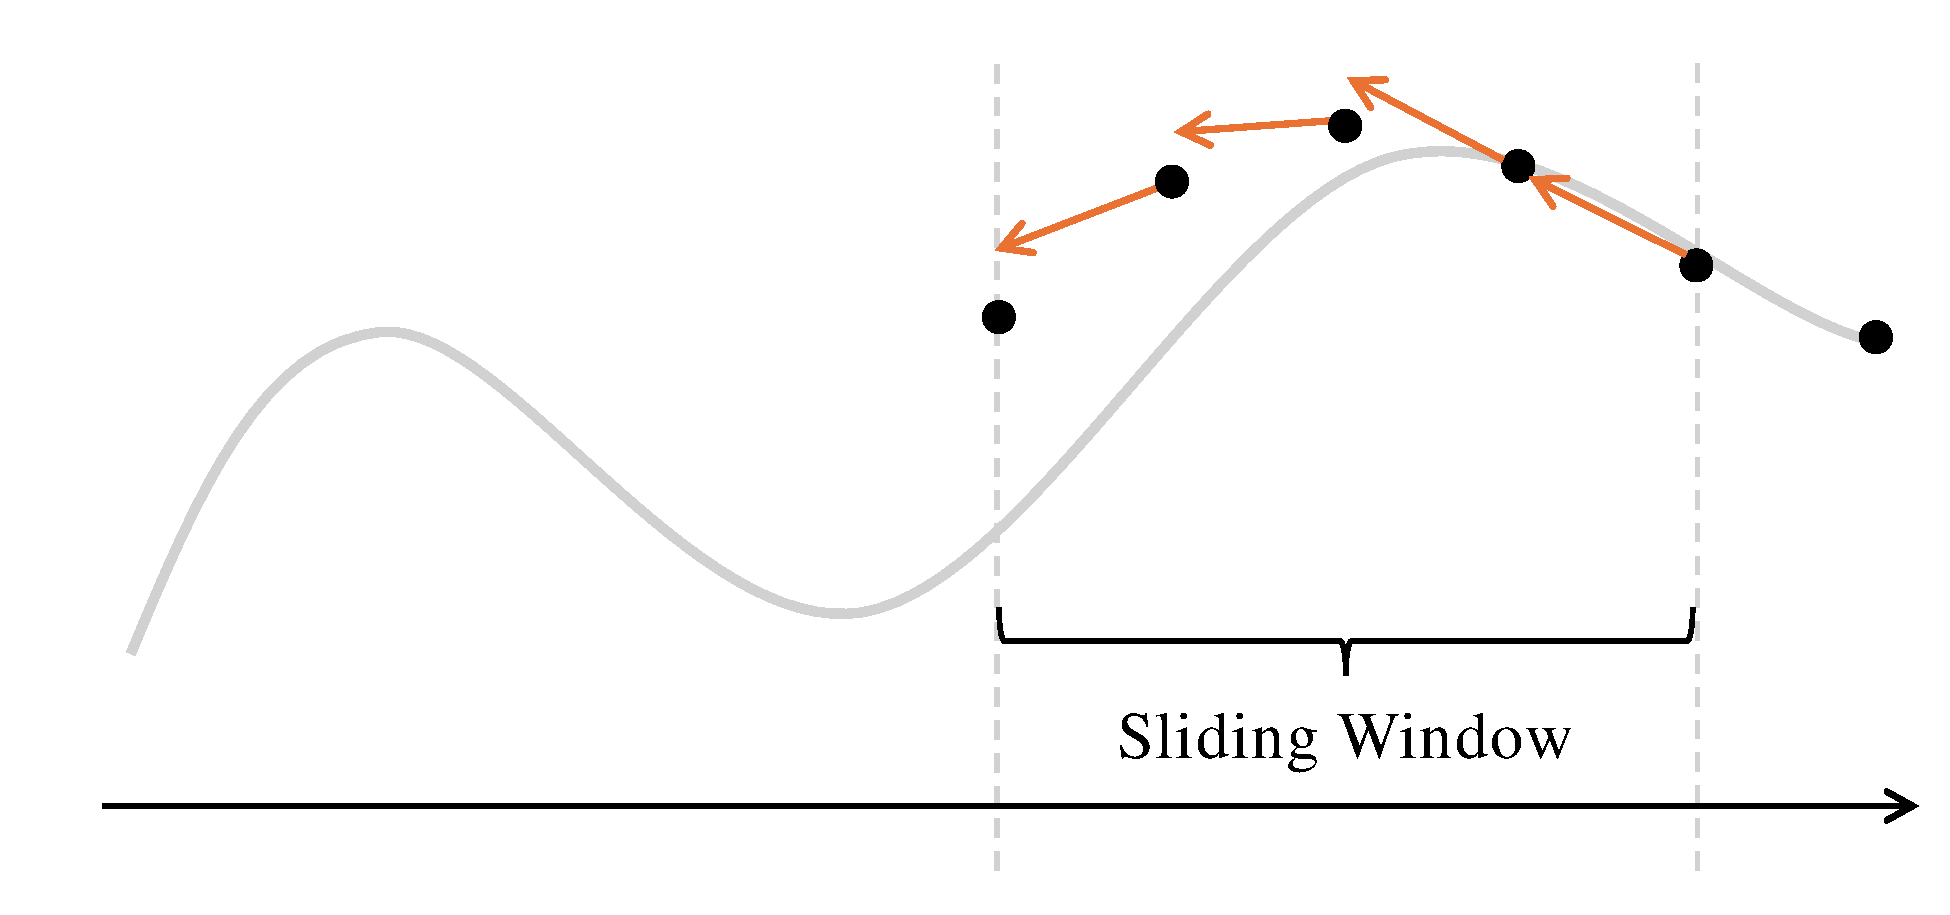
\includegraphics[width=\linewidth]{Images/PartC/paradigm-1.pdf}
        \caption{在大小为 $p=4$ 的批次窗口上并行计算 $\rvx^{(k)}_{\ell:\ell+p}$ 的漂移}
        \label{fig:picard_1}
    \end{minipage}%
    \hspace{0.03\textwidth} % To maintain the space between the images
    \begin{minipage}[t]{0.30\textwidth}
        \centering
        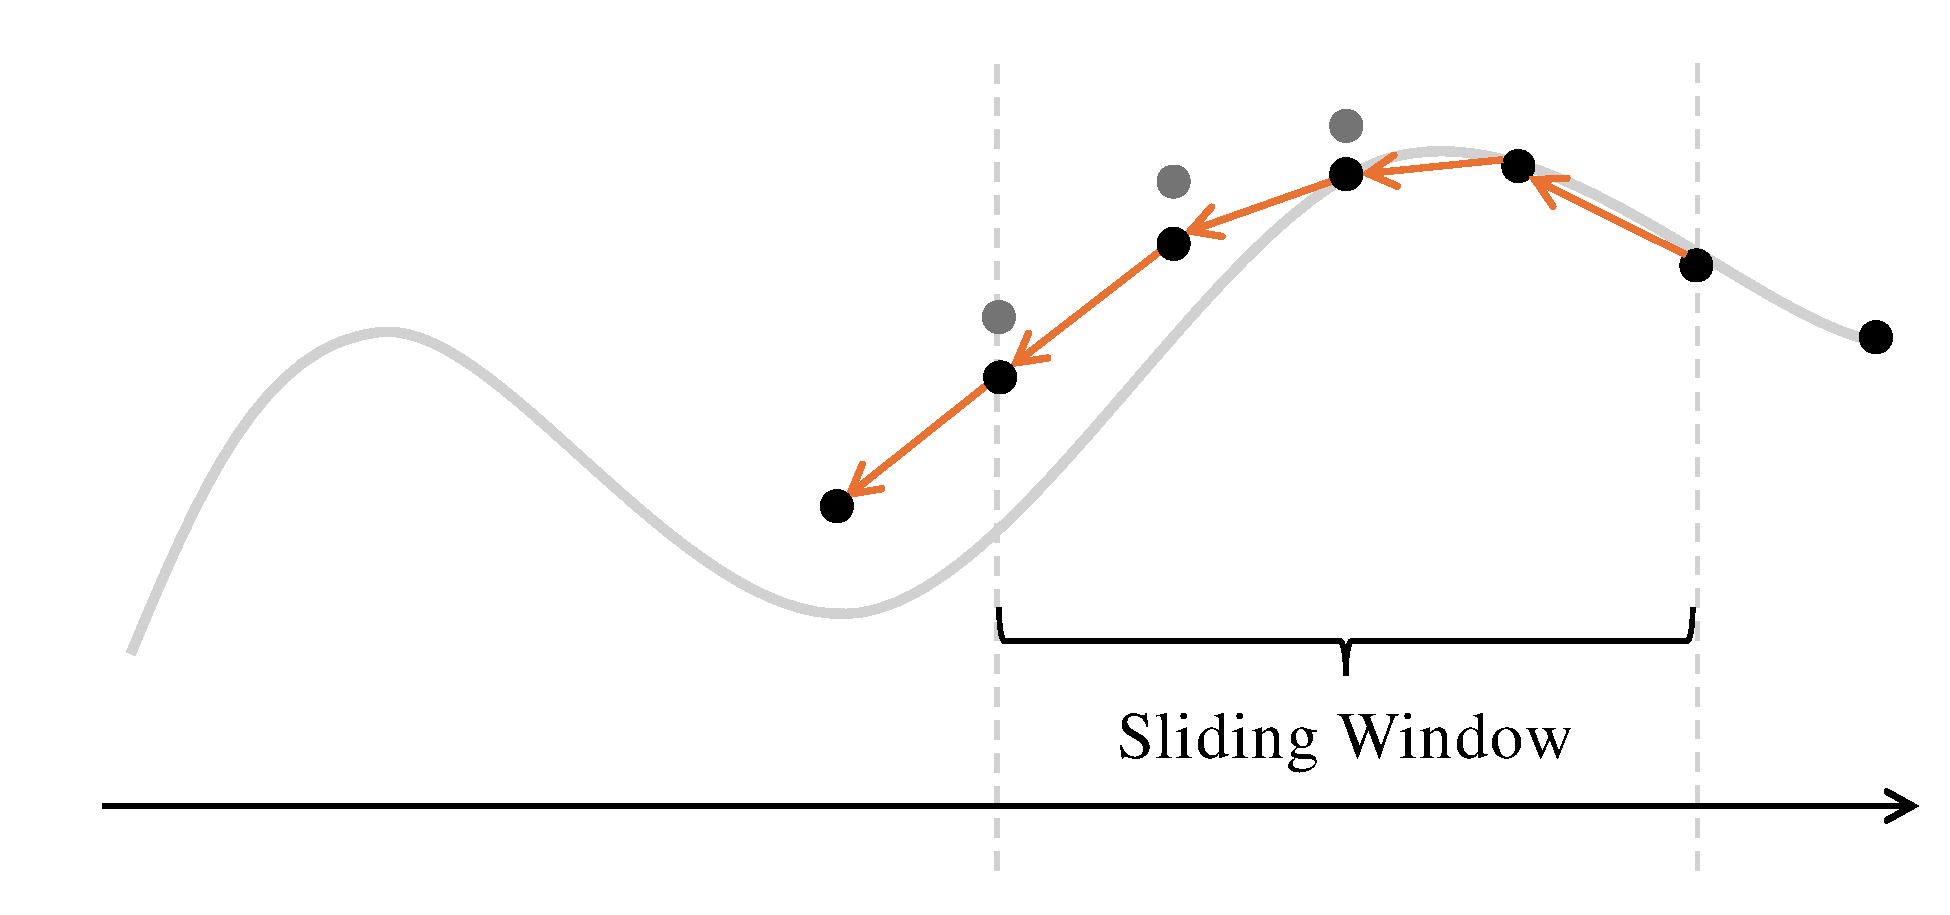
\includegraphics[width=\linewidth]{Images/PartC/paradigm-2.pdf}
        \caption{使用窗口内点的累积漂移更新值到 $\rvx^{(k+1)}_{\ell:\ell+p}$}
        \label{fig:picard_2}
    \end{minipage}%
    \hspace{0.03\textwidth} % To maintain the space between the images
    \begin{minipage}[t]{0.30\textwidth}
        \centering
        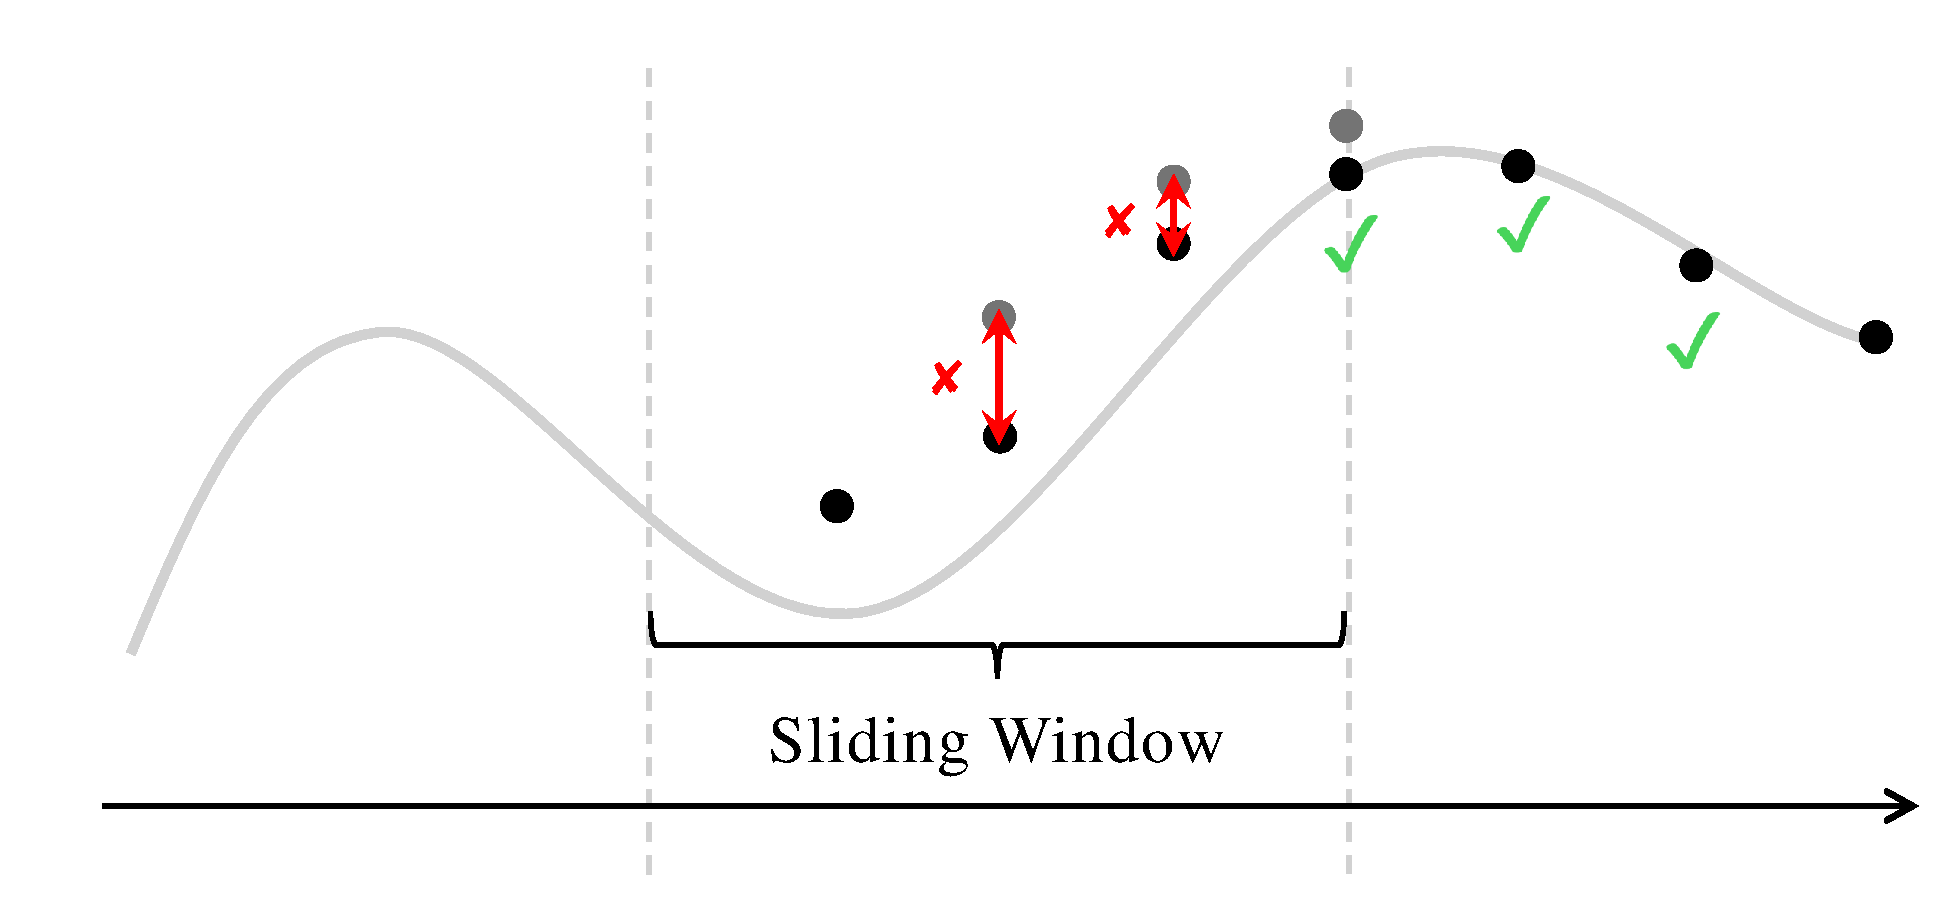
\includegraphics[width=\linewidth]{Images/PartC/paradigm-3.pdf}
        \caption{基于误差 $\lVert \rvx^{(k+1)}_i - \rvx^{(k)}_i \rVert^2$ 决定窗口向前滑动多远。}
        \label{fig:picard_3}
    \end{minipage}
    % \caption{During iteration $k$, ParaDiGMS processes a batch window of size $p$ spanning timesteps $[t,t+p)$ \textit{in parallel}. The new values at a point $\rvx^{(k+1)}_{t+j}$ are updated based on the value  $\rvx^{(k)}_j$ at the left end of the window, plus the cumulative drift  $1/T \sum_{i=t}^{t+j-1} \mathbf{F}_{\bm{\phi}^\times}(\rvx^{(k)}_{i}, i/T)$  of points within the window. We then slide the window forward until the error exceeds our tolerance, and repeat for the next iteration.}
    \figcredit{改编自 \citet{shih2023parallel}。}
    \label{fig:picard}
\end{figure}


离散 Picard 更新 \Cref{eq:discrete_picard_decreasing} 把每个 $\rvx^{(k+1)}_j$ 表示为左锚定的值 $\rvx^{(k)}_0$ 减去漂移的累加和。为限制内存并利用并行硬件，方便的做法是
把同一思想局部地应用于短的、滑动的索引块上。

固定窗口长度 $p$ 与左索引 $\ell$；则窗口覆盖
$j=\ell,\ldots,\ell+p$，其中 $t_\ell>t_{\ell+1}>\cdots>t_{\ell+p}$。在第
$k$ 次迭代中：

\subparagraph{第 1 步。窗口上的并行漂移求值。}
并行地、仅用上一次迭代，计算
\[
\rvv_{\bphi^\times} \big(\rvx^{(k)}_{\ell+i}, t_{\ell+i}\big),
\quad i=0,1,\ldots,p-1.
\]
它们是从左边缘
$t_\ell$ 跨越窗口推进所需的 $p$ 个局部增量。

\subparagraph{第 2 步。左锚定的累积更新。}
以 $j=\ell$ 锚定并跨子区间累积漂移，形成窗口化更新：
\begin{equation}\label{eq:window_update}
\rvx^{(k+1)}_{\ell+j+1}
 = 
\rvx^{(k)}_{\ell}
 - \Delta t \sum_{i=0}^{j}
\rvv_{\bphi^\times} \big(\rvx^{(k)}_{\ell+i}, t_{\ell+i}\big),
\quad j=0,1,\ldots,p-1.
\end{equation}
这正是 \Cref{eq:discrete_picard_decreasing} 限制在
窗口上的情形，减号反映了递减的时间方向。内层
求和是窗口化漂移上的前缀和（扫描），因此所有部分和
都可以在并行硬件上高效产生。

\subparagraph{第 3 步。进度控制与窗口推进。}
在当前窗口上形成左锚定的累积更新（第 2 步）之后，
我们现在决定该窗口向前滑动多远。我们用逐点 Picard 变化量
\[
\mathtt{error}_j
:=
\big\|\rvx^{(k+1)}_{\ell+j}-\rvx^{(k)}_{\ell+j}\big\|^2,
\quad j=1,\ldots,p-1,
\]
度量局部收敛性，
并将其与规定的容差 $\mathtt{tol}_{\ell+j}$ 比较。即 $\mathtt{error}_j$ 度量节点 $\ell+j$ 处的迭代在上一次 Picard
更新中变化了多少。若该值很小，则表明两次相继近似在该节点处的局部一致，从而该节点处的不动点
迭代局部收敛。若该值很大，则该节点尚未稳定，需要
更多 Picard 平滑。


\emph{步长}选为窗口中第一个未通过此检验的索引（若无失败则为完整窗口长度 $p$）：
\[
\mathtt{stride}
:=
\min\Big(\,\{\,j\ge 1:\ \mathtt{error}_j>\mathtt{tol}_{\ell+j}\,\}\ \cup\ \{p\}\Big).
\]
然后我们通过令 $\ell \leftarrow \ell+\mathtt{stride}$ 来滑动窗口。换言之：我们接受从左边缘起直至（但不包括）第一个未收敛节点的所有节点；若所有节点都已收敛，我们接受
整个窗口。然后我们按所接受的节点数滑动窗口，
$\ell \leftarrow \ell+\mathtt{stride}$，并继续。这最多前进
窗口长度 $p$，绝不跳过任何未达到其
容差的节点。若滑动会越过网格末端 $M$，我们把窗口截断为
$p \leftarrow \min\{p,\,M-\ell\}$ 并继续。



当窗口向前移动时，它会暴露出尚无
值的新时间节点。为在那里启动 Picard 迭代，我们简单地复制
窗口左边界处的值作为初始猜测。这种“常数外推”廉价且稳定，会被后续
更新修正。若需要，可用从过去点出发的线性
或多项式外推等更准确的猜测来替代它。

这就完成了 ParaDiGMS 的流程。我们在 \Cref{alg:paradigms} 中总结算法。


\begin{algorithm}[t]
  \caption{带滑动窗口的 ParaDiGMS}
  \label{alg:paradigms}
  \begin{algorithmic}[1]
    \Require 漂移 $\rvv_{\bphi^\times}(\rvx,t)$；$\{t_j\}_{j=0}^{M}$；窗口长度 $p$；$\{\mathtt{tol}_j\}_{j=1}^{M}$
    \Ensure 近似轨迹 $\{\rvx^{(k)}_j\}_{j=0}^{M}$，其中 $\rvx^{(k)}_M$ 在 $t=0$ 处
    \State $k \gets 0$, $\ell \gets 0$ 
    \State 采样 $\rvx^{(0)}_0 \sim p_{\mathrm{prior}}$；对 $j=1,\ldots,\min(p,M)$ 置 $\rvx^{(0)}_j \gets \rvx^{(0)}_0$  \Statex \Comment{常数外推}
    \While{$\ell < M$}
      \State $J \gets \min(p,  M-\ell)$   \Comment{当前窗口长度}
      \State \textbfs{第 1 步：并行} 
      \State 对 $i=0,\ldots,J-1$：$g_i \gets \rvv_{\bphi^\times} \big(\rvx^{(k)}_{\ell+i},\, t_{\ell+i}\big)$ 
      \Statex \Comment{来自上一次迭代的漂移（Picard 冻结）}
      \State 计算前缀和 $S_j \gets \sum_{i=0}^{j} g_i$，$j=0,\ldots,J-1$ 
      \Statex \Comment{对窗口化漂移做扫描}
      \State \textbfs{第 2 步：累积更新} 
      \State 对 $j=0,\ldots,J-1$：$\displaystyle \rvx^{(k+1)}_{\ell+j+1} \gets \rvx^{(k)}_{\ell} - \Delta t\, S_j$ 
      \Statex \Comment{左锚定更新；参见 \Cref{eq:window_update}}
      \State \textbfs{第 3 步：进度控制与窗口推进} 
      \State 对 $j=1,\ldots,J-1$：$\mathtt{error}_j \gets \big\|\rvx^{(k+1)}_{\ell+j}-\rvx^{(k)}_{\ell+j}\big\|^2$ \Statex \Comment{逐点 Picard 变化量}
      \State $\displaystyle \mathtt{stride} \gets \min \Big(\,\{\,j\in\{1,\ldots,J-1\}:~\mathtt{error}_j>\mathtt{tol}_{\ell+j}\,\}\ \cup\ \{J\}\Big)$
      \State \textbfs{初始化新节点} 
      \State 对 $r=1,\ldots,\mathtt{stride}$：$\rvx^{(k+1)}_{\ell+J+r} \gets \rvx^{(k+1)}_{\ell+J}$ 
      \Statex \Comment{对新暴露索引的常数外推}
      \State $\ell \gets \ell + \mathtt{stride}$;\quad $k \gets k+1$
    \EndWhile
    \State \Return $\{\rvx^{(k)}_j\}_{j=0}^{M}$
  \end{algorithmic}
\end{algorithm}




\subsection{与时间步进求解器的关系}

\paragraph{滑动窗口大小的选择。}

为把滑动窗口方案置于背景中，首先注意最小窗口大小时会发生什么。当 $p=1$ 时，窗口包含单步，故
\Cref{eq:window_update} 退化为 PF--ODE 的一阶时间步进更新。例如，若我们采用与 DDIM 相同的 ODE 写法（如数据 vs. 噪声预测）并选择与 DDIM 相同的离散时间步调度，则该方法退化为 DDIM。

增大 $p$ 扩展了并行性（每个窗口推进更多节点）而不
改变总步数 $M$。因此，样本质量继续
由基础离散化（网格/参数化的选择
和每步公式）连同每个窗口上的 Picard 收敛决定，
我们通过局部容差来监控。 

\paragraph{与高阶求解器（如 DPM）的兼容性。}
滑动窗口 Picard 结构控制的是增量\emph{如何}计算
（并行并由扫描累积），而不是\emph{哪个}局部公式定义
那些增量。因此，人们可以用任意
一致的高阶求积替换左端点规则而不改变并行
布局。例如，\Cref{eq:window_update} 的梯形变体为
\begin{align*}
    \begin{aligned}
        \rvx^{(k+1)}_{\ell+j+1}
=
\rvx^{(k)}_{\ell}
-\Delta t \Big[
\tfrac{1}{2}\rvv_{\bphi^\times} \big(\rvx^{(k)}_{\ell},t_{\ell}\big)
+\sum_{i=1}^{j-1}\rvv_{\bphi^\times} \big(\rvx^{(k)}_{\ell+i},t_{\ell+i}\big)
+\tfrac{1}{2}\rvv_{\bphi^\times} \big(\rvx^{(k)}_{\ell+j},t_{\ell+j}\big)
\Big],
    \end{aligned}
\end{align*}
其中所有漂移仍取自上一次 Picard 迭代，因此
逐节点求值保持独立，内层求和仍为前缀和。

类似地，DPM 求解器家族使用的多步或指数积分器更新
（例如 log--SNR 时间中的 DPM--Solver\texttt{++} $2$M）可以通过
用过去模型求值（$\rvx$-或 $\beps$-预测配以预计算
系数）的相应高阶线性组合替换每个窗口化增量来插入。
然后扫描像之前一样在窗口上累积那些加权增量。简言之：并行方案与近似积分的求解器（离散化）选择无关。精度来自基础求解器；窗口化前缀和只是让它变快。

\newpage
\section{结语}\label{sec:ch9_cr}

本章直面扩散模型最重要的实际局限之一：其缓慢的迭代采样过程。我们探索了一类强大的免训练解决方案，它们通过利用微分方程数值方法的丰富领域来加速生成。核心策略是更高效地求解 PF-ODE，该 ODE 定义了从噪声到数据的确定性生成轨迹：
\begin{enumerate}
    \item 我们从基础的 DDIM 开始，它可以被理解为一阶指数 Euler 方法。
    \item 然后转向像 DEIS 这样的高阶多步方法，它们通过使用过去求值的历史来提升精度。
    \item 最后，我们考察了高效的 DPM-Solver 家族，它通过引入关键的 log-SNR 时间重参数化实现了卓越的性能。
\end{enumerate}

通过这些高级求解器，高质量生成所需的函数评估次数（NFE）已从数百或数千次大幅减少到少至 10-20 次，使扩散模型显著更实用。

然而，这些免训练方法在根本仍然是迭代的。它们一步步地近似一条连续路径。这引出一个自然且雄心勃勃的问题：\emph{我们能否仅用一步或极少数离散步实现高质量生成？}

本书的最后部分 D 将通过基于训练的加速来探索这一问题。我们将研究两种主要策略：
\begin{enumerate}
    \item 首先，在 \Cref{ch:distillation} 中，我们将考察基于蒸馏的方法，其中一个快速的 \textit{学生} 生成器被训练以在远更少的步数内复现一个缓慢、预训练的 \textit{教师} 扩散模型的输出。
    \item 然后，在 \Cref{ch:fast-scratch} 中，我们将通过探索从头学习快速、少步生成器的方法把这一思想推得更远，例如一致性训练（Consistency Training），它定义了一种独立的训练原理而不依赖任何预训练模型。
\end{enumerate}

这种从改进求解器到直接学习解映射本身的转变，代表了高效生成式建模的前沿，旨在把扩散模型的质量与单步生成器的速度结合起来。


% \begin{itemize}
%     \item When $p=1$, ParaDiGMS reduces to the Euler method, equivalent to DDIM.
%     \item ParaDiGMS is compatible with any time-stepping ODE solver, including DDIM, DEIS, and the DPM-solvers family, among others.
%     \item ParaDiGMS does not degrade sample quality as it does not aim to reduce the number of sampling timesteps. 
% \end{itemize}


\clearpage
\newpage
